\documentclass[10pt,a4paper]{amsart}
\usepackage{amsmath,amssymb,amsthm,graphicx}
\usepackage{amsmath,amssymb,graphicx,xcolor,mathtools,listings}
\usepackage[no-math]{fontspec}
\newfontfamily\proofcodefont{DejaVu Sans}
\newfontfamily\proofwavefont{DejaVu Serif}
\lstset{basicstyle=\proofcodefont\tiny,breaklines=true,columns=fullflexible,keepspaces=true,escapeinside={(*@}{@*)}}
\title{Conditional soundness, termination and implementation completeness of a typed conversion checker}
\author{Meven Lennon-Bertrand}
\date{doi:10.4230/LIPIcs.FSCD.2025.27; CC BY4.0 (paper); MIT (author formal library)}
\begin{document}
\maketitle
\noindent\textit{Editorial note.} Paper https://drops.dagstuhl.de/entities/document/10.4230/LIPIcs.FSCD.2025.27, CC BY4.0. Complete author formal source archive is separately MIT, at snapshot9ca549d553bd41a6c00efb0655d23fa9a8dabd48 identified by the paper-linked Software Heritage revision.\par\medskip
\noindent\textit{Editorial note.} The counted result is the author package of conditional checker metatheorems, not a new certificate produced by collection. Each source proposition retains its own assumptions.\par\medskip
\noindent\textit{Allowed standard prerequisites (editorial).}\begin{itemize}
\item Dependent Martin-Löf type theory, de Bruijn substitution, and stated constructor-injectivity/deep-normalization properties. Author §2 and Properties1/11. These hypotheses are retained as the author states them. Full formal project, including all imported library support, is attached at the paper-linked snapshot.
\end{itemize}\medskip
% BEGIN S2
 
\par\medskip\noindent\textbf{2 The declarative system and its properties}\par
 
% BEGIN S2.SS1
 
\par\medskip\noindent\textbf{2.1 Definitions}\par
 
% BEGIN S2.SS1.SSS0.P0.SPx1
 
\par\medskip\noindent\textbf{The type system.}\par
 
% BEGIN S2.SS1.SSS0.P0.SPx1.p1
 
Our declarative type system and specification is a version of Martin-Löf’s type theory [40] with its five mutually defined judgments: typing of types, terms, and contexts and conversion (definitional equality) of types and terms, written $\mathrel{\raisebox{-0.5pt}{$\cong$}}$. They are defined as mutual inductive predicates on “raw” objects. We use $=$ to denote meta-level equality – which coincides $\alpha$-equality, as our representation uses pure de Bruijn indices.\par
 
% END S2.SS1.SSS0.P0.SPx1.p1
 
% BEGIN S2.SS1.SSS0.P0.SPx1.p2
 
The language supports dependent function ($\operatorname{\Pi}$) and pair ($\operatorname{\Sigma}$) types, which we call “negative”, with their $\beta$ and $\eta$-rules. We also include inductive types, with dependent large eliminators: an empty type $\operatorname{\bot}$, natural number type $\operatorname{\mathbb{N}}$, and an identity type $\operatorname{\mathbb{I}d}$. Finally, we have a universe $\operatorname{\mathcal{U}}$, with codes for all type formers except itself. We refer to these types as “positive”. Although our work does not directly involve focusing or logical polarity, where the positive/negative distinction stems from, it will still be an important distinction in the way our conversion algorithms work. We focus on $\operatorname{\mathcal{U}}$, $\operatorname{\Pi}$ and $\operatorname{\mathbb{N}}$ as representative examples on paper and direct interested readers to the code for others.\par
 
% END S2.SS1.SSS0.P0.SPx1.p2
 
% BEGIN S2.SS1.SSS0.P0.SPx1.p3
 
The development relies on parallel substitution, written $t\mathord{\left[\sigma\right]}$. If $u$ is a term, we also denote as $u$ the substitution mapping the last variable in context to $u$ and leaving all others untouched, as used in e.g. $\beta$-reduction: $(\operatorname{\lambda}x:A.t)\leavevmode\nobreak\ u\operatorname{\operatorname%
{\rightsquigarrow}^{\star}}t\mathord{\left[u\right]}$. In Rocq, we use AutoSubst 2 [46, 19] to generate boilerplate for the substitution calculus and automate tedious proofs with a decision procedure for meta-level equality of expressions in this calculus.\par
 
% END S2.SS1.SSS0.P0.SPx1.p3
 
% BEGIN S2.F2

\begin{center}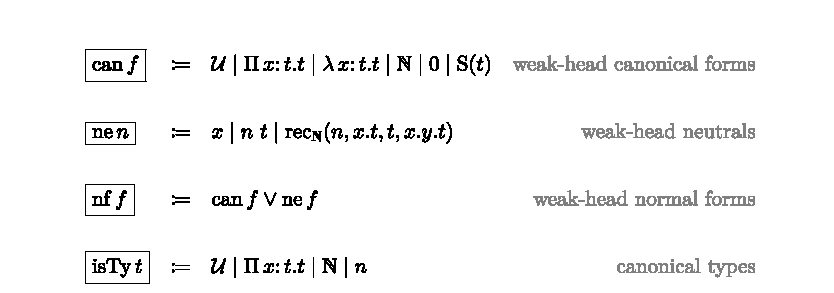
\includegraphics[width=0.98\linewidth,height=0.72\textheight,keepaspectratio]{rules-01.pdf}\end{center}
 
Figure 2:   Canonical, neutral, and normal form predicates (excerpt, see [34]). Way to read the BNF-style grammars: $\operatorname{isTy}$ is the predicate on terms given by the grammar $\operatorname{\mathcal{U}}\mid\operatorname{\Pi}x:t.t\mid\operatorname{\mathbb%
{N}}\mid n$ ($n$ stands for a neutral and $t$ for an arbitrary term).\par
 
% END S2.F2
 
% END S2.SS1.SSS0.P0.SPx1
 
% BEGIN S2.SS1.SSS0.P0.SPx2
 
\par\medskip\noindent\textbf{Normal forms and reduction.}\par
 
% BEGIN S2.SS1.SSS0.P0.SPx2.p1
 
Amongst terms, we particularly focus on (weak-head) normal forms, as this is the class with good injectivity properties, defined in Fig. 2. Canonical forms are terms starting with a constructor: $\operatorname{S}$, $\operatorname{\lambda}$, etc. Neutral forms are “stuck” terms, consisting of a spine of eliminators on top of a variable. Normal forms are either. We also define subclasses for each type: $\operatorname{isFun}t$ holds if $t$ is either a neutral or a $\operatorname{\lambda}$-abstraction, and similarly for $\operatorname{isTy}$ and $\operatorname{isNat}$. The $\operatorname{isTy_{+}}$ predicate isolates positive types: $\operatorname{\mathbb{N}}$, $\operatorname{\mathcal{U}}$ and neutrals.\par
 
% END S2.SS1.SSS0.P0.SPx2.p1
 
% BEGIN S2.F3

\begin{center}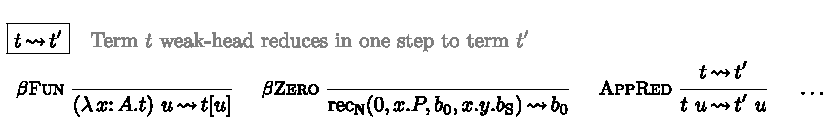
\includegraphics[width=0.98\linewidth,height=0.72\textheight,keepaspectratio]{rules-02.pdf}\end{center}
 
Figure 3:   Weak-head reduction (excerpt, see [34]).\par
 
% END S2.F3
 
% BEGIN S2.SS1.SSS0.P0.SPx2.p2
 
Finally, reduction $t\operatorname{\operatorname{\rightsquigarrow}^{\star}}t^{\prime}$ is the reflexive, transitive closure of one-step reduction, defined in Fig. 3. We use only a deterministic weak-head reduction. Reduction is not part of the specification of typing, we present it at this stage only to state normalisation in Sec. 2.2.\par
 
% END S2.SS1.SSS0.P0.SPx2.p2
 
% END S2.SS1.SSS0.P0.SPx2
 
% END S2.SS1
 
% BEGIN S2.SS2
 
\par\medskip\noindent\textbf{2.2 Meta-theory}\par
 
% BEGIN S2.SS2.p1
 
Let us now state the main meta-theoretic properties we consider – we comment about how to prove them at the end of this section and in Sec. 5. In Rocq, these are represented as type-classes: most theorems take instances of the relevant type-classes as parameters. This enables fine-grained bookkeeping of the theorems’ dependency, while keeping it lightweight as instances are automatically filled in. This is inspired by the treatment of function extensionality and univalence in the HoTT library [11].\par
 
% END S2.SS2.p1
 
% BEGIN S2.SS2.SSS0.P0.SPx1
 
\par\medskip\noindent\textbf{Type-level injectivity.}\par
 
% BEGIN Thmtheorem1
 
\par\medskip\noindent\textbf{Property 1 (  Injectivity and no-confusion of type constructors).}\par
 
% BEGIN Thmtheorem1.p1
 
Assume $T$ and $T^{\prime}$ are convertible types in weak-head normal form, i.e. we have that $\operatorname{isTy}T$, $\operatorname{isTy}T^{\prime}$, and $\Gamma\vdash T\mathrel{\raisebox{-0.5pt}{$\cong$}}T^{\prime}$. Then one of the following holds:\par
  
\par\noindent  $\blacksquare$ 
% BEGIN S2.I1.i1.p1
 
$T=\operatorname{\mathbb{N}}=T^{\prime}$ or $T=\operatorname{\mathcal{U}}=T^{\prime}$;\par
 
% END S2.I1.i1.p1
 
 
\par\noindent  $\blacksquare$ 
% BEGIN S2.I1.i2.p1
 
$T=\operatorname{\Pi}x:A.B$, $T^{\prime}=\operatorname{\Pi}x:A^{\prime}.B^{\prime}$, with $\Gamma\vdash A^{\prime}\mathrel{\raisebox{-0.5pt}{$\cong$}}A$ and $\Gamma,x:A^{\prime}\vdash B\mathrel{\raisebox{-0.5pt}{$\cong$}}B^{\prime}$;\par
 
% END S2.I1.i2.p1
 
 
\par\noindent  $\blacksquare$ 
% BEGIN S2.I1.i3.p1
 
$T$, $T^{\prime}$ are both neutral, and $\Gamma\vdash T\mathrel{\raisebox{-0.5pt}{$\cong$}}T^{\prime}\operatorname{%
\mathrel{:}}\operatorname{\mathcal{U}}$.\par
 
% END S2.I1.i3.p1
 
  
Any other case is thus impossible (no-confusion), e.g. we cannot have $\Gamma\vdash\operatorname{\Pi}x:A.B\mathrel{\raisebox{-0.5pt}{$\cong$}}%
\operatorname{\mathbb{N}}$.\par
 
% END Thmtheorem1.p1
 
% END Thmtheorem1
 
% BEGIN S2.SS2.SSS0.P0.SPx1.p1
 
This cannot be proven by mere induction, and indeed it implies a form of non-degeneracy, namely equational consistency: not all types are convertible. Consequences are numerous.\par
 
% END S2.SS2.SSS0.P0.SPx1.p1
 
% BEGIN Thmtheorem2
 
\par\medskip\noindent\textbf{Corollary 2 (  Preservation).}\par
 
% BEGIN Thmtheorem2.p1
 
Assuming Property 1, if $\Gamma\vdash A$ and $A\operatorname{\operatorname{\rightsquigarrow}^{\star}}A^{\prime}$ then $\Gamma\vdash A\mathrel{\raisebox{-0.5pt}{$\cong$}}A^{\prime}$. Similarly, if $\Gamma\vdash t\operatorname{\mathrel{:}}A$ and $t\operatorname{\operatorname{\rightsquigarrow}^{\star}}t^{\prime}$ then $\Gamma\vdash t\mathrel{\raisebox{-0.5pt}{$\cong$}}t^{\prime}\operatorname{%
\mathrel{:}}A$.\par
 
% END Thmtheorem2.p1
 
% END Thmtheorem2
 
% BEGIN Thmtheorem3
 
\par\medskip\noindent\textbf{Corollary 3 (  Types classify normal forms).}\par
 
% BEGIN Thmtheorem3.p1
 
Assuming Property 1, consider $t$ a normal form. If $\Gamma\vdash t\operatorname{\mathrel{:}}\operatorname{\Pi}x:A.B$, then $\operatorname{isFun}t$. If $\Gamma\vdash t\operatorname{\mathrel{:}}\operatorname{\mathbb{N}}$, then $\operatorname{isNat}t$. If $\Gamma\vdash t\operatorname{\mathrel{:}}\operatorname{\mathcal{U}}$, then $\operatorname{isTy}t$. If $\Gamma\vdash t\operatorname{\mathrel{:}}T$ and $T$ is neutral, then $t$ is neutral.\par
 
% END Thmtheorem3.p1
 
% END Thmtheorem3
 
% BEGIN S2.SS2.SSS0.P0.SPx1.p2
 
Preservation relies on the injectivity part, while classification uses no-confusion. Corollary 3 is the key lemma towards progress – the fact that every well-typed term is either a normal form or reduces –, although we do not show this in the formalisation. Thus, Property 1 suffices to establish safety in the progress-and-preservation approach [54].\par
 
% END S2.SS2.SSS0.P0.SPx1.p2
 
% END S2.SS2.SSS0.P0.SPx1
 
% BEGIN S2.SS2.SSS0.P0.SPx2
 
\par\medskip\noindent\textbf{Term-level injectivities.}\par
 
% BEGIN S2.SS2.SSS0.P0.SPx2.p1
 
Statements of injectivity (and no-confusion) for term constructors are relatively close to those for types.\par
 
% END S2.SS2.SSS0.P0.SPx2.p1
 
% BEGIN Thmtheorem4
 
\par\medskip\noindent\textbf{Property 4 (  Injectivity and no-confusion at $\operatorname{\mathbb{N}}$).}\par
 
% BEGIN Thmtheorem4.p1
 
Assume $n$ and $n^{\prime}$ are such that $\operatorname{isNat}n$, $\operatorname{isNat}n^{\prime}$, and $\Gamma\vdash n\mathrel{\raisebox{-0.5pt}{$\cong$}}n^{\prime}\operatorname{%
\mathrel{:}}\operatorname{\mathbb{N}}$. Then one of the following must hold:\par
  
\par\noindent  $\blacksquare$ 
% BEGIN S2.I2.i1.p1
 
$n=0=n^{\prime}$;\par
 
% END S2.I2.i1.p1
 
 
\par\noindent  $\blacksquare$ 
% BEGIN S2.I2.i2.p1
 
$n=\operatorname{S}(t)$, $n^{\prime}=\operatorname{S}(t^{\prime})$, with $\Gamma\vdash t\mathrel{\raisebox{-0.5pt}{$\cong$}}t^{\prime}\operatorname{%
\mathrel{:}}\operatorname{\mathbb{N}}$;\par
 
% END S2.I2.i2.p1
 
 
\par\noindent  $\blacksquare$ 
% BEGIN S2.I2.i3.p1
 
$n$, $n^{\prime}$ are both neutral.\par
 
% END S2.I2.i3.p1
 
  
% END Thmtheorem4.p1
 
% END Thmtheorem4
 
% BEGIN S2.SS2.SSS0.P0.SPx2.p2
 
Maybe surprisingly, the eliminator makes these statements directly provable. Indeed, assuming $\operatorname{S}(t)\mathrel{\raisebox{-0.5pt}{$\cong$}}\operatorname{S}(t^{%
\prime})$, by the computation and congruence rule for the eliminator, we get that $t\mathrel{\raisebox{-0.5pt}{$\cong$}}\operatorname{rec}_{\operatorname{\mathbb%
{N}}}(x.\operatorname{\mathbb{N}},\operatorname{S}(t),0,x.y.x)\mathrel{%
\raisebox{-0.5pt}{$\cong$}}\operatorname{rec}_{\operatorname{\mathbb{N}}}(x.%
\operatorname{\mathbb{N}},\operatorname{S}(t^{\prime}),0,x.y.x)\mathrel{%
\raisebox{-0.5pt}{$\cong$}}t^{\prime}\operatorname{\mathrel{:}}\operatorname{%
\mathbb{N}}$. We can similarly reduce no-confusion to that for types. A similar phenomenon happens at $\operatorname{\Pi}$ types, where injectivity of $\operatorname{\lambda}$ can also be directly derived.\par
 
% END S2.SS2.SSS0.P0.SPx2.p2
 
% BEGIN S2.SS2.SSS0.P0.SPx2.p3
 
Injectivity for the universe ( ) follows a similar pattern, but is not so easily proven for lack of an eliminator. For neutral types, which have no constructors, Corollary 3 is all we need: two (convertible) normal forms at a neutral type must be neutrals.\par
 
% END S2.SS2.SSS0.P0.SPx2.p3
 
% END S2.SS2.SSS0.P0.SPx2
 
% BEGIN S2.SS2.SSS0.P0.SPx3
 
\par\medskip\noindent\textbf{Neutral injectivities.}\par
 
% BEGIN S2.SS2.SSS0.P0.SPx3.p1
 
To complete the injectivity picture, we turn to neutrals, for which injectivity/no-confusion can be expressed in two ways. The first follows a familiar pattern.\par
 
% END S2.SS2.SSS0.P0.SPx3.p1
 
% BEGIN Thmtheorem5
 
\par\medskip\noindent\textbf{Property 5 (  Injectivity of neutral eliminators).}\par
 
% BEGIN Thmtheorem5.p1
 
Assume $n$ and $n^{\prime}$ are neutrals such that $\Gamma\vdash n\mathrel{\raisebox{-0.5pt}{$\cong$}}n^{\prime}\operatorname{%
\mathrel{:}}T$. Then one of the following must hold:\par
  
\par\noindent  $\blacksquare$ 
% BEGIN S2.I3.i1.p1
 
$n=x=n^{\prime}$, with $(x:T^{\prime})\in\Gamma$ and $\Gamma\vdash T^{\prime}\mathrel{\raisebox{-0.5pt}{$\cong$}}T$;\par
 
% END S2.I3.i1.p1
 
 
\par\noindent  $\blacksquare$ 
% BEGIN S2.I3.i2.p1
 
$n=m\ u$, $n^{\prime}=m^{\prime}\ u^{\prime}$ with $\Gamma\vdash m\mathrel{\raisebox{-0.5pt}{$\cong$}}m^{\prime}\operatorname{%
\mathrel{:}}\operatorname{\Pi}x:A.B$, $\Gamma\vdash u\mathrel{\raisebox{-0.5pt}{$\cong$}}u^{\prime}\operatorname{%
\mathrel{:}}A$ and $\Gamma\vdash B\mathord{\left[u\right]}\mathrel{\raisebox{-0.5pt}{$\cong$}}T$;\par
 
% END S2.I3.i2.p1
 
 
\par\noindent  $\blacksquare$ 
% BEGIN S2.I3.i3.p1
 
$n=\operatorname{rec}_{\operatorname{\mathbb{N}}}(m,x.P,t_{0},x.y.t_{%
\operatorname{S}})$, $n^{\prime}=\operatorname{rec}_{\operatorname{\mathbb{N}}}(m^{\prime},x.P^{%
\prime},t^{\prime}_{0},x.y.t^{\prime}_{\operatorname{S}})$, with convertible subterms.\par
 
% END S2.I3.i3.p1
 
  
% END Thmtheorem5.p1
 
% END Thmtheorem5
 
% BEGIN S2.SS2.SSS0.P0.SPx3.p2
 
However, in some cases this is too strong: at negative types our type-directed algorithm eagerly $\eta$-expands, so the above are only really needed at positive types. To state the “minimal” property we require, we take another way, starting with the following definition.\par
 
% END S2.SS2.SSS0.P0.SPx3.p2
 
% BEGIN Thmtheorem6
 
\par\medskip\noindent\textbf{Definition 6 (  Neutral comparison).}\par
 
% BEGIN Thmtheorem6.p1
 
Neutral comparison (see Sec. A.2), written $\Gamma\vdash n\sim n^{\prime}\operatorname{\mathrel{:}}T$, is the least relation that is:\par
  
\par\noindent  $\blacksquare$ 
% BEGIN S2.I4.i1.p1
 
reflexive on variables, i.e. $\Gamma\vdash x\sim x\operatorname{\mathrel{:}}T$ if $(x:T)\in\Gamma$;\par
 
% END S2.I4.i1.p1
 
 
\par\noindent  $\blacksquare$ 
% BEGIN S2.I4.i2.p1
 
closed under the congruence rules for eliminators;\par
 
% END S2.I4.i2.p1
 
 
\par\noindent  $\blacksquare$ 
% BEGIN S2.I4.i3.p1
 
stable under conversion: if $\Gamma\vdash n\sim n^{\prime}\operatorname{\mathrel{:}}T$ and $\Gamma\vdash T\mathrel{\raisebox{-0.5pt}{$\cong$}}T^{\prime}$ then $\Gamma\vdash n\sim n^{\prime}\operatorname{\mathrel{:}}T^{\prime}$.\par
 
% END S2.I4.i3.p1
 
  
% END Thmtheorem6.p1
 
% END Thmtheorem6
 
% BEGIN S2.SS2.SSS0.P0.SPx3.p3
 
We can then rephrase injectivity of neutral constructors as follows.\par
 
% END S2.SS2.SSS0.P0.SPx3.p3
 
% BEGIN Thmtheorem7
 
\par\medskip\noindent\textbf{Property 7 (  Completeness of neutral comparison).}\par
 
% BEGIN Thmtheorem7.p1
 
Given any two neutrals $n$ and $n^{\prime}$ such that $\Gamma\vdash n\mathrel{\raisebox{-0.5pt}{$\cong$}}n^{\prime}\operatorname{%
\mathrel{:}}T$, we have $\Gamma\vdash n\sim n^{\prime}\operatorname{\mathrel{:}}T$.\par
 
% END Thmtheorem7.p1
 
% END Thmtheorem7
 
% BEGIN Thmtheorem8
 
\par\medskip\noindent\textbf{Proposition 8 ( ).}\par
 
% BEGIN Thmtheorem8.p1
 
Property 5 and Property 7 are equivalent.\par
 
% END Thmtheorem8.p1
 
% END Thmtheorem8
 
% BEGIN S2.SS2.SSS0.P0.SPx3.p4
 
But now, we can weaken it to only consider positive types.\par
 
% END S2.SS2.SSS0.P0.SPx3.p4
 
% BEGIN Thmtheorem9
 
\par\medskip\noindent\textbf{Property 9 (  Completeness of neutral comparison at positive types).}\par
 
% BEGIN Thmtheorem9.p1
 
Given any two neutrals $n$ and $n^{\prime}$ such that $\Gamma\vdash n\mathrel{\raisebox{-0.5pt}{$\cong$}}n^{\prime}\operatorname{%
\mathrel{:}}T$, if moreover $\operatorname{isTy_{+}}T$, then we have $\Gamma\vdash n\sim n^{\prime}\operatorname{\mathrel{:}}T$.\par
 
% END Thmtheorem9.p1
 
% END Thmtheorem9
 
% END S2.SS2.SSS0.P0.SPx3
 
% BEGIN S2.SS2.SSS0.P0.SPx4
 
\par\medskip\noindent\textbf{Normalisation.}\par
 
% BEGIN S2.SS2.SSS0.P0.SPx4.p1
 
The last property is normalisation. Its main use is to argue for termination of the algorithm, so it has to go beyond weak-head reduction and take into account $\eta$-expansion, and subterms of (weak-head) normal forms.\par
 
% END S2.SS2.SSS0.P0.SPx4.p1
 
% BEGIN Thmtheorem10
 
\par\medskip\noindent\textbf{Definition 10 (  Deeply normalising).}\par
 
% BEGIN Thmtheorem10.p1
 
A term $t$ is deeply normalising at type $A$ in context $\Gamma$ if they reduce respectively to weak-head normal forms $t^{\prime}$ and $A^{\prime}$, and moreover:\par
  
\par\noindent  $\blacksquare$ 
% BEGIN S2.I5.i1.p1
 
$A^{\prime}$ is a negative type, and the $\eta$-expansion of $t^{\prime}$ is itself normalising;\par
 
% END S2.I5.i1.p1
 
 
\par\noindent  $\blacksquare$ 
% BEGIN S2.I5.i2.p1
 
or $A^{\prime}$ is a positive type, and the subterms of $t^{\prime}$ are normalising at the relevant types.\par
 
% END S2.I5.i2.p1
 
  
A type $A$ is deeply normalising in context $\Gamma$ if it reduces to a weak-head normal form, whose subterms are themselves normalising. See [34] for the inference rules.\par
 
% END Thmtheorem10.p1
 
% END Thmtheorem10
 
% BEGIN S2.SS2.SSS0.P0.SPx4.p2
 
While not apparent in this short version of the definition, the context actually plays a role in order to express the type at which a neutral should be normalising.\par
 
% END S2.SS2.SSS0.P0.SPx4.p2
 
% BEGIN Thmtheorem11
 
\par\medskip\noindent\textbf{Property 11 (  Deep normalisation).}\par
 
% BEGIN Thmtheorem11.p1
 
Every well-typed term is deeply normalising (at its type). Every well-formed type is deeply normalising.\par
 
% END Thmtheorem11.p1
 
% END Thmtheorem11
 
% BEGIN S2.SS2.SSS0.P0.SPx4.p3
 
Meta-theoretic consequences include canonicity ( ) – any closed term of type $\operatorname{\mathbb{N}}$ is convertible to one of the form $\operatorname{S}^{n}0$ – and, most importantly, logical consistency. This means that to prove Property 11, the meta-theory must be logically stronger than the object theory.\par
 
% END S2.SS2.SSS0.P0.SPx4.p3
 
% BEGIN Thmtheorem12
 
\par\medskip\noindent\textbf{Corollary 12 (  Logical consistency).}\par
 
% BEGIN Thmtheorem12.p1
 
Assuming Property 11, there are no closed terms of type $\operatorname{\bot}$.\par
 
% END Thmtheorem12.p1
 
% END Thmtheorem12
 
% END S2.SS2.SSS0.P0.SPx4
 
% BEGIN S2.SS2.SSS0.P0.SPx5
 
\par\medskip\noindent\textbf{Proving the properties.}\par
 
% BEGIN S2.SS2.SSS0.P0.SPx5.p1
 
In our formalisation, most properties are proven via a logical relation, in the style pioneered by Abel et al. [3], and later adapted in Rocq [7], to which we refer for details. Multiple universes in the meta-theory provide the logical strength we need to prove consistency. This approach is however by far not the only possibility, see the discussion in Sec. 5. Note the following two points.\par
 
% END S2.SS2.SSS0.P0.SPx5.p1
 
% BEGIN S2.SS2.SSS0.P0.SPx5.p2
 
First, the proof of deep normalisation is indirect. Indeed, the logical relation is parameterised by an abstract partial equivalence relation (PER) relating neutrals, which we instantiate with algorithmic neutral comparison to obtain normalisation for subterms of neutrals. To avoid this detour through algorithmic aspects, we envisioned strengthening the logical relation to directly encompass neutrals, but did not find a satisfying approach.\par
 
% END S2.SS2.SSS0.P0.SPx5.p2
 
% BEGIN S2.SS2.SSS0.P0.SPx5.p3
 
Second, as logical relations at negative types are naturally defined by observations (e.g. a function is reducible when its application to reducible inputs are reducible), these types “know nothing” about neutrals, and completeness of neutral comparison at negative types cannot be derived easily. We expect other proofs of “semantic” flavour to have similar issues with full completeness of neutrals, making the restriction to positive types (Property 9 vs. Property 7) an important distinction. And indeed, while completeness at positive types is a direct consequence of our logical relation ( ), the approach we found to completeness at all types takes a long detour via the two algorithmic presentations ( ) and strengthening.\par
 
% END S2.SS2.SSS0.P0.SPx5.p3
 
% END S2.SS2.SSS0.P0.SPx5
 
% END S2.SS2
 
% END S2


% BEGIN S3
 
\par\medskip\noindent\textbf{3 Algorithmic typing and conversion}\par
 
% BEGIN S3.p1
 
Let us now turn to our algorithms for conversion and typing. Only the untyped conversion algorithm is new, the typed conversion and bidirectional typing ones come directly from MLTT à la Coq [7]. We give the algorithms informally as rules, which are translated in the formalisation in two ways. First ( ) as inductively defined relations, like declarative typing. Second, we implement them as functions ( ). As we wish to separate their definition from their termination argument, we must embrace partiality. To that end, we use McBride’s free recursion monad [41], via Winterhalter’s PartialFun [53]. This lets us define the functions prior to any proofs; immediately execute them with bounded recursion depth – McBride’s “petrol semantics”; extract a typing (dis)proof from a terminating execution once we prove either soundness; and get proper decidability once we show normalisation. Cherry on the cake: as the recursion monad exposes the programs’ recursive structure, we can generically derive “functional” induction principles, following said recursive structures.\par
 
% END S3.p1
 
% BEGIN S3.SS0.SSS0.P0.SPx1
 
\par\medskip\noindent\textbf{Bidirectional typing.}\par
 
% BEGIN S3.SS0.SSS0.P0.SPx1.p1
 
Our typing algorithm, as most for dependent types, is bidirectional: it separates inference, written $\Gamma\vdash t\mathrel{\rhd}T$, where the type is an output to be found, from type checking, written $\Gamma\vdash t\operatorname{\mathrel{\lhd}}T$, where the type is a constraint given as input. We refer to others [42, 20, 31] for exposition – this last reference is the closest to us. Bidirectional typing generally has two main interests, although only the first is relevant to us here.\par
 
% END S3.SS0.SSS0.P0.SPx1.p1
 
% BEGIN S3.SS0.SSS0.P0.SPx1.p2
 
First, bidirectional typing gives better control over conversion. By replacing the conversion rule with syntax-directed rules, we get a term-directed system, amenable to implementation. This makes the bidirectional system a priori more restrictive than the declarative one, since we have strictly constrained the way conversion can be used. The main point of negative soundness is to show that this restriction does not, in fact, lose anything.\par
 
% END S3.SS0.SSS0.P0.SPx1.p2
 
% BEGIN S3.SS0.SSS0.P0.SPx1.p3
 
Second, propagating types “up” in derivations lightens the need for type annotations and gives better error messages. This is important for surface languages, less for kernels, where terms are typically not human-written. On the contrary, extra information can be useful in various ways, and we would rather dispense of the complication of segregating terms containing too little information to infer. Hence, as Rocq and Lean, we adopt a syntax where all terms infer, although completeness for the other approach is certainly interesting and feasible [35].\par
 
% END S3.SS0.SSS0.P0.SPx1.p3
 
% BEGIN S3.F4

\begin{center}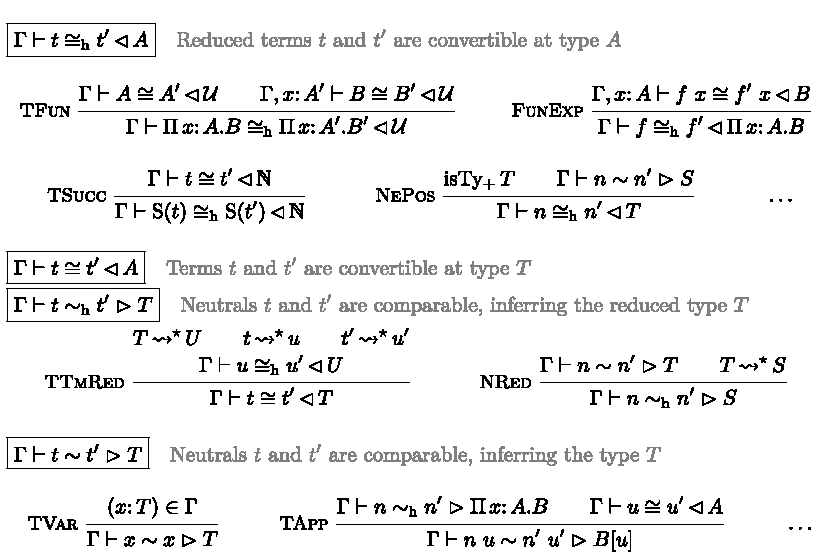
\includegraphics[width=0.98\linewidth,height=0.72\textheight,keepaspectratio]{rules-03.pdf}\end{center}
 
Figure 4:   Typed conversion algorithm (excerpt, see Sec. B.1).\par
 
% END S3.F4
 
% END S3.SS0.SSS0.P0.SPx1
 
% BEGIN S3.SS0.SSS0.P0.SPx2
 
\par\medskip\noindent\textbf{Typed conversion is bidirectional.}\par
 
% BEGIN S3.SS0.SSS0.P0.SPx2.p1
 
A point already implicitly present in Abel et al. [3], but made explicit in Adjedj et al. [7], is that the type-directed conversion algorithm is bidirectional, too. It is decomposed in two main functions, one to compare general terms and the other dedicated to neutrals. The former takes a type as input – it is checking –, while the latter reconstructs types as it traverses the neutrals – it is inferring.\par
 
% END S3.SS0.SSS0.P0.SPx2.p1
 
% BEGIN S3.SS0.SSS0.P0.SPx2.p2
 
More precisely, conversion (see Fig. 4), written $\Gamma\vdash t\mathrel{\raisebox{-0.5pt}{$\cong$}}u\operatorname{\mathrel{\lhd%
}}A$, goes as follows:\par
  
\par\noindent  1. 
% BEGIN S3.I1.i1.p1
 
reduce $t$, $u$ and $A$ to weak-head normal forms;\par
 
% END S3.I1.i1.p1
 
 
\par\noindent  2. 
% BEGIN S3.I1.i2.p1
 
if $A$ is a negative type ($\operatorname{\Pi},\operatorname{\Sigma}$), recursively compare the $\eta$-expansions of $t$ and $u$;\par
 
% END S3.I1.i2.p1
 
 
\par\noindent  3. 
% BEGIN S3.I1.i3.p1
 
if $A$ is a positive type ($\operatorname{\mathbb{N}},\operatorname{\mathcal{U}},\dots$) and the terms are canonical, use the relevant congruence;\par
 
% END S3.I1.i3.p1
 
 
\par\noindent  4. 
% BEGIN S3.I1.i4.p1
 
if $A$ is a positive type and the terms are neutrals, call neutral comparison.\par
 
% END S3.I1.i4.p1
 
  
Steps 2-4 are delegated to an auxiliary function, denoted $\mathrel{\raisebox{-0.5pt}{$\cong$}}_{\mathrm{h}}$ (the “h” is for “head”). Neutral comparison, written $\Gamma\vdash n\sim n^{\prime}\mathrel{\rhd}S$ follows their structure, applying congruences as it goes.\par
 
% END S3.SS0.SSS0.P0.SPx2.p2
 
% BEGIN S3.SS0.SSS0.P0.SPx2.p3
 
Rule   Typed conversion algorithm (excerpt, see Sec.˜B.1). demonstrates this bidirectional yoga. As conversion is type-directed, we need a type $A$ to compare the arguments, that is obtained through the recursive comparison of the functions, which must thus be inferring. We would not be able to construct $\operatorname{\Pi}x:A.B$ anyway, even given $B\mathord{\left[u\right]}$: inverting substitutions is unfeasible. Thus, even with a syntax with complete inference, the distinction between checking constructors and inferring eliminators, a landmark of the “Nordic” approach to bidirectionalism [43, 42], appears naturally.\par
 
% END S3.SS0.SSS0.P0.SPx2.p3
 
% END S3.SS0.SSS0.P0.SPx2
 
% BEGIN S3.SS0.SSS0.P0.SPx3
 
\par\medskip\noindent\textbf{Untyped conversion.}\par
 
% BEGIN S3.F5

\begin{center}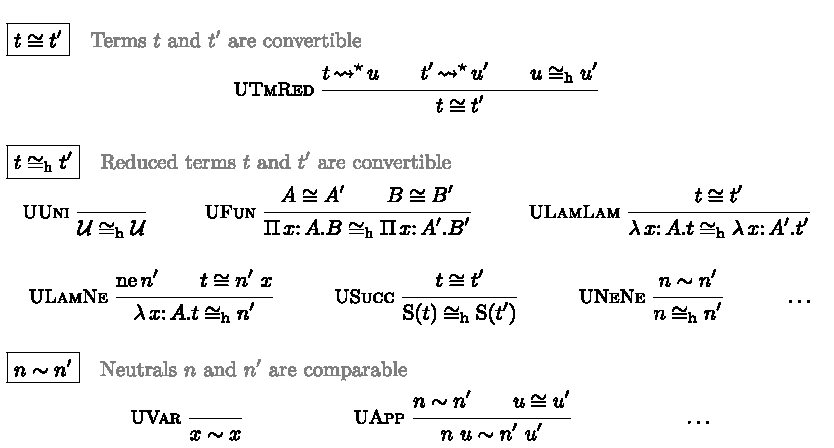
\includegraphics[width=0.98\linewidth,height=0.72\textheight,keepaspectratio]{rules-04.pdf}\end{center}
 
Figure 5:   Untyped algorithmic conversion (excerpt, see Sec. B.2).\par
 
% END S3.F5
 
% BEGIN S3.SS0.SSS0.P0.SPx3.p1
 
Untyped conversion (Fig. 5) looks much simpler than typed conversion: there are no types, no separation between type and term conversion, and the separation of neutral comparison is kept mostly for readability.\par
 
% END S3.SS0.SSS0.P0.SPx3.p1
 
% BEGIN S3.SS0.SSS0.P0.SPx3.p2
 
The main point is that we replace the all-encompassing   Typed conversion algorithm (excerpt, see Sec.˜B.1). by term-directed rules, an approach pioneered by Coquand, first for functions [16], then pairs [2]. When comparing $\operatorname{\lambda}$-abstractions, we apply the congruence   Untyped algorithmic conversion (excerpt, see Sec.˜B.2). – which would also happen in   Typed conversion algorithm (excerpt, see Sec.˜B.1). after contracting the redexes. If one side is a $\operatorname{\lambda}$ and the other a neutral (  Untyped algorithmic conversion (excerpt, see Sec.˜B.2).), we again simulate   Typed conversion algorithm (excerpt, see Sec.˜B.1)., but this time we see the application to a fresh variable is visible on the neutral’s side. And this is all! That is, there is no $\eta$-rule when the two sides are neutrals. How could there be? In the extreme case of two variables, the only information we could use is… type information, which we precisely decided not to rely on. This discrepancy on neutrals at negative types is the key difference between the two algorithms.\par
 
% END S3.SS0.SSS0.P0.SPx3.p2
 
% END S3.SS0.SSS0.P0.SPx3
 
% BEGIN S3.SS0.SSS0.P0.SPx4
 
\par\medskip\noindent\textbf{Comparison.}\par
 
% BEGIN S3.SS0.SSS0.P0.SPx4.p1
 
As a concrete example, we can look at the “execution trace” in the following problem: $x:\operatorname{\mathbb{N}}\to\operatorname{\mathbb{N}}\vdash x\mathrel{%
\raisebox{-0.5pt}{$\cong$}}x\operatorname{\mathrel{:}}\operatorname{\mathbb{N}%
}\to\operatorname{\mathbb{N}}$. The untyped algorithm immediately uses   Untyped algorithmic conversion (excerpt, see Sec.˜B.2). to go in “neutral mode”, and finishes with   Untyped algorithmic conversion (excerpt, see Sec.˜B.2).. The typed algorithm, on the other hand, first $\eta$-expands, introducing a fresh variable $y$, and recursively compares $x\ y$ to $x\ y$. Only then, by reaching a positive type, does it change to “neutral mode”. Neutral comparison then peels off the application node, compares $x$ to $x$ again but this time as neutrals, and finally applies variable reflexivity. It also needs to compare $y$ to $y$ first as normal forms at $\operatorname{\mathbb{N}}$, then as neutrals, and finally terminates. We can already see the work spared by the term-directed algorithm – exacerbated for $\operatorname{\Sigma}$ types, where $\eta$ introduces duplication.\par
 
% END S3.SS0.SSS0.P0.SPx4.p1
 
% END S3.SS0.SSS0.P0.SPx4
 
% END S3


% BEGIN S4.SS1
 
\par\medskip\noindent\textbf{4.1 Properties of typed conversion}\par
 
% BEGIN S4.SS1.p1
 
Most results in this section are not per se new, although they were significantly reworked, in particular to precisely track their dependencies. In particular, termination relies explicitly on normalisation, rather than on the reflexivity of the logical relation. The work around negative soundness is entirely new.\par
 
% END S4.SS1.p1
 
% BEGIN S4.SS1.SSS0.P0.SPx1
 
\par\medskip\noindent\textbf{Positive soundness.}\par
 
% BEGIN S4.SS1.SSS0.P0.SPx1.p1
 
We split the proof in two, using the inductive judgment as intermediate. The first half is almost tautological, and does not depend on any meta-theory.\par
 
% END S4.SS1.SSS0.P0.SPx1.p1

% BEGIN A1
 
\par\medskip\noindent\textbf{Appendix A Declarative Martin-Löf Type Theory}\par
 
% BEGIN A1.p1
 
On top of $t\mathord{\left[u\right]}$ for the substitution of the last variable of $t$ by $u$, we more generally use $t\mathord{\left[u,v,w\right]}$ for the parallel substitution of the last variables of $t$ with $u$, $v$ and $w$.\par
 
% END A1.p1
 
% BEGIN A1.SS1
 
\par\medskip\noindent\textbf{A.1 Declarative conversion}\par
 
% BEGIN A1.SS1.p1
 
\begin{center}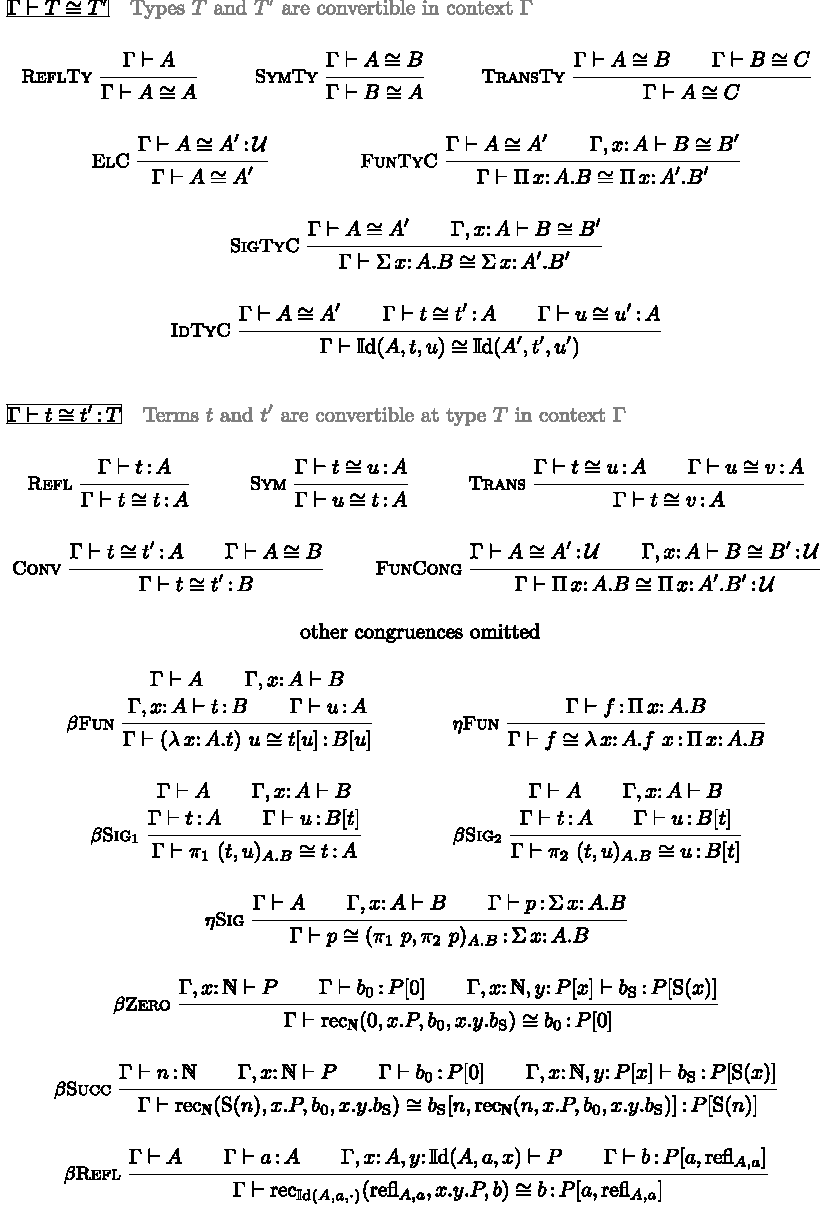
\includegraphics[width=0.98\linewidth,height=0.72\textheight,keepaspectratio]{rules-05.pdf}\end{center}
 
% END A1.SS1.p1
 
% END A1.SS1
 
% BEGIN A1.SS2
 
\par\medskip\noindent\textbf{A.2 Neutral comparison}\par
 
% BEGIN A1.SS2.p1
 
\begin{center}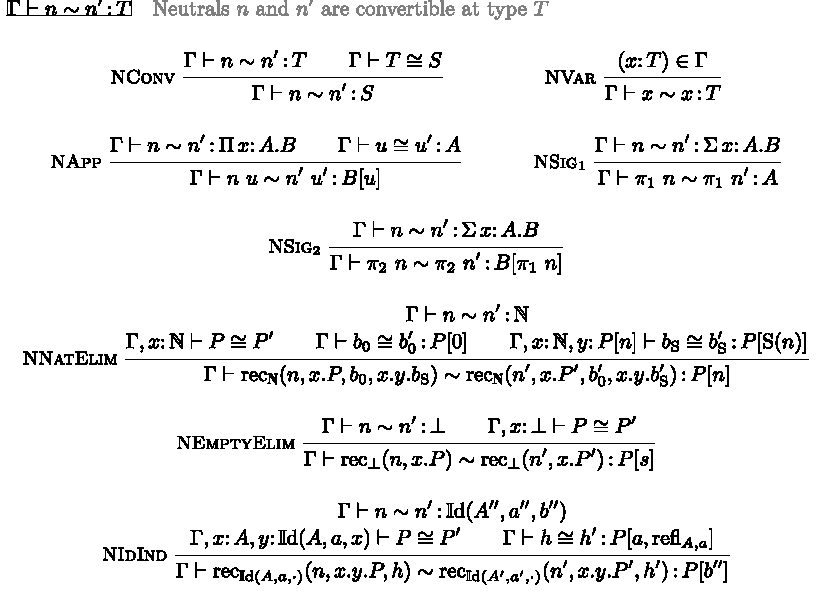
\includegraphics[width=0.98\linewidth,height=0.72\textheight,keepaspectratio]{rules-06.pdf}\end{center}
 
% END A1.SS2.p1
 
% END A1.SS2
 
% END A1


% BEGIN A2
 
\par\medskip\noindent\textbf{Appendix B Algorithmic Martin-Löf Type Theory}\par
 
% BEGIN A2.SS1
 
\par\medskip\noindent\textbf{B.1 Typed algorithmic conversion}\par
 
% BEGIN A2.SS1.p1
 
\begin{center}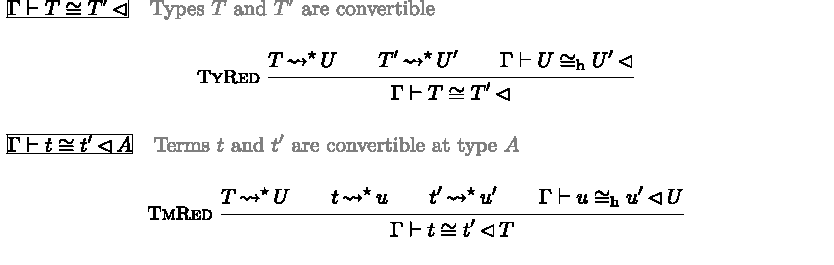
\includegraphics[width=0.98\linewidth,height=0.72\textheight,keepaspectratio]{rules-07.pdf}\end{center}
 
% END A2.SS1.p1
 
% BEGIN A2.SS1.p2
 
\begin{center}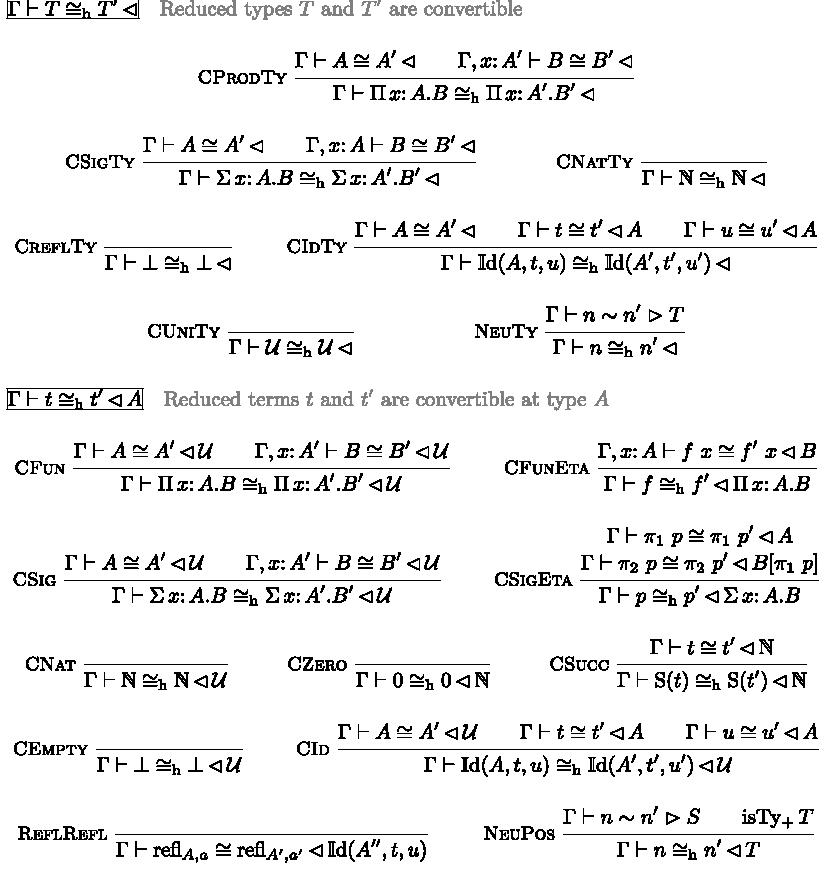
\includegraphics[width=0.98\linewidth,height=0.72\textheight,keepaspectratio]{rules-08.pdf}\end{center}
 
% END A2.SS1.p2
 
% BEGIN A2.SS1.p3
 
\begin{center}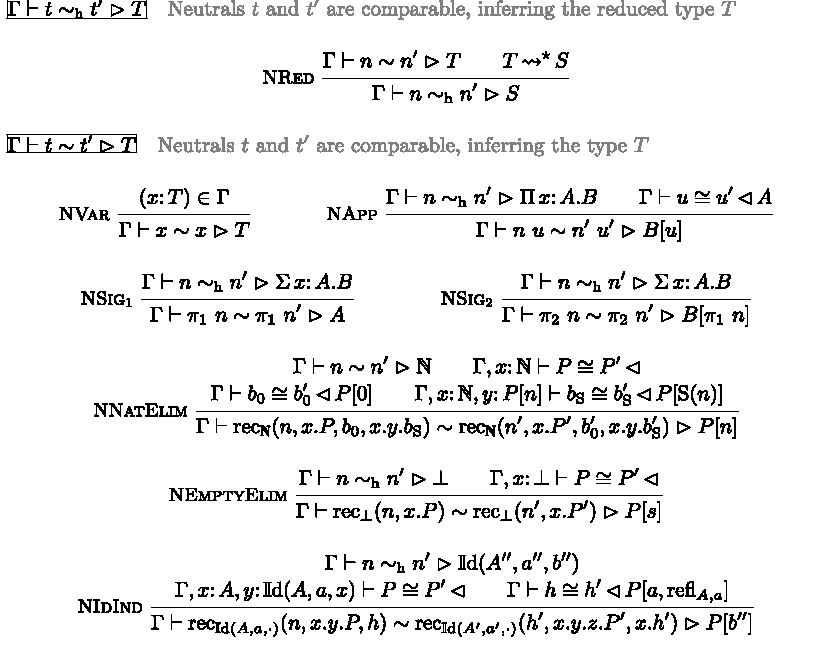
\includegraphics[width=0.98\linewidth,height=0.72\textheight,keepaspectratio]{rules-09.pdf}\end{center}
 
% END A2.SS1.p3
 
% END A2.SS1
 
% BEGIN A2.SS2
 
\par\medskip\noindent\textbf{B.2 Untyped algorithmic conversion}\par
 
% BEGIN A2.SS2.p1
 
\begin{center}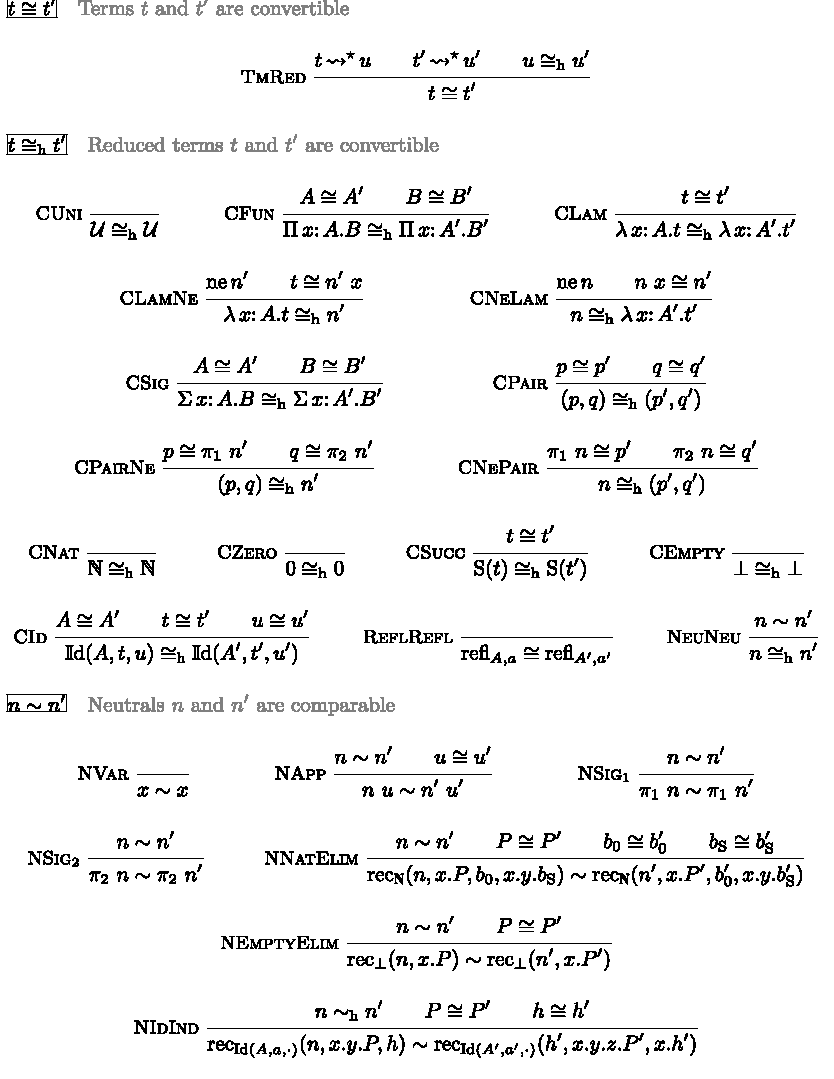
\includegraphics[width=0.98\linewidth,height=0.72\textheight,keepaspectratio]{rules-10.pdf}\end{center}
 
% END A2.SS2.p1
 
% BEGIN A2.SS2.p2
 
\par
 
% END A2.SS2.p2
 
% END A2.SS2
 
% END A2

% BEGIN Thmtheorem13
 
\par\medskip\noindent\textbf{Proposition 13 (  Positive soundness of the typed conversion function).}\par
 
% BEGIN Thmtheorem13.p1
 
If a typed conversion function returns a positive answer, then the corresponding judgment of Fig. 4 holds.\par
 
% END Thmtheorem13.p1
 
% END Thmtheorem13
 
% BEGIN Thmtheorem14
 
\par\medskip\noindent\textbf{Proposition 14 (  Positive soundness of the typed algorithmic conversion judgment).}\par
 
% BEGIN Thmtheorem14.p1
 
Assuming injectivity of type constructors (Property 1), the algorithmic typed conversion judgments imply their postconditions whenever their preconditions hold.\par
 
% END Thmtheorem14.p1
 
% END Thmtheorem14

% BEGIN Thmtheorem15
 
\par\medskip\noindent\textbf{Proposition 15 (  Negative soundness of typed algorithmic conversion).}\par
 
% BEGIN Thmtheorem15.p1
 
Assuming injectivity of type and term constructors (Properties 1, 4, etc.), and completeness of neutral conversion at positive types (Property 9), if a typed conversion function returns a negative answer and its precondition holds, then its postcondition cannot hold.\par
 
% END Thmtheorem15.p1
 
% END Thmtheorem15

% BEGIN Thmtheorem17
 
\par\medskip\noindent\textbf{Proposition 17 (  Termination of typed algorithmic conversion).}\par
 
% BEGIN Thmtheorem17.p1
 
Assuming injectivity of type constructors (Property 1) and deep normalisation (Property 11), typed conversion functions terminate whenever their preconditions are satisfied.\par
 
% END Thmtheorem17.p1
 
% END Thmtheorem17

% BEGIN Thmtheorem18
 
\par\medskip\noindent\textbf{Proposition 18 (  Completeness of the implementation).}\par
 
% BEGIN Thmtheorem18.p1
 
Assuming injectivity of type constructors (Property 1), if an algorithmic conversion judgment and its precondition hold, then the corresponding function answers positively.\par
 
% END Thmtheorem18.p1
 
% END Thmtheorem18

% BEGIN S4.SS1.SSS0.P0.SPx1.p2
 
This second half is the interesting one. The crucial part of this proof, and the backbone of others in this section, is to show that each inductive rule correctly preserves the invariants. This is a very regular property, so much that we meta-programmed444 We hardcoded these in the current code to remove a dependency which caused proof engineering issues.  the generation of “local preservation lemmas” ( ) for each rule, expressing this idea. We assemble these lemmas into a “bundled induction principle”, again programmatically generated, which threads the invariants through, giving access to them as extra hypotheses in each induction step. Soundness follows by instantiating this induction principle with the constant True predicates.\par
 
% END S4.SS1.SSS0.P0.SPx1.p2
 
% END S4.SS1.SSS0.P0.SPx1
 
% BEGIN S4.SS1.SSS0.P0.SPx2
 
\par\medskip\noindent\textbf{Negative soundness.}\par
 
% BEGIN S4.SS1.SSS0.P0.SPx2.p1
 
For negative soundness, we cannot go through the intermediate algorithmic judgments, as they only encode successful runs of the functions. Thus, we bite the bullet and directly relate the output of the functions to the declarative judgments.\par
 
% END S4.SS1.SSS0.P0.SPx2.p1

% BEGIN S4.SS1.SSS0.P0.SPx2.p2
 
Again, we rely on invariant preservation, the proof is otherwise straightforward: we have extracted exactly the injectivity properties needed to justify each step. In essence, we show that at any stage the current “remaining goals” are equivalent to the initial query, relying on injectivity to know that we only use invertible congruences, which are safe to apply.\par
 
% END S4.SS1.SSS0.P0.SPx2.p2
 
% END S4.SS1.SSS0.P0.SPx2
 
% BEGIN S4.SS1.SSS0.P0.SPx3
 
\par\medskip\noindent\textbf{Termination.}\par
 
% BEGIN S4.SS1.SSS0.P0.SPx3.p1
 
As expected, this is where normalisation becomes necessary. As before, we need invariants throughout, and thus injectivity of type constructors. The most subtle part of the proof concerns the reduction machine.\par
 
% END S4.SS1.SSS0.P0.SPx3.p1
 
% BEGIN Thmtheorem16
 
\par\medskip\noindent\textbf{Lemma 16 (  Completeness of reduction).}\par
 
% BEGIN Thmtheorem16.p1
 
Assuming Property 1, if $t$ is well-typed and reduces to the weak-head normal form $t^{\prime}$, then the reduction function applied to $t$ returns $t^{\prime}$.\par
 
% END Thmtheorem16.p1
 
% END Thmtheorem16
 
% BEGIN S4.SS1.SSS0.P0.SPx3.p2
 
The main task is to define a well-founded order on the configurations of the abstract machine implementing reduction, a lexicographic product of subterm ordering and reduction. The assumption that $t$ reduces to a weak-head normal form ensures that this order is well-founded. Winterhalter introduced a similar order for MetaCoq [52, chap. 23].\par
 
% END S4.SS1.SSS0.P0.SPx3.p2

% BEGIN S4.SS1.SSS0.P0.SPx3.p3
 
The proof is by induction on deep normalisation, again using local preservation lemmas. The inductive structure of deep normalisation readily encodes the combination of subterm, reduction and $\eta$-expansion that one needs to be well-founded. In contrast, in MetaCoq, Winterhalter introduced a complex dependent lexicographic order modulo [52, chap 24], and admits that his setup would not easily incorporate $\eta$-expansion.\par
 
% END S4.SS1.SSS0.P0.SPx3.p3
 
% END S4.SS1.SSS0.P0.SPx3
 
% BEGIN S4.SS1.SSS0.P0.SPx4
 
\par\medskip\noindent\textbf{Non-triviality.}\par
 
% BEGIN S4.SS1.SSS0.P0.SPx4.p1
 
Soundness, both positive and negative, has a default: the nowhere-defined function is sound! Although we repeat that these properties should not be read to merely say “there exists a function such that…” but to characterise a particular checker – that we can run on examples ( ) to check for non-triviality –, it is good to formally ensure that our functions are non-trivial. Again, this is split in two.\par
 
% END S4.SS1.SSS0.P0.SPx4.p1

% BEGIN S4.SS1.SSS0.P0.SPx4.p2
 
Next, we show that algorithmic conversion satisfies many closure properties, which Abel et al. call “generic conversion”. These are rather rich: all the proofs on the logical relation side can be done with respect to any generic conversion.\par
 
% END S4.SS1.SSS0.P0.SPx4.p2
 
% BEGIN Thmtheorem19
 
\par\medskip\noindent\textbf{Proposition 19 ( ).}\par
 
% BEGIN Thmtheorem19.p1
 
Algorithmic conversion is a generic conversion, thus for instance symmetric and transitive, stable by weakening and expansion, congruent for constructors.\par
 
% END Thmtheorem19.p1
 
% END Thmtheorem19
 
% BEGIN S4.SS1.SSS0.P0.SPx4.p3
 
Compared to declarative typing, the only missing part is congruences for eliminators, which only hold for neutral conversion, and reflexivity – which would be direct by induction if we had all congruence rules. The point is that eliminator congruences are the dangerous ones that can trigger reductions: applying a normal form to a normal form does not yield a normal form. And indeed a term is deeply normalising exactly when it is reflexive for (typed) algorithmic conversion, explaining why reflexivity cannot be achieved easily.\par
 
% END S4.SS1.SSS0.P0.SPx4.p3
 
% END S4.SS1.SSS0.P0.SPx4
 
% BEGIN S4.SS1.SSS0.P0.SPx5
 
\par\medskip\noindent\textbf{Typing.}\par
 
% BEGIN S4.SS1.SSS0.P0.SPx5.p1
 
All of these propositions extend to bidirectional typing. More precisely, assuming any conversion relation/function between types that satisfies the relevant property, we can derive a similar one for typing. This means that the proofs are modular, in that we can swap out a different implementation of conversion, as long as it satisfies the right properties, which is exactly what we are about to do.\par
 
% END S4.SS1.SSS0.P0.SPx5.p1
 
% END S4.SS1.SSS0.P0.SPx5
 
% END S4.SS1

\clearpage
\section*{Author typed-checker implementation and complete correctness proof modules}
Complete original modules below come from the paper-linked MIT source snapshot 9ca549d553bd41a6c00efb0655d23fa9a8dabd48. The complete source project with all imports is also attached. No checker execution or certification is performed by collection.

\subsection*{theories/DeclarativeTyping.v}
\begin{lstlisting}
(** * LogRel.DeclarativeTyping: specification of conversion and typing, in a declarative fashion. *)
From Coq Require Import ssreflect.
From smpl Require Import Smpl.
From LogRel Require Import Utils Syntax.All.

Set Primitive Projections.

(** Definitions in this file should be understood as the _specification_ of conversion
or typing, done in a declarative fashion. For instance, we _demand_ that conversion
be transitive by adding a corresponding rule. *)

(** ** Definitions *)
Section Definitions.

  (* We locally disable typing notations to be able to use them in the definition
  here before declaring the instance to which abstract notations are bound. *)
  Close Scope typing_scope.


  (** Typing and conversion are mutually defined inductive relations. To avoid having
  to bother with elimination of propositions, we put them in the Type sort. *)

  (** **** Context well-formation *)
  Inductive WfContextDecl : context -> Type :=
      | connil : [ |- ε ]
      | concons {Γ A} : 
          [ |- Γ ] -> 
          [ Γ |- A ] -> 
          [ |-  Γ ,, A]
  (** **** Type well-formation *)
  with WfTypeDecl  : context -> term -> Type :=
      | wfTypeU {Γ} : 
          [ |- Γ ] -> 
          [ Γ |- U ] 
      | wfTypeProd {Γ} {A B} : 
          [ Γ |- A ] -> 
          [Γ ,, A |- B ] -> 
          [ Γ |- tProd A B ]
      | wfTypeNat {Γ} : 
          [|- Γ] ->
          [Γ |- tNat]
      | wfTypeEmpty {Γ} : 
          [|- Γ] ->
          [Γ |- tEmpty]
      | wfTypeSig {Γ} {A B} : 
          [ Γ |- A ] -> 
          [Γ ,, A |- B ] -> 
          [ Γ |- tSig A B ]
      | wftTypeId {Γ} {A x y} :
          [Γ |- A] ->
          [Γ |- x : A] ->
          [Γ |- y : A] ->
          [Γ |- tId A x y]
      | wfTypeUniv {Γ} {A} :
          [ Γ |- A : U ] -> 
          [ Γ |- A ]
  (** **** Typing *)
  with TypingDecl : context -> term -> term -> Type :=
      | wfVar {Γ} {n decl} :
          [   |- Γ ] ->
          in_ctx Γ n decl ->
          [ Γ |- tRel n : decl ]
      | wfTermProd {Γ} {A B} :
          [ Γ |- A : U] -> 
          [Γ ,, A |- B : U ] ->
          [ Γ |- tProd A B : U ]
      | wfTermLam {Γ} {A B t} :
          [ Γ |- A ] ->        
          [ Γ ,, A |- t : B ] -> 
          [ Γ |- tLambda A t : tProd A B]
      | wfTermApp {Γ} {f a A B} :
          [ Γ |- f : tProd A B ] -> 
          [ Γ |- a : A ] -> 
          [ Γ |- tApp f a : B[a..] ]
      | wfTermNat {Γ} :
          [|-Γ] ->
          [Γ |- tNat : U]
      | wfTermZero {Γ} :
          [|-Γ] ->
          [Γ |- tZero : tNat]
      | wfTermSucc {Γ n} :
          [Γ |- n : tNat] ->
          [Γ |- tSucc n : tNat]
      | wfTermNatElim {Γ P hz hs n} :
        [Γ ,, tNat |- P ] ->
        [Γ |- hz : P[tZero..]] ->
        [Γ |- hs : elimSuccHypTy P] ->
        [Γ |- n : tNat] ->
        [Γ |- tNatElim P hz hs n : P[n..]]
      | wfTermEmpty {Γ} :
          [|-Γ] ->
          [Γ |- tEmpty : U]
      | wfTermEmptyElim {Γ P e} :
        [Γ ,, tEmpty |- P ] ->
        [Γ |- e : tEmpty] ->
        [Γ |- tEmptyElim P e : P[e..]]
      | wfTermSig {Γ} {A B} :
        [ Γ |- A : U] -> 
        [Γ ,, A |- B : U ] ->
        [ Γ |- tSig A B : U ]
      | wfTermPair {Γ} {A B a b} :
        [Γ |- A] ->
        [Γ,, A |- B] ->
        [Γ |- a : A] -> 
        [Γ |- b : B[a..]] ->
        [Γ |- tPair A B a b : tSig A B]
      | wfTermFst {Γ A B p} :
        [Γ |- p : tSig A B] ->
        [Γ |- tFst p : A]
      | wfTermSnd {Γ A B p} :
        [Γ |- p : tSig A B] ->
        [Γ |- tSnd p : B[(tFst p)..]]
      | wfTermId {Γ} {A x y} :
          [Γ |- A : U] ->
          [Γ |- x : A] ->
          [Γ |- y : A] ->
          [Γ |- tId A x y : U]
      | wfTermRefl {Γ A x} :
          [Γ |- A] ->
          [Γ |- x : A] ->
          [Γ |- tRefl A x : tId A x x]
      | wfTermIdElim {Γ A x P hr y e} :
          [Γ |- A] ->
          [Γ |- x : A] ->
          [Γ ,, A ,, tId A⟨@wk1 Γ A⟩ x⟨@wk1 Γ A⟩ (tRel 0) |- P] ->
          [Γ |- hr : P[tRefl A x .: x..]] ->
          [Γ |- y : A] ->
          [Γ |- e : tId A x y] ->
          [Γ |- tIdElim A x P hr y e : P[e .: y..]]
      | wfTermConv {Γ} {t A B} :
          [ Γ |- t : A ] -> 
          [ Γ |- A ≅ B ] -> 
          [ Γ |- t : B ]
  (** **** Conversion of types *)
  with ConvTypeDecl : context -> term -> term  -> Type :=  
      | TypePiCong {Γ} {A B C D} :
          [ Γ |- A] ->
          [ Γ |- A ≅ B] ->
          [ Γ ,, A |- C ≅ D] ->
          [ Γ |- tProd A C ≅ tProd B D]
      | TypeSigCong {Γ} {A B C D} :
          [ Γ |- A] ->
          [ Γ |- A ≅ B] ->
          [ Γ ,, A |- C ≅ D] ->
          [ Γ |- tSig A C ≅ tSig B D]
      | TypeIdCong {Γ A A' x x' y y'} :
          (* [Γ |- A] -> ?  *)
          [Γ |- A ≅ A'] ->
          [Γ |- x ≅ x' : A] ->
          [Γ |- y ≅ y' : A] ->
          [Γ |- tId A x y ≅ tId A' x' y' ]
      | TypeRefl {Γ} {A} : 
          [ Γ |- A ] ->
          [ Γ |- A ≅ A]
      | convUniv {Γ} {A B} :
        [ Γ |- A ≅ B : U ] -> 
        [ Γ |- A ≅ B ]
      | TypeSym {Γ} {A B} :
          [ Γ |- A ≅ B ] ->
          [ Γ |- B ≅ A ]
      | TypeTrans {Γ} {A B C} :
          [ Γ |- A ≅ B] ->
          [ Γ |- B ≅ C] ->
          [ Γ |- A ≅ C]
  (** **** Conversion of terms *)
  with ConvTermDecl : context -> term -> term -> term -> Type :=
      | TermBRed {Γ} {a t A B} :
              [ Γ |- A ] ->
              [ Γ ,, A |- t : B ] ->
              [ Γ |- a : A ] ->
              [ Γ |- tApp (tLambda A t) a ≅ t[a..] : B[a..] ]
      | TermPiCong {Γ} {A B C D} :
          [ Γ |- A : U] ->
          [ Γ |- A ≅ B : U ] ->
          [ Γ ,, A |- C ≅ D : U ] ->
          [ Γ |- tProd A C ≅ tProd B D : U ]
      | TermAppCong {Γ} {a b f g A B} :
          [ Γ |- f ≅ g : tProd A B ] ->
          [ Γ |- a ≅ b : A ] ->
          [ Γ |- tApp f a ≅ tApp g b : B[a..] ]
      | TermLambdaCong {Γ} {t u A A' A'' B} :
          [ Γ |- A ] ->
          [ Γ |- A ≅ A' ] ->
          [ Γ |- A ≅ A'' ] ->
          [ Γ,, A |- t ≅ u : B ] ->
          [ Γ |- tLambda A' t ≅ tLambda A'' u : tProd A B ]
      | TermFunEta {Γ} {f A B} :
          [ Γ |- f : tProd A B ] ->
          [ Γ |- tLambda A (eta_expand f) ≅ f : tProd A B ]
      | TermSuccCong {Γ} {n n'} :
          [Γ |- n ≅ n' : tNat] ->
          [Γ |- tSucc n ≅ tSucc n' : tNat]
      | TermNatElimCong {Γ P P' hz hz' hs hs' n n'} :
          [Γ ,, tNat |- P ≅ P'] ->
          [Γ |- hz ≅ hz' : P[tZero..]] ->
          [Γ |- hs ≅ hs' : elimSuccHypTy P] ->
          [Γ |- n ≅ n' : tNat] ->
          [Γ |- tNatElim P hz hs n ≅ tNatElim P' hz' hs' n' : P[n..]]        
      | TermNatElimZero {Γ P hz hs} :
          [Γ ,, tNat |- P ] ->
          [Γ |- hz : P[tZero..]] ->
          [Γ |- hs : elimSuccHypTy P] ->
          [Γ |- tNatElim P hz hs tZero ≅ hz : P[tZero..]]
      | TermNatElimSucc {Γ P hz hs n} :
          [Γ ,, tNat |- P ] ->
          [Γ |- hz : P[tZero..]] ->
          [Γ |- hs : elimSuccHypTy P] ->
          [Γ |- n : tNat] ->
          [Γ |- tNatElim P hz hs (tSucc n) ≅ tApp (tApp hs n) (tNatElim P hz hs n) : P[(tSucc n)..]]
      | TermEmptyElimCong {Γ P P' e e'} :
          [Γ ,, tEmpty |- P ≅ P'] ->
          [Γ |- e ≅ e' : tEmpty] ->
          [Γ |- tEmptyElim P e ≅ tEmptyElim P' e' : P[e..]]
      | TermSigCong {Γ} {A A' B B'} :
          [ Γ |- A : U] ->
          [ Γ |- A ≅ A' : U ] ->
          [ Γ ,, A |- B ≅ B' : U ] ->
          [ Γ |- tSig A B ≅ tSig A' B' : U ]
      | TermPairCong {Γ A A' A'' B B' B'' a a' b b'} :
          [Γ |- A] ->
          [Γ |- A ≅ A'] ->
          [Γ |- A ≅ A''] ->
          [Γ,, A |- B ≅ B'] ->
          [Γ,, A |- B ≅ B''] ->
          [Γ |- a ≅ a' : A] ->
          [Γ |- b ≅ b' : B[a..]] ->
          [Γ |- tPair A' B' a b ≅ tPair A'' B'' a' b' : tSig A B]
      | TermPairEta {Γ} {A B p} :
          [Γ |- p : tSig A B] ->
          [Γ |- tPair A B (tFst p) (tSnd p) ≅ p : tSig A B]
      | TermFstCong {Γ A B p p'} :
        [Γ |- p ≅ p' : tSig A B] ->
        [Γ |- tFst p ≅ tFst p' : A]
      | TermFstBeta {Γ A B a b} :
        [Γ |- A] ->
        [Γ ,, A |- B] ->
        [Γ |- a : A] ->
        [Γ |- b : B[a..]] ->
        [Γ |- tFst (tPair A B a b) ≅ a : A]
      | TermSndCong {Γ A B p p'} :
        [Γ |- p ≅ p' : tSig A B] ->
        [Γ |- tSnd p ≅ tSnd p' : B[(tFst p)..]]
      | TermSndBeta {Γ A B a b} :
        [Γ |- A] ->
        [Γ ,, A |- B] ->
        [Γ |- a : A] ->
        [Γ |- b : B[a..]] ->
        [Γ |- tSnd (tPair A B a b) ≅ b : B[(tFst (tPair A B a b))..]]
      | TermIdCong {Γ A A' x x' y y'} :
        (* [Γ |- A] -> ?  *)
        [Γ |- A ≅ A' : U] ->
        [Γ |- x ≅ x' : A] ->
        [Γ |- y ≅ y' : A] ->
        [Γ |- tId A x y ≅ tId A' x' y' : U ]
      | TermReflCong {Γ A A' x x'} :
        [Γ |- A ≅ A'] ->
        [Γ |- x ≅ x' : A] ->
        [Γ |- tRefl A x ≅ tRefl A' x' : tId A x x]
      | TermIdElim {Γ A A' x x' P P' hr hr' y y' e e'} :
        (* Parameters well formed: required for stability by weakening,
          in order to show that the context Γ ,, A ,, tId A⟨@wk1 Γ A⟩ x⟨@wk1 Γ A⟩ (tRel 0)
          remains well-formed under weakenings *)
        [Γ |- A] ->
        [Γ |- x : A] ->
        [Γ |- A ≅ A'] ->
        [Γ |- x ≅ x' : A] ->
        [Γ ,, A ,, tId A⟨@wk1 Γ A⟩ x⟨@wk1 Γ A⟩ (tRel 0) |- P ≅ P'] ->
        [Γ |- hr ≅ hr' : P[tRefl A x .: x..]] ->
        [Γ |- y ≅ y' : A] ->
        [Γ |- e ≅ e' : tId A x y] ->
        [Γ |- tIdElim A x P hr y e ≅ tIdElim A' x' P' hr' y' e' : P[e .: y..]]
      | TermIdElimRefl {Γ A x P hr y A' z} :
        [Γ |- A] ->
        [Γ |- x : A] ->
        [Γ ,, A ,, tId A⟨@wk1 Γ A⟩ x⟨@wk1 Γ A⟩ (tRel 0) |- P] ->
        [Γ |- hr : P[tRefl A x .: x..]] ->
        [Γ |- y : A] ->
        [Γ |- A'] ->
        [Γ |- z : A] ->
        [Γ |- A ≅ A'] ->
        [Γ |- x ≅ y : A] ->
        [Γ |- x ≅ z : A] ->
        [Γ |- tIdElim A x P hr y (tRefl A' z) ≅ hr : P[tRefl A' z .: y..]]
      | TermRefl {Γ} {t A} :
          [ Γ |- t : A ] -> 
          [ Γ |- t ≅ t : A ]
      | TermConv {Γ} {t t' A B} :
          [ Γ |- t ≅ t': A ] ->
          [ Γ |- A ≅ B ] ->
          [ Γ |- t ≅ t': B ]
      | TermSym {Γ} {t t' A} :
          [ Γ |- t ≅ t' : A ] ->
          [ Γ |- t' ≅ t : A ]
      | TermTrans {Γ} {t t' t'' A} :
          [ Γ |- t ≅ t' : A ] ->
          [ Γ |- t' ≅ t'' : A ] ->
          [ Γ |- t ≅ t'' : A ]
      
  where "[   |- Γ ]" := (WfContextDecl Γ)
  and   "[ Γ |- T ]" := (WfTypeDecl Γ T)
  and   "[ Γ |- t : T ]" := (TypingDecl Γ T t)
  and   "[ Γ |- A ≅ B ]" := (ConvTypeDecl Γ A B)
  and   "[ Γ |- t ≅ t' : T ]" := (ConvTermDecl Γ T t t').

  (** (Typed) reduction is defined afterwards,
  rather than mutually with the other relations. *)

  Local Coercion isterm : term >-> class.

  Record RedClosureDecl (Γ : context) (A : class) (t u : term) := {
    reddecl_typ : match A with istype => [Γ |- t] | isterm A => [Γ |- t : A] end;
    reddecl_red : RedClosureAlg t u;
    reddecl_conv : match A with istype => [ Γ |- t ≅ u ] | isterm A => [Γ |- t ≅ u : A] end;
  }.

  Notation "[ Γ |- t (*@{\proofwavefont ⤳}@*)* t' ∈ A ]" := (RedClosureDecl Γ A t t').

(** ** Declarative neutral conversion *)

(** We have two notions of "convertible neutrals". The first is relatively weak, and says only that
  the two terms are neutral and are convertible (wrt. standard conversion). The good side is that
  it can be shown to satisfy the interface of generic typing already. The bad side is that it does not
  give us strong enough inversion principles. *)

  Record WeakDeclNeutralConversion (Γ : context) (A : term) (t u : term) := {
    convnedecl_whne_l : whne t;
    convnedecl_whne_r : whne u;
    convnedecl_conv : [ Γ |- t ≅ u : A ];
  }.

(** The second, much stronger notion compares neutrals only "structurally".
  In particular, it does *not* embed transitivity.
  The price is that at this stage we cannot show that it is transitive, yet – we need injectivity of
  type constructors for that. So we defer that until that later point. *)

  Inductive DeclNeutralConversion (Γ : context) : term -> term -> term -> Type :=

  | neuConvRel T n : [|- Γ] -> in_ctx Γ n T -> [Γ |- tRel n ~ tRel n : T]

  | neuConvApp A B n n' a a' :
      [Γ |- n ~ n' : tProd A B] ->
      [Γ |- a ≅ a' : A] ->
      [Γ |- tApp n a ~ tApp n' a' : B[a..]]

  | neuConvNat {P P' hz hz' hs hs' n n'} :
      [Γ |- n ~ n' : tNat] ->
      [Γ ,, tNat |- P ≅ P'] ->
      [Γ |- hz ≅ hz' : P[tZero..]] ->
      [Γ |- hs ≅ hs' : elimSuccHypTy P] ->
      [Γ |- tNatElim P hz hs n ~ tNatElim P' hz' hs' n' : P[n..]]

  | neuConvEmpty {P P' e e'} :
      [Γ ,, tEmpty |- P ≅ P'] ->
      [Γ |- e ~ e' : tEmpty] ->
      [Γ |- tEmptyElim P e ~ tEmptyElim P' e' : P[e..]]

  | neuConvFst {A B p p'} :
      [Γ |- p ~ p' : tSig A B] ->
      [Γ |- tFst p ~ tFst p' : A]

  | neuConvSnd {A B p p'} :
      [Γ |- p ~ p' : tSig A B] ->
      [Γ |- tSnd p ~ tSnd p' : B[(tFst p)..]]

  | neuConvId {A A' x x' P P' hr hr' y y' e e'} :
      [Γ |- A ≅ A'] ->
      [Γ |- x ≅ x' : A] ->
      [Γ ,, A ,, tId A⟨@wk1 Γ A⟩ x⟨@wk1 Γ A⟩ (tRel 0) |- P ≅ P'] ->
      [Γ |- hr ≅ hr' : P[tRefl A x .: x..]] ->
      [Γ |- y ≅ y' : A] ->
      [Γ |- e ~ e' : tId A x y] ->
      [Γ |- tIdElim A x P hr y e ~ tIdElim A' x' P' hr' y' e' : P[e .: y..]]

  | neuConvConv {A B n n'} :
      [Γ |- n ~ n' : A] ->
      [Γ |- A ≅ B] ->
      [Γ |- n ~ n' : B]

  where "[ Γ |- m ~ n : A ]" := (DeclNeutralConversion Γ A m n).

End Definitions.

Definition TermRedClosure Γ A t u := RedClosureDecl Γ (isterm A) t u.
Definition TypeRedClosure Γ A B := RedClosureDecl Γ istype A B.

Notation "[ Γ |- t (*@{\proofwavefont ⤳}@*)* u ∈ A ]" := (RedClosureDecl Γ A t u).

(** ** Instances *)
(** Used for printing (see Notations) and as a support for the generic typing
properties used for the logical relation (see GenericTyping). *)
Module DeclarativeTypingData.

  Definition de : tag.
  Proof.
  constructor.
  Qed.

  #[export] Instance WfContext_Decl : WfContext de := WfContextDecl.
  #[export] Instance WfType_Decl : WfType de := WfTypeDecl.
  #[export] Instance Typing_Decl : Typing de := TypingDecl.
  #[export] Instance ConvType_Decl : ConvType de := ConvTypeDecl.
  #[export] Instance ConvTerm_Decl : ConvTerm de := ConvTermDecl.
  #[export] Instance RedType_Decl : RedType de := TypeRedClosure.
  #[export] Instance RedTerm_Decl : RedTerm de := TermRedClosure.
  #[export] Instance ConvNeuConv_Decl : ConvNeuConv de := DeclNeutralConversion.

  Ltac fold_decl :=
    change WfContextDecl with (wf_context (ta := de)) in * ;
    change WfTypeDecl with (wf_type (ta := de)) in *;
    change TypingDecl with (typing (ta := de)) in * ;
    change ConvTypeDecl with (conv_type (ta := de)) in * ;
    change ConvTermDecl with (conv_term (ta := de)) in * ;
    change TypeRedClosure with (red_ty (ta := de)) in *;
    change TermRedClosure with (red_tm (ta := de)) in *;
    change DeclNeutralConversion with (conv_neu_ty (ta := de)) in *.

  Smpl Add fold_decl : refold.

End DeclarativeTypingData.

(** This weaker instance is necessary to break circularity: indeed, we can only derive
  that the above instance is an instance of generic typing once we have injectivity
  of type constructors, because we need said injectivity to show that neutral conversion
  is transitive. So we will first instantiate the logical relation once with this
  weaker instance, obtain injectivity of type constructors, then derive that the above
  instance is also an instance of generic typing, then instantiate the logical relation again.
*)
Module WeakDeclarativeTypingData.

  Import DeclarativeTypingData.
  #[export] Remove Hints DeclNeutralConversion : typeclass_instances.
  #[export] Instance ConvNeuConv_WeakDecl : ConvNeuConv de := WeakDeclNeutralConversion.

End WeakDeclarativeTypingData.

Import DeclarativeTypingData.

(** ** Induction principles *)

(** We use Scheme to generate mutual induction principle. Sadly, Scheme uses
the product of the standard library, which is not universe polymorphic, which
causes universe issues, typically in the fundamental lemma. So
we use some Ltac code to generate properly polymorphic versions of the inductive
principle. We also use Ltac to generate the conclusion of the mutual induction
proof, to alleviate the user from the need to write it down every time: they
only need write the predicates to be proven. *)
Section InductionPrinciples.

Scheme 
    Minimality for WfContextDecl Sort Type with
    Minimality for WfTypeDecl   Sort Type with
    Minimality for TypingDecl    Sort Type with
    Minimality for ConvTypeDecl  Sort Type with
    Minimality for ConvTermDecl  Sort Type.

Combined Scheme _WfDeclInduction from
    WfContextDecl_rect_nodep,
    WfTypeDecl_rect_nodep,
    TypingDecl_rect_nodep,
    ConvTypeDecl_rect_nodep,
    ConvTermDecl_rect_nodep.

Let _WfDeclInductionType :=
  ltac:(let ind := fresh "ind" in
      pose (ind := _WfDeclInduction);
      refold ;
      let ind_ty := type of ind in
      exact ind_ty).

Let WfDeclInductionType :=
  ltac: (let ind := eval cbv delta [_WfDeclInductionType] zeta
    in _WfDeclInductionType in
    let ind' := polymorphise ind in
  exact ind').

Lemma WfDeclInduction : WfDeclInductionType.
Proof.
  intros PCon PTy PTm PTyEq PTmEq **.
  pose proof (_WfDeclInduction PCon PTy PTm PTyEq PTmEq) as H.
  destruct H as [?[?[? []]]].
  all: try (assumption ; fail).
  repeat (split;[assumption|]); assumption.
Qed.

Definition WfDeclInductionConcl :=
  ltac:(
    let t := eval cbv delta [WfDeclInductionType] beta in WfDeclInductionType in
    let t' := remove_steps t in
    exact t').

End InductionPrinciples.

Arguments WfDeclInductionConcl PCon PTy PTm PTyEq PTmEq : rename.

(** ** Generation *)

(** The generation lemma (the name comes from the PTS literature), gives a 
stronger inversion principle on typing derivations, that give direct access
to the last non-conversion rule, and bundle together all conversions.

Note that because we do not yet know that [Γ |- t : T] implies [Γ |- T],
we cannot use reflexivity in the case where the last rule was not a conversion
one, and we get the slightly clumsy disjunction of either an equality or a
conversion proof. We get a better version of generation later on, once we have
this implication. *)

Definition termGenData (Γ : context) (t T : term) : Type :=
  match t with
    | tRel n => ∑ decl, [× T = decl, [|- Γ]& in_ctx Γ n decl]
    | tProd A B =>  [× T = U, [Γ |- A : U] & [Γ,, A |- B : U]]
    | tLambda A t => ∑ B, [× T = tProd A B, [Γ |- A] & [Γ,, A |- t : B]]
    | tApp f a => ∑ A B, [× T = B[a..], [Γ |- f : tProd A B] & [Γ |- a : A]]
    | tSort _ => False
    | tNat => T = U
    | tZero => T = tNat
    | tSucc n => T = tNat × [Γ |- n : tNat]
    |  tNatElim P hz hs n =>
      [× T = P[n..], [Γ,, tNat |- P], [Γ |- hz : P[tZero..]], [Γ |- hs : elimSuccHypTy P] & [Γ |- n : tNat]]
    | tEmpty => T = U
    | tEmptyElim P e =>
      [× T = P[e..], [Γ,, tEmpty |- P] & [Γ |- e : tEmpty]]
    | tSig A B => [× T = U, [Γ |- A : U] & [Γ ,, A |- B : U]]
    | tPair A B a b =>
     [× T = tSig A B, [Γ |- A], [Γ,, A |- B], [Γ |- a : A] & [Γ |- b : B[a..]]]
    | tFst p => ∑ A B, T = A × [Γ |- p : tSig A B]
    | tSnd p => ∑ A B, T = B[(tFst p)..] × [Γ |- p : tSig A B]
    | tId A x y => [× T = U, [Γ |- A : U], [Γ |- x : A] & [Γ |- y : A]]
    | tRefl A x => [× T = tId A x x, [Γ |- A] & [Γ |- x : A]]
    | tIdElim A x P hr y e => 
      [× T = P[e .: y..], [Γ |- A], [Γ |- x : A], [Γ,, A,, tId A⟨@wk1 Γ A⟩ x⟨@wk1 Γ A⟩ (tRel 0) |- P], [Γ |- hr : P[tRefl A x .: x..]], [Γ |- y : A] & [Γ |- e : tId A x y]]
  end.

(* Use `termGen` from later on instead after this file. *)
Lemma _termGen Γ t A :
  [Γ |- t : A] ->
  ∑ A', (termGenData Γ t A') × ((A' = A) + [Γ |- A' ≅ A]).
Proof.
  induction 1.
  all: try (eexists ; split ; [..|left ; reflexivity] ; cbn ; by_prod_splitter).
  + destruct IHTypingDecl as [? [? [-> | ]]].
    * prod_splitter; tea; now right.
    * prod_splitter; tea; right; now eapply TypeTrans.
Qed.

Lemma prod_ty_inv Γ A B :
  [Γ |- tProd A B] ->
  [Γ |- A] × [Γ,, A |- B].
Proof.
  intros Hty.
  inversion Hty ; subst ; refold.
  - easy.
  - eapply _termGen in H as (?&[]&_) ; subst.
    split ; now econstructor.
Qed.

Lemma sig_ty_inv Γ A B :
  [Γ |- tSig A B] ->
  [Γ |- A] × [Γ,, A |- B].
Proof.
  intros Hty.
  inversion Hty ; subst ; refold.
  - easy.
  - eapply _termGen in H as (?&[]&_) ; subst.
    split ; now econstructor.
Qed.

Lemma id_ty_inv Γ A x y :
  [Γ |- tId A x y] ->
  [× [Γ |- A], [Γ |- x : A] & [Γ |- y : A]].
Proof.
  intros Hty.
  inversion Hty ; subst ; refold.
  - easy.
  - eapply _termGen in H as (?&[]&_) ; subst.
    split ; try easy ; now econstructor.
Qed.

Lemma neutral_ty_inv Γ A :
  [Γ |- A] -> whne A -> [Γ |- A : U].
Proof.
  intros Hty Hne.
  inversion Hty ; subst ; refold.
  1-6: inversion Hne.
  easy.
Qed.
\end{lstlisting}

\subsection*{theories/AlgorithmicJudgments.v}
\begin{lstlisting}
(** * LogRel.AlgorithmicJudgments: definition of conversion (typed and untyped) and algorithmic typing, as inductive predicates. *)
From Coq Require Import ssrbool.
From LogRel Require Import Utils Syntax.All GenericTyping.

Section Definitions.

  (** We locally disable typing notations to be able to use them in the definition
  here before declaring the right instance. *)
  Close Scope typing_scope.

(** ** Typed conversion *)

  (** **** Conversion of types *)
  Inductive ConvTypeAlg : context -> term -> term  -> Type :=
    | typeConvRed {Γ A A' B B'} :
      [A (*@{\proofwavefont ⤳}@*)* A'] ->
      [B (*@{\proofwavefont ⤳}@*)* B'] ->
      [Γ |- A' ≅h B'] ->
      [Γ |- A ≅ B]
  (** **** Conversion of types reduced to weak-head normal forms *)
  with ConvTypeRedAlg : context -> term -> term -> Type :=
    | typePiCongAlg {Γ A B A' B'} :
      [ Γ |- A ≅ A'] ->
      [ Γ ,, A |- B ≅ B'] ->
      [ Γ |- tProd A B ≅h tProd A' B']
    | typeUnivConvAlg {Γ} :
      [Γ |- U ≅h U]
    | typeNatConvAlg {Γ} :
      [Γ |- tNat ≅h tNat]
    | typeEmptyConvAlg {Γ} :
      [Γ |- tEmpty ≅h tEmpty]
    | typeSigCongAlg {Γ A B A' B'} :
      [ Γ |- A ≅ A'] ->
      [ Γ ,, A |- B ≅ B'] ->
      [ Γ |- tSig A B ≅h tSig A' B']
    | typeIdCongAlg {Γ A A' x x' y y'} :
      [ Γ |- A ≅ A'] ->
      [ Γ |- x ≅ x' : A] ->
      [ Γ |- y ≅ y' : A] ->
      [ Γ |- tId A x y ≅h tId A' x' y']
    | typeNeuConvAlg {Γ M N T} :
      whne M ->
      whne N ->
      [ Γ |- M ~ N ▹ T] -> 
      [ Γ |- M ≅h N]
  (** **** Conversion of neutral terms *)
  with ConvNeuAlg : context -> term -> term  -> term -> Type :=
    | neuVarConvAlg {Γ n decl} :
      in_ctx Γ n decl ->
      [Γ |- tRel n ~ tRel n ▹ decl]
    | neuAppCongAlg {Γ m n t u A B} :
      [ Γ |- m ~h n ▹ tProd A B ] ->
      [ Γ |- t ≅ u : A ] ->
      [ Γ |- tApp m t ~ tApp n u ▹ B[t..] ]
    | neuNatElimCong {Γ n n' P P' hz hz' hs hs'} :
    (** Here, we know by invariant that the inferred type has to be tNat,
    so there should be no need to check that, but with parameterized/indexed
    inductive we need to recover informations from the neutrals to construct
    the context for the predicate and the type of the branches. *)
      [Γ |- n ~h n' ▹ tNat] ->
      [Γ,, tNat |- P ≅ P'] ->
      [Γ |- hz ≅ hz' : P[tZero..]] ->
      [Γ |- hs ≅ hs' : elimSuccHypTy P] ->
      [Γ |- tNatElim P hz hs n ~ tNatElim P' hz' hs' n' ▹ P[n..]]
    | neuEmptyElimCong {Γ P P' e e'} :
      [Γ |- e ~h e' ▹ tEmpty] ->
      [Γ ,, tEmpty |- P ≅ P'] ->
      [Γ |- tEmptyElim P e ~ tEmptyElim P' e' ▹ P[e..]]
    | neuFstCongAlg {Γ m n A B} :
      [ Γ |- m ~h n ▹ tSig A B ] ->
      [ Γ |- tFst m ~ tFst n ▹ A ]
    | neuSndCongAlg {Γ m n A B} :
      [ Γ |- m ~h n ▹ tSig A B ] ->
      [ Γ |- tSnd m ~ tSnd n ▹ B[(tFst m)..] ]
    | neuIdElimCong {Γ A A' A'' x x' x'' P P' hr hr' y y' y'' e e'} :
      [Γ |- e ~h e' ▹ tId A'' x'' y''] ->
      [Γ ,, A ,, tId A⟨@wk1 Γ A⟩ x⟨@wk1 Γ A⟩ (tRel 0) |- P ≅ P'] ->
      [Γ |- hr ≅ hr' : P[tRefl A x .: x..]] ->
      [Γ |- tIdElim A x P hr y e ~ tIdElim A' x' P' hr' y' e' ▹ P[e .: y..] ]
  (** **** Conversion of neutral terms at a type reduced to weak-head normal form*)
  with ConvNeuRedAlg : context -> term -> term -> term -> Type :=
    | neuConvRed {Γ m n A A'} :
      [Γ |- m ~ n ▹ A] ->
      [A (*@{\proofwavefont ⤳}@*)* A'] ->
      whnf A' ->
      [Γ |- m ~h n ▹ A']
  (** **** Conversion of terms *)
  with ConvTermAlg : context -> term -> term -> term -> Type :=
    | termConvRed {Γ t t' u u' A A'} :
      [A (*@{\proofwavefont ⤳}@*)* A'] ->
      [t (*@{\proofwavefont ⤳}@*)* t'] ->
      [u (*@{\proofwavefont ⤳}@*)* u' ] ->
      [Γ |- t' ≅h u' : A'] ->
      [Γ |- t ≅ u : A]
  (** **** Conversion of terms reduced to a weak-head normal form at a reduced type *)
  with ConvTermRedAlg : context -> term -> term -> term -> Type :=
    | termPiCongAlg {Γ A B A' B'} :
      [ Γ |- A ≅ A' : U] ->
      [ Γ ,, A |- B ≅ B' : U] ->
      [ Γ |- tProd A B ≅h tProd A' B' : U]
    | termNatReflAlg {Γ} :
      [Γ |- tNat ≅h tNat : U]
    | termZeroReflAlg {Γ} :
      [Γ |- tZero ≅h tZero : tNat]
    | termSuccCongAlg {Γ t t'} :
      [Γ |- t ≅ t' : tNat] ->
      [Γ |- tSucc t ≅h tSucc t' : tNat]
    | termEmptyReflAlg {Γ} :
      [Γ |- tEmpty ≅h tEmpty : U]
    | termFunConvAlg {Γ : context} {f g A B} :
      whnf f ->
      whnf g ->
      [ Γ,, A |- eta_expand f ≅ eta_expand g : B] -> 
      [ Γ |- f ≅h g : tProd A B]
    | termSigCongAlg {Γ A B A' B'} :
      [ Γ |- A ≅ A' : U] ->
      [ Γ ,, A |- B ≅ B' : U] ->
      [ Γ |- tSig A B ≅h tSig A' B' : U]
    | termPairConvAlg {Γ : context} {p q A B} :
      whnf p ->
      whnf q ->
      [ Γ |- tFst p ≅ tFst q : A] -> 
      [ Γ |- tSnd p ≅ tSnd q : B[(tFst p)..]] -> 
      [ Γ |- p ≅h q : tSig A B]
    | termIdCongAlg {Γ A A' x x' y y'} :
      [Γ |- A ≅ A' : U] ->
      [Γ |- x ≅ x' : A] ->
      [Γ |- y ≅ y' : A] ->
      [Γ |- tId A x y ≅h tId A' x' y' : U]
    | termIdReflCong {Γ A A' A'' x x' y y'} :
      [Γ |- tRefl A x ≅h tRefl A' x' : tId A'' y y' ]
    | termNeuConvAlg {Γ m n T P} :
      [Γ |- m ~ n ▹ T] ->
      isPosType P ->
      [Γ |- m ≅h n : P]

  where "[ Γ |- A ≅ B ]" := (ConvTypeAlg Γ A B)
  and "[ Γ |- A ≅h B ]" := (ConvTypeRedAlg Γ A B)
  and "[ Γ |- m ~ n ▹ T ]" := (ConvNeuAlg Γ T m n)
  and "[ Γ |- m ~h n ▹ T ]" := (ConvNeuRedAlg Γ T m n)
  and "[ Γ |- t ≅ u : T ]" := (ConvTermAlg Γ T t u)
  and "[ Γ |- t ≅h u : T ]" := (ConvTermRedAlg Γ T t u)
  and "[ t (*@{\proofwavefont ⤳}@*) t' ]" := (OneRedAlg t t')
  and "[ t (*@{\proofwavefont ⤳}@*)* t' ]" := (RedClosureAlg t t').

(** ** Typing *)

  (** Algorithmic typing is a parametrised by *any* conversion, so that we can use both typed and
    untyped conversion. *)
  Context `{ConvType}.

  (** **** Type well-formation *)
  Inductive WfTypeAlg : context -> term -> Type :=
    | wfTypeU Γ : [ Γ |- U ]
    | wfTypeProd {Γ A B} :
      [Γ |- A ] ->
      [Γ,, A |- B] ->
      [Γ |- tProd A B]
    | wfTypeNat {Γ} :
      [Γ |- tNat]
    | wfTypeEmpty {Γ} :
        [Γ |- tEmpty]
    | wfTypeSig {Γ A B} :
      [Γ |- A ] ->
      [Γ,, A |- B] ->
      [Γ |- tSig A B]
    | wfTypeId {Γ A x y} :
      [Γ |- A] ->
      [Γ |- x ◃ A] ->
      [Γ |- y ◃ A] ->
      [Γ |- tId A x y]
    | wfTypeUniv {Γ A} :
      ~ isCanonical A ->
      [Γ |- A ▹h U] ->
      [Γ |- A]
  (** **** Type inference *)
  with InferAlg : context -> term -> term -> Type :=
    | infVar {Γ n decl} :
      in_ctx Γ n decl ->
      [Γ |- tRel n ▹ decl]
    | infProd {Γ} {A B} :
      [ Γ |- A ▹h U] -> 
      [Γ ,, A |- B ▹h U ] ->
      [ Γ |- tProd A B ▹ U ]
    | infLam {Γ} {A B t} :
      [ Γ |- A] ->
      [ Γ ,, A |- t ▹ B ] -> 
      [ Γ |- tLambda A t ▹ tProd A B]
    | infApp {Γ} {f a A B} :
      [ Γ |- f ▹h tProd A B ] -> 
      [ Γ |- a ◃ A ] -> 
      [ Γ |- tApp f a ▹ B[a..] ]
    | infNat {Γ} :
      [Γ |- tNat ▹ U]
    | infZero {Γ} :
      [Γ |- tZero ▹ tNat]
    | infSucc {Γ t} :
      [Γ |- t ▹h tNat] ->
      [Γ |- tSucc t ▹ tNat]
    | infNatElim {Γ P hz hs n} :
      [Γ |- n ▹h tNat] ->
      [Γ,, tNat |- P] ->
      [Γ |- hz ◃ P[tZero..]] ->
      [Γ |- hs ◃ elimSuccHypTy P] ->
      [Γ |- tNatElim P hz hs n ▹ P[n..]]
    | infEmpty {Γ} :
      [Γ |- tEmpty ▹ U]
    | infEmptyElim {Γ P e} :
      [Γ |- e ▹h tEmpty] ->
      [Γ ,, tEmpty |- P ] ->
      [Γ |- tEmptyElim P e ▹ P[e..]]
    | infSig {Γ} {A B} :
      [ Γ |- A ▹h U] -> 
      [Γ ,, A |- B ▹h U ] ->
      [ Γ |- tSig A B ▹ U ]
    | infPair {Γ A B a b} :
      [ Γ |- A] -> 
      [Γ ,, A |- B] ->
      [Γ |- a ◃ A] ->
      [Γ |- b ◃ B[a..]] ->
      [Γ |- tPair A B a b ▹ tSig A B]
    | infFst {Γ A B p} :
      [Γ |- p ▹h tSig A B] ->
      [Γ |- tFst p ▹ A]
    | infSnd {Γ A B p} :
      [Γ |- p ▹h tSig A B] ->
      [Γ |- tSnd p ▹ B[(tFst p)..]]
    | infId {Γ A x y} :
      [Γ |- A ▹h U] ->
      [Γ |- x ◃ A] ->
      [Γ |- y ◃ A] ->
      [Γ |- tId A x y ▹ U]
    | infRefl {Γ A x} :
      [Γ |- A] ->
      [Γ |- x ◃ A] ->
      [Γ |- tRefl A x ▹ tId A x x]
    | infIdElim {Γ A x P hr y e} :
      [Γ |- A] ->
      [Γ |- x ◃ A] ->
      [Γ,, A,, tId A⟨@wk1 Γ A⟩ x⟨@wk1 Γ A⟩ (tRel 0) |- P] ->
      [Γ |- hr ◃ P[tRefl A x .: x..]] ->
      [Γ |- y ◃ A] ->
      [Γ |- e ◃ tId A x y] ->
      [Γ |- tIdElim A x P hr y e ▹ P[e .: y..]]
  (** **** Inference of a type reduced to weak-head normal form*)
  with InferRedAlg : context -> term -> term -> Type :=
    | infRed {Γ t A A'} :
      [Γ |- t ▹ A ] ->
      [ A (*@{\proofwavefont ⤳}@*)* A'] ->
      whnf A' ->
      [Γ |- t ▹h A']
  (** **** Type-checking *)
  with CheckAlg : context -> term -> term -> Type :=
    | checkConv {Γ t A A'} :
      [ Γ |- t ▹ A ] -> 
      conv_type Γ A A' ->
      [ Γ |- t ◃ A' ]

  where "[ Γ |- A ]" := (WfTypeAlg Γ A)
  and "[ Γ |- t ▹ T ]" := (InferAlg Γ T t)
  and "[ Γ |- t ▹h T ]" := (InferRedAlg Γ T t)
  and "[ Γ |- t ◃ T ]" := (CheckAlg Γ T t).

  (** Context well-formation *)
  Inductive WfContextAlg : context -> Type :=
  | conNilAlg : [|- ε]
  | conConsAlg {Γ A} :
    [|- Γ] ->
    [ Γ |- A] ->
    [|- Γ,, A]
  where "[ |- Γ ]" := (WfContextAlg Γ).

End Definitions.

(** ** Untyped conversion *)

(** **** Conversion of types/terms: there is no distinction here *)
Inductive UConvAlg : term -> term  -> Type :=
  | termUConvRed {t t' u u'} :
    [t (*@{\proofwavefont ⤳}@*)* t'] ->
    [u (*@{\proofwavefont ⤳}@*)* u' ] ->
    [t' ≅h u'] ->
    [t ≅ u]
(** **** Conversion of types/terms reduced to a weak-head normal form *)
with UConvRedAlg : term -> term -> Type :=
  | UnivReflUAlg :
      [U ≅h U]
  | PiCongUAlg {A B A' B'} :
    [A ≅ A'] ->
    [B ≅ B'] ->
    [tProd A B ≅h tProd A' B']
  | NatReflUAlg :
    [tNat ≅h tNat]
  | ZeroReflUAlg :
    [tZero ≅h tZero]
  | SuccCongUAlg {t t'} :
    [t ≅ t'] ->
    [tSucc t ≅h tSucc t']
  | EmptyReflUAlg :
    [tEmpty ≅h tEmpty]
  | LamCongUAlg {A t A' t'} :
    [t ≅ t'] ->
    [tLambda A t ≅h tLambda A' t']
  | LambNeUAlg {A t n'} :
    whne n' ->
    [t ≅ eta_expand n'] -> 
    [tLambda A t ≅h n']
  | NeLamUAlg {n A' t'} :
    whne n ->
    [eta_expand n ≅ t'] -> 
    [n ≅h tLambda A' t']
  | SigCongUAlg {A B A' B'} :
    [A ≅ A'] ->
    [ B ≅ B'] ->
    [tSig A B ≅h tSig A' B']
  | PairCongUAlg {A B p q A' B' p' q'} :
    [p ≅ p'] ->
    [q ≅ q'] ->
    [tPair A B p q ≅h tPair A' B' p' q']
  | PairNeUAlg {A B p q n'} :
    whne n' ->
    [p ≅ tFst n'] ->
    [q ≅ tSnd n'] ->
    [tPair A B p q ≅h n']
  | NePairUAlg {n A' B' p' q'} :
    whne n ->
    [tFst n ≅ p'] ->
    [tSnd n ≅ q'] ->
    [n ≅h tPair A' B' p' q']
  | IdCongUAlg {A A' x x' y y'} :
    [A ≅ A'] ->
    [x ≅ x'] ->
    [y ≅ y'] ->
    [tId A x y ≅h tId A' x' y']
  | IdReflCongUAlg {A x A' x'} :
    [tRefl A x ≅h tRefl A' x']
  | NeuConvUAlg {m n} :
    [m ~ n] ->
    [m ≅h n]

(** **** Conversion of neutral terms *)
with UConvNeuAlg : term  -> term -> Type :=
  | VarConvUAlg {n} :
    [tRel n ~ tRel n]
  | AppCongUAlg {m n t u} :
    [m ~ n] ->
    [t ≅ u] ->
    [tApp m t ~ tApp n u]
  | NatElimCongUAlg {n n' P P' hz hz' hs hs'} :
    [n ~ n'] ->
    [P ≅ P'] ->
    [hz ≅ hz'] ->
    [hs ≅ hs'] ->
    [tNatElim P hz hs n ~ tNatElim P' hz' hs' n']
  | EmptyElimCongUAlg {P P' e e'} :
    [e ~ e'] ->
    [P ≅ P'] ->
    [tEmptyElim P e ~ tEmptyElim P' e']
  | FstCongUAlg {m n} :
    [m ~ n] ->
    [tFst m ~ tFst n]
  | SndCongUAlg {m n} :
    [m ~ n] ->
    [tSnd m ~ tSnd n]
  | IdElimCongUAlg {A A' x x' P P' hr hr' y y' e e'} :
    [e ~ e'] ->
    [P ≅ P'] ->
    [hr ≅ hr'] ->
    [tIdElim A x P hr y e ~ tIdElim A' x' P' hr' y' e']

where "[ A ≅ B ]" := (UConvAlg A B)
and "[ A ≅h B ]" := (UConvRedAlg A B)
and "[ m ~ n ]" := (UConvNeuAlg m n).

(** ** Instances *)

Module AlgorithmicTypingData.

  #[export] Instance WfContext_Algo `{ta : tag} `{! ConvType ta} : WfContext ta | 100 := WfContextAlg.
  #[export] Instance WfType_Algo `{ta : tag} `{! ConvType ta} : WfType ta | 100 := WfTypeAlg.
  #[export] Instance Inferring_Algo `{ta : tag} `{! ConvType ta} : Inferring ta | 100 := InferAlg.
  #[export] Instance InferringRed_Algo `{ta : tag} `{! ConvType ta} : InferringRed ta | 100 := InferRedAlg.
  #[export] Instance Checking_Algo `{ta : tag} `{! ConvType ta} : Checking ta | 100 := CheckAlg.

  Ltac fold_algo :=
    change (@WfContextAlg ?ta _) with (wf_context (ta := ta)) in * ;
    change (@WfTypeAlg ?ta _) with (wf_type (ta := ta)) in *;
    change (@InferAlg ?ta _) with (inferring (ta := ta)) in * ;
    change (@InferRedAlg ?ta _) with (infer_red (ta := ta)) in * ;
    change (@CheckAlg ?ta _) with (check (ta := ta)) in *.

  Smpl Add fold_algo : refold.

End AlgorithmicTypingData.

Module AlgorithmicTypedConvData.

  Definition al : tag.
  Proof.
    constructor.
  Qed.

  #[export] Instance ConvType_Algo : ConvType al := ConvTypeAlg.
  #[export] Instance ConvTypeRed_Algo : ConvTypeRed al :=  ConvTypeRedAlg.
  #[export] Instance ConvTerm_Algo : ConvTerm al := ConvTermAlg.
  #[export] Instance ConvTermRed_Algo : ConvTermRed al := ConvTermRedAlg.
  #[export] Instance ConvNeu_Algo : ConvNeu al := ConvNeuAlg.
  #[export] Instance ConvNeuRed_Algo : ConvNeuRed al := ConvNeuRedAlg.

  Ltac fold_algo_tconv :=
    change ConvTypeAlg with (conv_type (ta := al)) in * ;
    change ConvTypeRedAlg with (conv_type_red (ta := al)) in * ;
    change ConvTermAlg with (conv_term (ta := al)) in * ;
    change ConvTermRedAlg with (conv_term_red (ta := al)) in * ;
    change ConvNeuAlg with (conv_neu (ta := al)) in * ;
    change ConvTypeRedAlg with (conv_type_red (ta := al)) in * ;
    change ConvTermRedAlg with (conv_term_red (ta := al)) in * ;
    change ConvNeuRedAlg with (conv_neu_red (ta := al)) in *.

  Smpl Add fold_algo_tconv : refold.

End AlgorithmicTypedConvData.

(** ** Induction principles *)

(** Similarly to declarative typing, we need some massaging to turn the output of 
Scheme to something that fits our purpose, and we also define a function that computes
the conclusion of a proof by induction. *)
Section InductionPrinciples.
  Import AlgorithmicTypingData AlgorithmicTypedConvData.

Scheme 
    Minimality for ConvTypeAlg Sort Type with
    Minimality for ConvTypeRedAlg Sort Type with
    Minimality for ConvNeuAlg Sort Type with
    Minimality for ConvNeuRedAlg Sort Type with
    Minimality for ConvTermAlg Sort Type with
    Minimality for ConvTermRedAlg Sort Type.

Scheme
    Minimality for WfTypeAlg Sort Type with
    Minimality for InferAlg Sort Type with
    Minimality for InferRedAlg Sort Type with
    Minimality for CheckAlg Sort Type.

Combined Scheme _AlgoConvInduction from
    ConvTypeAlg_rect_nodep,
    ConvTypeRedAlg_rect_nodep,
    ConvNeuAlg_rect_nodep,
    ConvNeuRedAlg_rect_nodep,
    ConvTermAlg_rect_nodep,
    ConvTermRedAlg_rect_nodep.

Combined Scheme _AlgoTypingInduction from
    WfTypeAlg_rect_nodep,
    InferAlg_rect_nodep,
    InferRedAlg_rect_nodep,
    CheckAlg_rect_nodep.

Let _AlgoConvInductionType :=
  ltac:(let ind := fresh "ind" in
      pose (ind := _AlgoConvInduction);
      refold ;
      let ind_ty := type of ind in
      exact ind_ty).

Let AlgoConvInductionType :=
  ltac: (let ind := eval cbv delta [_AlgoConvInductionType] zeta
    in _AlgoConvInductionType in
    let ind' := polymorphise ind in
  exact ind').

Lemma AlgoConvInduction : AlgoConvInductionType.
Proof.
  intros PTyEq PTyRedEq PNeEq PNeRedEq PTmEq PTmRedEq **.
  pose proof (_AlgoConvInduction PTyEq PTyRedEq PNeEq PNeRedEq PTmEq PTmRedEq) as H.
  destruct H as [?[?[?[?[?]]]]] ; cycle -1.
  1: by_prod_splitter.
  all: assumption.
Qed.

Let _AlgoTypingInductionType :=
  ltac:(let ind := fresh "ind" in
      pose (ind := _AlgoTypingInduction);
      refold ;
      let ind_ty := type of ind in
      exact ind_ty).

Let AlgoTypingInductionType :=
  ltac: (let ind := eval cbv delta [_AlgoTypingInductionType] zeta
    in _AlgoTypingInductionType in
    let ind' := polymorphise ind in
  exact ind').

Lemma AlgoTypingInduction : AlgoTypingInductionType.
Proof.
  intros ? conv PTy PInf PInfRed PCheck **.
  pose proof (_AlgoTypingInduction _ _ PTy PInf PInfRed PCheck) as H.
  destruct H as [?[?[?]]] ; cycle -1.
  1: by_prod_splitter.
  all: assumption.
Qed.

Definition AlgoConvInductionConcl :=
  ltac:(
    let t := eval cbv delta [AlgoConvInductionType] beta in AlgoConvInductionType in
    let t' := remove_steps t in
    exact t').

Definition AlgoTypingInductionConcl :=
  ltac:(
    let t := eval cbv delta [AlgoTypingInductionType] beta in AlgoTypingInductionType in
    let t' := remove_steps t in
    exact t').


Scheme 
Minimality for UConvAlg Sort Type with
Minimality for UConvRedAlg Sort Type with
Minimality for UConvNeuAlg Sort Type.

Combined Scheme UAlgoConvInduction from
UConvAlg_rect_nodep,
UConvRedAlg_rect_nodep,
UConvNeuAlg_rect_nodep.

Arguments UAlgoConvInduction PEq PRedEq PNeEq : rename.


Definition UAlgoConvInductionConcl :=
ltac:(
let t := type of UAlgoConvInduction in
let t' := remove_steps t in
exact t').

End InductionPrinciples.

Arguments AlgoConvInductionConcl PTyEq PTyRedEq PNeEq PNeRedEq PTmEq PTmRedEq : rename.
Arguments AlgoConvInduction PTyEq PTyRedEq PNeEq PNeRedEq PTmEq PTmRedEq : rename.
Arguments AlgoTypingInductionConcl {ta conv} PTy PInf PInfRed PCheck : rename.
Arguments AlgoTypingInduction {ta conv} PTy PInf PInfRed PCheck : rename.
\end{lstlisting}

\subsection*{theories/TypingProperties/PropertiesDefinition.v}
\begin{lstlisting}
(** * LogRel.TypingProperties.PropertiesDefinition: the high-level, abstract properties of conversion and typing, that we obtain as consequences of the logical relation. *)
From Coq Require Import CRelationClasses ssrbool.
From LogRel Require Import Utils Syntax.All GenericTyping NormalisationDefinition.

Section Properties.

  Context `{ta : tag}
    `{!WfContext ta} `{!WfType ta} `{!Typing ta} `{!ConvType ta} `{!ConvTerm ta} `{!ConvNeuConv ta}
    `{!RedType ta} `{!RedTerm ta}.

  (** Typing is stable by substitution *) 
  Class TypingSubst :=
  {
    ty_subst {Γ Δ σ A} :
      [|- Δ] -> [Δ |-s σ : Γ] ->
      [Γ |- A] -> [Δ |- A[σ]];
    tm_subst {Γ Δ σ A t} :
      [|- Δ] -> [Δ |-s σ : Γ] ->
      [Γ |- t : A] -> [Δ |- t[σ] : A[σ]];
    ty_conv_subst {Γ Δ σ σ' A B} :
      [|- Δ] -> [Δ |-s σ ≅ σ' : Γ] ->
      [Γ |- A ≅ B] -> [Δ |- A[σ] ≅ B[σ']];
    tm_conv_subst {Γ Δ σ σ' A t u} :
      [|- Δ] -> [Δ |-s σ ≅ σ' : Γ] ->
      [Γ |- t ≅ u : A] -> [Δ |- t[σ] ≅ u[σ'] : A[σ]] ;
  }.

  Class Strengthening :=
  {
  ty_str {Γ Δ A} (ρ : Γ ≤ Δ) :
    [|- Δ] ->
    [Γ |- A⟨ρ⟩] -> [Δ |- A];
  tm_str {Γ Δ A t} (ρ : Γ ≤ Δ) :
    [|- Δ] ->
    [Γ |- t⟨ρ⟩ : A⟨ρ⟩] -> [Δ |- t : A];
  ty_conv_str {Γ Δ A B} (ρ : Γ ≤ Δ) :
    [|- Δ] ->
    [Γ |- A⟨ρ⟩ ≅ B⟨ρ⟩] -> [Δ |- A ≅ B];
  tm_conv_str {Γ Δ A t u} (ρ : Γ ≤ Δ) :
    [|- Δ] ->
    [Γ |- t⟨ρ⟩ ≅ u⟨ρ⟩ : A⟨ρ⟩] -> [Δ |- t ≅ u : A] ;
  }.

  (** Reduction is complete for type conversion: if a
    type is convertible to a whnf, then it also reduces
    to a whnf. *)
  Class TypeReductionComplete :=
  {
    red_ty_complete_l (Γ : context) (T T' : term) :
      isType T ->
      [Γ |- T ≅ T'] ->
      ∑ T'', [Γ |- T' (*@{\proofwavefont ⤳}@*)* T''] × isType T'' ;

    red_ty_complete_r (Γ : context) (T T' : term) :
      isType T' ->
      [Γ |- T ≅ T'] ->
      ∑ T'', [Γ |- T (*@{\proofwavefont ⤳}@*)* T''] × isType T'' ;
  }.

  Definition type_hd_view (Γ : context) {T T' : term}
    (nfT : isType T) (nfT' : isType T') : Type :=

    match nfT, nfT' with
      | @UnivType s, @UnivType s' => s = s'
      | @ProdType A B, @ProdType A' B' => [Γ |- A' ≅ A] × [Γ,, A' |- B ≅ B']
      | NatType, NatType => True
      | EmptyType, EmptyType => True
      | NeType _, NeType _ => [Γ |- T ≅ T' : U]
      | @SigType A B, @SigType A' B' => [Γ |- A ≅ A'] × [Γ,, A |- B ≅ B']
      | @IdType A x y, @IdType A' x' y' => [× [Γ |- A ≅ A'], [Γ |- x ≅ x' : A] & [Γ |- y ≅ y' : A]]
      | _, _ => False
    end.

  (** Type constructors injectivity/no-confusion: two
  convertible whnf types must be the same head constructor,
  with convertible arguments. *)

  Class TypeConstructorsInj :=
  {
   ty_conv_inj (Γ : context) (T T' : term)
    (nfT : isType T) (nfT' : isType T') :
    [Γ |- T ≅ T'] ->
    type_hd_view Γ nfT nfT'
  }.

  (** Similar notions for term constructors at positive types. *)

  Definition univ_hd_view (Γ : context) {T T' : term} (nfT : isType T) (nfT' : isType T') : Type :=
    match nfT, nfT' with
      | @UnivType s, @UnivType s' => False
      | @ProdType A B, @ProdType A' B' => [Γ |- A' ≅ A : U] × [Γ,, A' |- B ≅ B' : U]
      | NatType, NatType => True
      | EmptyType, EmptyType => True
      | NeType _, NeType _ => [Γ |- T ≅ T' : U]
      | @SigType A B, @SigType A' B' => [Γ |- A ≅ A' : U] × [Γ,, A |- B ≅ B' : U]
      | @IdType A x y, @IdType A' x' y' => [× [Γ |- A ≅ A' : U], [Γ |- x ≅ x' : A] & [Γ |- y ≅ y' : A]]
      | _, _ => False
    end.

  Lemma univ_hd_view_irr {Γ T0 T0' T1 T1'}
    (nfT0 : isType T0) (nfT0' : isType T0') (nfT1 : isType T1) (nfT1' : isType T1') :
    T0 = T1 -> T0' = T1' -> univ_hd_view Γ nfT0 nfT0' -> univ_hd_view Γ nfT1 nfT1'.
  Proof.
    intros ??.
    enough (h : univ_hd_view Γ nfT0 nfT0' = univ_hd_view Γ nfT1 nfT1')
    by now rewrite h.
    subst; f_equal; apply isType_uniq.
  Qed.

  Definition nat_hd_view (Γ : context) {t t' : term} (nft : isNat t) (nft' : isNat t') : Type :=
  match nft, nft' with
    | ZeroNat, ZeroNat => True
    | @SuccNat u, @SuccNat u' => [Γ |- u ≅ u' : tNat]
    | NeNat _, NeNat _ => [Γ |- t ≅ t' : tNat ]
    | _, _ => False
  end.

  Lemma nat_hd_view_irr {Γ t0 t0' t1 t1'}
    (nft0 : isNat t0) (nft0' : isNat t0') (nft1 : isNat t1) (nft1' : isNat t1') :
    t0 = t1 -> t0' = t1' -> nat_hd_view Γ nft0 nft0' -> nat_hd_view Γ nft1 nft1'.
  Proof.
    intros ??.
    enough (h : nat_hd_view Γ nft0 nft0' = nat_hd_view Γ nft1 nft1')
    by now rewrite h.
    subst; f_equal; apply isNat_uniq.
  Qed.


  Definition id_hd_view (Γ : context) (A x x' : term) {t t' : term} (nft : isId t) (nft' : isId t') : Type :=
    match nft, nft' with
      | @ReflId A a, @ReflId A' a' => [Γ |- A ≅ A'] × [Γ |- a ≅ a' : A]
      | NeId _, NeId _ => [Γ |- t ≅ t' : tId A x x']
      | _, _ => False
    end.

  Lemma id_hd_view_irr {Γ A x y t0 t0' t1 t1'}
    (nft0 : isId t0) (nft0' : isId t0') (nft1 : isId t1) (nft1' : isId t1') :
    t0 = t1 -> t0' = t1' -> id_hd_view Γ A x y nft0 nft0' -> id_hd_view Γ A x y nft1 nft1'.
  Proof.
    intros ??.
    enough (h : id_hd_view Γ A x y nft0 nft0' = id_hd_view Γ A x y nft1 nft1')
    by now rewrite h.
    subst; f_equal; apply isId_uniq.
  Qed.


  Class TermConstructorsInj :=
  {
    univ_conv_inj (Γ : context) (T T' : term)
      (nfT : isType T) (nfT' : isType T') :
      [Γ |- T ≅ T' : U] ->
      univ_hd_view Γ nfT nfT' ;

    nat_conv_inj (Γ : context) (t t' : term)
      (nft : isNat t) (nft' : isNat t') :
      [Γ |- t ≅ t' : tNat] ->
      nat_hd_view Γ nft nft' ;

    (* empty_conv_inj (Γ : context) (t t' : term) :
      whne t -> whne t' ->
      [Γ |- t ≅ t' : tEmpty] ->
      [Γ |- t ~ t' : tEmpty] ; *)

    id_conv_inj (Γ : context) (A x y t t' : term)
      (nft : isId t) (nft' : isId t') :
      [Γ |- t ≅ t' : tId A x y] ->
      id_hd_view Γ A x y nft nft' ;

    (* neu_conv_inj (Γ : context) (A t t' : term) :
      whne A -> whne t -> whne t' ->
      [Γ |- t ≅ t' : A] ->
      [Γ |- t ~ t' : A] *)
  }.

  (** Completeness of neutral conversion, at positive types or at all types *)

  Class ConvNeutralConvPos :=
  {
    conv_neu_conv_p Γ T n n' :
      whne n -> whne n' -> isPosType T ->
      [Γ |- n ≅ n' : T] ->
      [Γ |- n ~ n' : T]
  }.

  Class ConvNeutralConv :=
  {
    conv_neu_conv Γ T n n' :
      whne n -> whne n' ->
      [Γ |- n ≅ n' : T] ->
      [Γ |- n ~ n' : T]
  }.

  (** Injectivity of neutral destructors *)

  Definition ne_view (Γ : context) (T : term) {n n' : term} (ne : whne n) (ne' : whne n') : Type :=
  match ne, ne' with
    | @whne_tRel v, @whne_tRel v' => ∑ T', [× v' = v, in_ctx Γ v T' & [Γ |- T' ≅ T] ]
    | @whne_tApp t u _, @whne_tApp t' u' _ => ∑ A B, [× [Γ |- t ≅ t' : tProd A B], [Γ |- u ≅ u' : A] & [Γ |- B[u..] ≅ T]]
    | @whne_tNatElim P hz hs n _, @whne_tNatElim P' hz' hs' n' _ =>
      [× [Γ |- n ≅ n' : tNat],
        [Γ ,, tNat |- P ≅ P'],
        [Γ |- hz ≅ hz' : P[tZero..]],
        [Γ |- hs ≅ hs' : elimSuccHypTy P] &
        [Γ |- P[n..] ≅ T]]

    | @whne_tEmptyElim P e _, @whne_tEmptyElim P' e' _ =>
      [× [Γ ,, tEmpty |- P ≅ P'],
        [Γ |- e ≅ e' : tEmpty] &
        [Γ |- P[e..] ≅ T]]
        
    | @whne_tFst p _, @whne_tFst p' _ => ∑ A B, [Γ |- p ≅ p' : tSig A B] × [Γ |- A ≅ T]
    | @whne_tSnd p _, @whne_tSnd p' _ => ∑ A B, [Γ |- p ≅ p' : tSig A B] × [Γ |- B[(tFst p)..] ≅ T]
    | @whne_tIdElim A x P hr y e _, @whne_tIdElim A' x' P' hr' y' e' _ =>
      [× [Γ |- A ≅ A'],
        [Γ |- x ≅ x' : A],
        [Γ ,, A ,, tId A⟨@wk1 Γ A⟩ x⟨@wk1 Γ A⟩ (tRel 0) |- P ≅ P'],
        [Γ |- hr ≅ hr' : P[tRefl A x .: x..]],
        [Γ |- y ≅ y' : A],
        [Γ |- e ≅ e' : tId A x y] &
        [Γ |- P[e .: y..] ≅ T]]
    | _, _ => False
  end.

  Class NeutralInj :=
  {
    neu_inj (Γ : context) (T t t' : term)
    (net : whne t) (net' : whne t') :
    [Γ |- t ≅ t' : T] ->
    ne_view Γ T net net'
  }.

  (** ** Normalisation *)

  Class Normalisation :=
  {
    tm_norm {Γ A t} : [Γ |- t : A] -> normalising t ;
    ty_norm {Γ A} : [Γ |- A] -> normalising A ;
  }.

  Class DeepNormalisation :=
  {
    tm_dnorm {Γ A t} : [Γ |- t : A] -> dnorm_tm Γ A t ;
    ty_dnorm {Γ A} : [Γ |- A] -> dnorm_ty Γ A ;
  }.

  Context `{ta' : tag}
    `{!WfContext ta'} `{!WfType ta'} `{!Typing ta'} `{!ConvType ta'} `{!ConvTerm ta'}.

  (** ** Implication between two different instances. *)

  Class ConvImplies := {
    ty_conv_compl Γ A A' : [Γ |-[ta] A ≅ A'] -> [Γ |-[ta'] A ≅ A'] ;
    tm_conv_compl Γ A t t' : [Γ |-[ta] t ≅ t' : A] -> [Γ |-[ta'] t ≅ t' : A] ;
  }.

  Class TypingImplies := {
    ty_compl Γ A : [Γ |-[ta] A] -> [Γ |-[ta'] A] ;
    tm_compl Γ A t : [Γ |-[ta] t : A] -> [Γ |-[ta'] t : A] ;
  }.

End Properties.

Arguments TypingSubst _ {_ _ _ _ _}.
Arguments Strengthening _ {_ _ _ _ _}.
Arguments TypeReductionComplete _ {_ _}.
Arguments TypeConstructorsInj _ {_ _}.
Arguments TermConstructorsInj _ {_ _}.
Arguments ConvNeutralConvPos _ {_ _}.
Arguments ConvNeutralConv _ {_ _}.
Arguments NeutralInj _ {_ _}.
Arguments Normalisation _ {_ _}.
Arguments DeepNormalisation _ {_ _}.
Arguments ConvImplies _ {_ _} _ {_ _}.
Arguments TypingImplies _ {_ _} _ {_ _}.
\end{lstlisting}

\subsection*{theories/TypingProperties/NormalisationDefinition.v}
\begin{lstlisting}
(** * LogRel.TypingProperties.NormalisationDefinition: definition and basic properties of deep, typed normalisation. *)
From Coq Require Import CRelationClasses ssrbool.
From LogRel Require Import Utils Syntax.All GenericTyping DeclarativeTyping.

Record normalising (t : term) := {
  norm_val : term;
  norm_red : [ t (*@{\proofwavefont ⤳}@*)* norm_val ];
  norm_whnf : whnf norm_val;
}.

(** ** Deep normalisation, based on a type to incorporate η laws *)

(** Deeply normalising terms (at a given type) *)
Inductive dnorm_tm : context -> term -> term -> Type :=
| termDeepRed {Γ t t' A A'} :
  [A (*@{\proofwavefont ⤳}@*)* A'] ->
  [t (*@{\proofwavefont ⤳}@*)* t'] ->
  dnf_tm Γ A' t' ->
  dnorm_tm Γ A t
(** Deep normal forms (whnf, recursively containing normalising subterms) *)
with dnf_tm : context -> term -> term -> Type :=
| termDeepPi {Γ A B} :
    dnorm_tm Γ U A ->
    dnorm_tm (Γ,,A) U B ->
    dnf_tm Γ U (tProd A B)
| termDeepNat {Γ} :
    dnf_tm Γ U tNat
| termDeepZero {Γ} :
    dnf_tm Γ tNat tZero
| termDeepSucc {Γ t} :
    dnorm_tm Γ tNat t ->
    dnf_tm Γ tNat (tSucc t)
| termDeepEmpty {Γ} :
    dnf_tm Γ U tEmpty
| termDeepFun {Γ f A B} :
    whnf f ->
    dnorm_tm (Γ,,A) B (eta_expand f) ->
    dnf_tm Γ (tProd A B) f
| termDeepSig {Γ A B} :
    dnorm_tm Γ U A ->
    dnorm_tm (Γ,,A) U B ->
    dnf_tm Γ U (tSig A B)
| termDeepPair {Γ p A B} :
  whnf p ->
  dnorm_tm Γ A (tFst p) ->
  dnorm_tm Γ B[(tFst p)..] (tSnd p) ->
  dnf_tm Γ (tSig A B) p
| termDeepId {Γ A x y} :
  dnorm_tm Γ U A ->
  dnorm_tm Γ A x ->
  dnorm_tm Γ A y ->
  dnf_tm Γ U (tId A x y)
| termDeepRefl {Γ A A' x x' y} :
  dnf_tm Γ (tId A' x' y) (tRefl A x)
| termDeepNeu {Γ m T P} :
  isPosType P ->
  dneu Γ T m ->
  dnf_tm Γ P m
(** Deep neutrals (wh neutrals, with recursively normalising/neutral subterms).
    Note that the type is "inferred". *)    
with dneu : context -> term -> term -> Type :=
| neuDeepVar {Γ n decl} :
  in_ctx Γ n decl ->
  dneu Γ decl (tRel n)
| neuDeepApp {Γ n t A B} :
  dneu_red Γ (tProd A B) n ->
  dnorm_tm Γ A t ->
  dneu Γ B[t..] (tApp n t)
| neuDeepNatElim {Γ n P hz hs} :
  dneu_red Γ tNat n ->
  dnorm_ty (Γ,,tNat) P ->
  dnorm_tm Γ P[tZero..] hz ->
  dnorm_tm Γ (elimSuccHypTy P) hs ->
  dneu Γ P[n..] (tNatElim P hz hs n)
| neuDeepEmptyElim {Γ P n} :
  dneu_red Γ tEmpty n ->
  dnorm_ty (Γ,,tEmpty) P ->
  dneu Γ P[n..] (tEmptyElim P n)
| neuDeepFst {Γ n A B} :
  dneu_red Γ (tSig A B) n ->
  dneu Γ A (tFst n)
| neuDeepSnd {Γ n A B} :
  dneu_red Γ (tSig A B) n ->
  dneu Γ B[(tFst n)..] (tSnd n)
| neuDeepIdElim {Γ A A' x x' P hr y y' n} :
  dneu_red Γ (tId A' x' y') n ->
  dnorm_ty (Γ ,, A ,, tId A⟨@wk1 Γ A⟩ x⟨@wk1 Γ A⟩ (tRel 0)) P ->
  dnorm_tm Γ P[tRefl A x .: x..] hr ->
  dneu Γ P[n .: y..] (tIdElim A x P hr y n)

with dneu_red : context -> term -> term -> Type :=
| neuDeepRed {Γ n A A'} :
  dneu Γ A n ->
  [A (*@{\proofwavefont ⤳}@*)* A'] ->
  whnf A' ->
  dneu_red Γ A' n

(** Deeply normalising types *)
with dnorm_ty : context -> term -> Type :=
| typeDeepNorm {Γ A A'} :
  [A (*@{\proofwavefont ⤳}@*)* A'] ->
  dnf_ty Γ A' ->
  dnorm_ty Γ A
(** **** Conversion of types reduced to weak-head normal forms *)
with dnf_ty : context -> term -> Type :=
| typeDeepU {Γ} :
  dnf_ty Γ U
| typeDeepPi {Γ A B} :
  dnorm_ty Γ A ->
  dnorm_ty (Γ,,A) B ->
  dnf_ty Γ (tProd A B)
| typeDeepNat {Γ} :
  dnf_ty Γ tNat
| typeDeepEmpty {Γ} :
  dnf_ty Γ tEmpty
| typeDeepSig {Γ A B} :
  dnorm_ty Γ A ->
  dnorm_ty (Γ,,A) B ->
  dnf_ty Γ (tSig A B)
| typeDeepId {Γ A x y} :
  dnorm_ty Γ A ->
  dnorm_tm Γ A x ->
  dnorm_tm Γ A y ->
  dnf_ty Γ (tId A x y)
| typeDeepNeu {Γ m T} :
  dneu Γ T m ->
  dnf_ty Γ m.

Section InductionScheme.

  Scheme 
    Minimality for dnorm_tm Sort Type with
    Minimality for dnf_tm   Sort Type with
    Minimality for dneu     Sort Type with
    Minimality for dneu_red Sort Type with
    Minimality for dnorm_ty Sort Type with
    Minimality for dnf_ty   Sort Type.

  Combined Scheme _DeepNormInduction from
      dnorm_tm_rect_nodep,
      dnf_tm_rect_nodep,
      dneu_rect_nodep,
      dneu_red_rect_nodep,
      dnorm_ty_rect_nodep,
      dnf_ty_rect_nodep.

  Let _DeepNormInductionType :=
    ltac:(let ind := fresh "ind" in
        pose (ind := _DeepNormInduction);
        refold ;
        let ind_ty := type of ind in
        exact ind_ty).

  Let DeepNormInductionType :=
    ltac: (let ind := eval cbv delta [_DeepNormInductionType] zeta
      in _DeepNormInductionType in
      let ind' := polymorphise ind in
    exact ind').

  Lemma DeepNormInduction : DeepNormInductionType.
  Proof.
    intros PNormTm PNfTm PNeu PNeuRed PNormTy PNfTy **.
    pose proof (_DeepNormInduction PNormTm PNfTm PNeu PNeuRed PNormTy PNfTy) as H.
    destruct H as (?&?&?&?&?&?).
    all: try (assumption ; fail).
    repeat (split;[assumption|]); assumption.
  Qed.

  Definition DeepNormInductionConcl :=
    ltac:(
      let t := eval cbv delta [DeepNormInductionType] beta in DeepNormInductionType in
      let t' := remove_steps t in
      exact t').

End InductionScheme.

Lemma dnf_whnf :
  DeepNormInductionConcl
  (fun (Γ : context) (A t : term) => True)
  (fun (Γ : context) (A t : term) => isType A × whnf t)
  (fun (Γ : context) (A t : term) => whne t)
  (fun (Γ : context) (A t : term) => whnf A × whne t)
  (fun (Γ : context) (A : term) => True)
  (fun (Γ : context) (A : term) => isType A).
Proof.
  apply DeepNormInduction.
  all: intros ; prod_splitter ; prod_hyp_splitter ;
    try solve [eauto using isPosType_isType, isFun_whnf, isPair_whnf | econstructor ; eauto].
Qed.

Lemma dnf_ren :
  DeepNormInductionConcl
  (fun (Γ : context) (A t : term) => forall Δ (ρ : Δ ≤ Γ), dnorm_tm Δ A⟨ρ⟩ t⟨ρ⟩)
  (fun (Γ : context) (A t : term) => forall Δ (ρ : Δ ≤ Γ), dnf_tm Δ A⟨ρ⟩ t⟨ρ⟩)
  (fun (Γ : context) (A t : term) => forall Δ (ρ : Δ ≤ Γ), dneu Δ A⟨ρ⟩ t⟨ρ⟩)
  (fun (Γ : context) (A t : term) => forall Δ (ρ : Δ ≤ Γ), dneu_red Δ A⟨ρ⟩ t⟨ρ⟩)
  (fun (Γ : context) (A : term) => forall Δ (ρ : Δ ≤ Γ), dnorm_ty Δ A⟨ρ⟩)
  (fun (Γ : context) (A : term) => forall Δ (ρ : Δ ≤ Γ), dnf_ty Δ A⟨ρ⟩).
Proof.
  apply DeepNormInduction.
  all: try (intros ; solve [now econstructor ; eauto using credalg_wk]).
  all: try solve [econstructor ; eauto ; cbn ; now erewrite <- !wk_up_ren_on].
  - intros * ?? IH **.
    econstructor.
    1: now apply whnf_ren.
    epose proof (IH _ (wk_up _ _)) as IH' ; cbn in IH'.
    assert (forall t, t⟨ρ⟩⟨↑⟩ = t⟨↑⟩⟨up_ren ρ⟩) as ->
      by (now asimpl).
    now rewrite wk_up_ren_on in IH'.
  - econstructor ; eauto.
    1: now apply whnf_ren.
    erewrite <- wk_up_ren_on, wk_fst, <- subst_ren_wk_up; eauto.
  - econstructor ; eauto.
    now apply isPosType_ren.
  - intros.
    econstructor.
    now eapply in_ctx_wk.
  - intros.
    erewrite subst_ren_wk_up.
    econstructor ; eauto.
    now rewrite wk_prod.
  - intros.
    erewrite subst_ren_wk_up.
    econstructor ; eauto.
    + now erewrite <- wk_up_ren_on.
    + now erewrite <- (wk_up_ren_on _ _ _ tNat), <- (subst_ren_wk_up (n := tZero) ρ).
    + now erewrite <- wk_up_ren_on, wk_elimSuccHypTy.
  - intros.
    erewrite subst_ren_wk_up.
    econstructor ; eauto.
  - intros.
    erewrite subst_ren_wk_up.
    econstructor ; eauto.
    now rewrite wk_sig.
  - intros * ?? ? IHP ? IHr **.
    erewrite <- !wk_idElim, subst_ren_wk_up2.
    econstructor ; eauto.
    + now erewrite !wk_up_wk1.
    + now rewrite wk_refl, <- subst_ren_wk_up2.
  - econstructor ; eauto using credalg_wk.
    now apply whnf_ren.
    Unshelve.
    all: assumption.
Qed.

Lemma dnf_det :
  DeepNormInductionConcl
    (fun (Γ : context) (A t : term) => True)
    (fun (Γ : context) (A t : term) => True)
    (fun (Γ : context) (A t : term) => forall T, dneu Γ T t -> T = A)
    (fun (Γ : context) (A t : term) => forall T, dneu_red Γ T t -> T = A)
    (fun (Γ : context) (A : term) => True)
    (fun (Γ : context) (A : term) => True).
Proof.
  apply DeepNormInduction.
  all: try easy.
  all: intros until T ; intros HT.
  all: inversion HT ; subst ; eauto using in_ctx_inj.
  all: match goal with | H : forall _ : _, _ -> _ = _, H' : _ |- _ => apply H in H' end.
  1-3: congruence.
  subst ; now eapply whred_det.
Qed.
\end{lstlisting}

\subsection*{theories/Checkers/Functions.v}
\begin{lstlisting}
(** * LogRel.Checkers.Functions: conversion and type-checker implementation. *)
From Coq Require Import Nat Lia.
From Equations Require Import Equations.
From PartialFun Require Import Monad PartialFun MonadExn.
From LogRel Require Import Utils BasicAst AutoSubst.Extra Context NormalForms.

Import MonadNotations.
Set Universe Polymorphism.
Set Polymorphic Inductive Cumulativity.
Set Printing Universes.

(** Boilerplate which should go to PartialFun eventually *)

Definition callTypesFactory I (F : I -> Type) (f : forall i, F i) (pfuns : forall (i :I), PFun (f i)) : CallTypes I := {|
  ct_src i := psrc (f i) ;
  ct_tgt i := ptgt (f i) ;
|}.

#[program]
Definition callablePropsFactory I (F : I -> Type) (f : forall i, F i) (pfuns : forall (i :I), PFun (f i))
  : CallableProps (callTypesFactory I F f pfuns) := {|
  cp_graph i := pgraph (f i) ;
  cp_fueled i := pfueled (f i) ;
  cp_def i := pdef (f i)
|}.
Next Obligation. intros. eapply pgraph_fun. all: eassumption. Qed.
Next Obligation. intros; now eapply pfueled_graph. Qed.
Next Obligation. intros; now eapply pdef_graph. Qed.

#[export]Instance CallEmpty : CallTypes False | 5 :=
  callTypesFactory False
        (False_rect _)
        (fun bot => match bot return False_rect _ bot with end)
        (fun bot => match bot return PFun@{Set Set Set} _ with end).

#[export]Instance CallablePropsEmpty : CallableProps CallEmpty | 5 :=
  callablePropsFactory False
    (False_rect _)
    (fun bot => match bot return False_rect _ bot with end)
    (fun bot => match bot return PFun@{Set Set Set} _ with end).

Inductive Sing {F} (f : F) : Set := mkSing.
Inductive Duo {F1 F2} (f1 : F1) (f2 : F2) := mkLeft | mkRight.

Arguments mkLeft {_ _} _ {_}.
Arguments mkRight {_ _} {_} _.

#[global]
Instance callTypesSing {F} (f : F) `{PFun F f} : CallTypes (Sing f) :=
  callTypesFactory _ (fun _ => F) (fun _ => f) (fun _ => _).

#[global]
Instance callablePropsSing {F} (f : F) `{PFun F f} : CallableProps (callTypesSing f) :=
  callablePropsFactory _ (fun _ => F) (fun _ => f) (fun _ => _).

#[global]
Instance callTypesDuo {F1 F2} (f1 : F1) (f2 : F2) `{PFun F1 f1, PFun F2 f2} : CallTypes (Duo f1 f2) :=
  let F := fun x : Duo f1 f2 => match x with mkLeft _ => F1 | mkRight _ => F2 end in
  let f := fun x : Duo f1 f2 => match x as x return F x with
                                | mkLeft _ => f1 | mkRight _ => f2 end in
  let pfun := fun x : Duo f1 f2 => match x as x return PFun (f x) with
                                | mkLeft _ => _ | mkRight _ => _ end in
  callTypesFactory _ F f pfun.

#[global]
Instance callablePropsDuo {F1 F2} (f1 : F1) (f2 : F2) `{PFun F1 f1, PFun F2 f2} : CallableProps (callTypesDuo f1 f2) :=
  let F := fun x : Duo f1 f2 => match x with mkLeft _ => F1 | mkRight _ => F2 end in
  let f := fun x : Duo f1 f2 => match x as x return F x with
                                | mkLeft _ => f1 | mkRight _ => f2 end in
  let pfun := fun x : Duo f1 f2 => match x as x return PFun (f x) with
                                | mkLeft _ => _ | mkRight _ => _ end in
  callablePropsFactory _ F f pfun.

Definition call_single {F}
  (f : F) `{PFun F f} {A B} := ext_call (mkSing f) (A:=A) (B:=B).


(* The combinator rec throws in a return branch with a type 
  necessarily convertible to the exception errors type, but the syntactic 
  mismatch between the 2 types prevents `rec_graph` from `apply`ing.
  This tactic fixes the type in the return branch to what's expected
  syntactically. *)
  Ltac patch_rec_ret :=
    try (unfold rec;
    match goal with 
    | |- orec_graph _ (_rec _ (fun _ : ?Bx => _)) ?hBa => 
      let Ba := type of hBa in change Bx with Ba
    end).




#[global]
Obligation Tactic := idtac.

Definition ok {M} `{Monad M} : M unit := ret tt.

Inductive errors : Type :=
  | variable_not_in_context : errors
  | head_mismatch : errors
  | variable_mismatch : errors
  | destructor_mismatch : errors
  | conv_error : errors
  | type_error : errors.

(** ** Views: various ways to view terms/pairs of terms *)
(** This factors the work of branching on various features of terms, whether they are
types, whnf, pairs of such, etc. *)

Section Views.

  Variant tm_view1 : term -> Type :=
    | tm_view1_type {t} : ty_entry t -> tm_view1 t
    | tm_view1_fun A t : tm_view1 (tLambda A t)
    | tm_view1_rel n : tm_view1 (tRel n)
    | tm_view1_nat {t} : nat_entry t -> tm_view1 t
    | tm_view1_sig A B a b : tm_view1 (tPair A B a b)
    | tm_view1_id A x : tm_view1 (tRefl A x)
    | tm_view1_dest t (s : dest_entry) : tm_view1 (zip1 t s).

  Definition build_tm_view1 t : tm_view1 t :=
    match t with
    | tRel n => tm_view1_rel n
    | tSort s => tm_view1_type (eSort s)
    | tProd A B => tm_view1_type (eProd A B)
    | tLambda A t => tm_view1_fun A t
    | tApp t u => tm_view1_dest t (eApp u)
    | tNat => tm_view1_type (eNat)
    | tZero => tm_view1_nat (eZero)
    | tSucc t => tm_view1_nat (eSucc t)
    | tNatElim P hs hz t => tm_view1_dest t (eNatElim P hs hz)
    | tEmpty => tm_view1_type (eEmpty)
    | tEmptyElim P t => tm_view1_dest t (eEmptyElim P)
    | tSig A B => tm_view1_type (eSig A B)
    | tPair A B a b => tm_view1_sig A B a b
    | tFst t => tm_view1_dest t eFst
    | tSnd t => tm_view1_dest t eSnd
    | tId A x y => tm_view1_type (eId A x y)
    | tRefl A x => tm_view1_id A x
    | tIdElim A x P hr y e => tm_view1_dest e (eIdElim A x P hr y)
    end.

  Variant ne_view1 : term -> Type :=
    | ne_view1_rel n : ne_view1 (tRel n)
    | ne_view1_dest t s : ne_view1 (zip1 t s).

  Variant nf_view1 : term -> Type :=
    | nf_view1_type {t} : ty_entry t -> nf_view1 t
    | nf_view1_fun A t : nf_view1 (tLambda A t)
    | nf_view1_nat {t} : nat_entry t -> nf_view1 t
    | nf_view1_sig A B a b : nf_view1 (tPair A B a b)
    | nf_view1_id A x : nf_view1 (tRefl A x)
    | nf_view1_ne {t} : ne_view1 t -> nf_view1 t.

  Definition build_nf_view1 t : nf_view1 t :=
    match t with
    | tRel n => nf_view1_ne (ne_view1_rel n)
    | tSort s => nf_view1_type (eSort s)
    | tProd A B => nf_view1_type (eProd A B)
    | tLambda A t => nf_view1_fun A t
    | tApp t u => nf_view1_ne (ne_view1_dest t (eApp u))
    | tNat => nf_view1_type (eNat)
    | tZero => nf_view1_nat (eZero)
    | tSucc t => nf_view1_nat (eSucc t)
    | tNatElim P hs hz t => nf_view1_ne (ne_view1_dest t (eNatElim P hs hz))
    | tEmpty => nf_view1_type (eEmpty)
    | tEmptyElim P t => nf_view1_ne (ne_view1_dest t (eEmptyElim P))
    | tSig A B => nf_view1_type (eSig A B)
    | tPair A B a b => nf_view1_sig A B a b
    | tFst t => nf_view1_ne (ne_view1_dest t eFst)
    | tSnd t => nf_view1_ne (ne_view1_dest t eSnd)
    | tId A x y => nf_view1_type (eId A x y)
    | tRefl A x => nf_view1_id A x
    | tIdElim A x P hr y e => nf_view1_ne (ne_view1_dest e (eIdElim A x P hr y))
    end.

  Variant ty_view1 : term -> Type :=
    | ty_view1_ty {t} : ty_entry t -> ty_view1 t
    | ty_view1_small {t} : ne_view1 t -> ty_view1 t
    | ty_view1_anomaly {t} : ty_view1 t.

  Definition build_ty_view1 t : ty_view1 t :=
    match (build_nf_view1 t) with
    | nf_view1_type e => ty_view1_ty e
    | nf_view1_ne s => ty_view1_small s
    | nf_view1_fun _ _ 
    | nf_view1_nat _ 
    | nf_view1_sig _ _ _ _ 
    | nf_view1_id _ _ => ty_view1_anomaly
    end.

    (** Comparison of two types in weak-head normal forms, which either have the same
      head constructor or are mismatched. *)

    Inductive nf_ty_view2 : term -> term -> Type :=
    | ty_sorts (s1 s2 : sort) : nf_ty_view2 (tSort s1) (tSort s2)
    | ty_prods (A A' B B' : term) :
        nf_ty_view2 (tProd A B) (tProd A' B')
    | ty_nats : nf_ty_view2 tNat tNat
    | ty_emptys : nf_ty_view2 tEmpty tEmpty
    | ty_sigs (A A' B B' : term) : nf_ty_view2 (tSig A B) (tSig A' B')
    | ty_ids A A' x x' y y' : nf_ty_view2 (tId A x y) (tId A' x' y')
    | ty_neutrals (n n' : term) : nf_ty_view2 n n'
    | ty_mismatch (t u : term) : nf_ty_view2 t u
    | ty_anomaly (t u : term) : nf_ty_view2 t u.

  Equations build_nf_ty_view2 (A A' : term) : nf_ty_view2 A A' :=
    build_nf_ty_view2 A A' with (build_ty_view1 A), (build_ty_view1 A') := {
      (** Matching types *)
      | ty_view1_ty (eSort s1), ty_view1_ty (eSort s2) :=
          ty_sorts s1 s2 ;
      | ty_view1_ty (eProd A B), ty_view1_ty (eProd A' B') :=
          ty_prods A A' B B' ;
      | ty_view1_ty eNat, ty_view1_ty eNat :=
          ty_nats;
      | ty_view1_ty eEmpty, ty_view1_ty eEmpty :=
          ty_emptys;
      | ty_view1_ty (eSig A B), ty_view1_ty (eSig A' B') :=
          ty_sigs A A' B B'
      | ty_view1_ty (eId A x y), ty_view1_ty (eId A' x' y') :=
          ty_ids A A' x x' y y'
      | ty_view1_small _, ty_view1_small _ :=
          ty_neutrals _ _ ;
      (** Mismatching sorts *)
      | ty_view1_ty _, ty_view1_ty _ :=
          ty_mismatch _ _ ;
      | ty_view1_small _, ty_view1_ty _ :=
          ty_mismatch _ _ ;
      | ty_view1_ty _, ty_view1_small _ :=
          ty_mismatch _ _ ;
      (** Anomaly *)
      | ty_view1_anomaly,_ := ty_anomaly _ _ ;
      | _, ty_view1_anomaly := ty_anomaly _ _;
    }.

  (** Comparison of a type and two terms in weak-head normal form, for typed conversion.
  We have three possibilities:
  - the type is negative
  - the type is positive, and the terms have the same head constructor (or are both neutral)
  - the type is positive, and the terms are mismatched *)

  Inductive nf_view3 : term -> term -> term -> Type :=
  | types {A A'} (s : sort) : nf_ty_view2 A A' -> nf_view3 (tSort s) A A'
  | functions A B t t' : nf_view3 (tProd A B) t t'
  | zeros : nf_view3 tNat tZero tZero
  | succs t t' : nf_view3 tNat (tSucc t) (tSucc t')
  | pairs A B t t' : nf_view3 (tSig A B) t t'
  | refls A x y A' x' A'' x'' : nf_view3 (tId A x y) (tRefl A' x') (tRefl A'' x'')
  | neutrals (A n n' : term) : nf_view3 A n n'
  | mismatch (A t u : term) : nf_view3 A t u
  | anomaly (A t u : term) : nf_view3 A t u.

  Equations build_nf_view3 T t t' : nf_view3 T t t' :=
    build_nf_view3 T t t' with (build_ty_view1 T) := {
    (** Matching typed *)
    | ty_view1_ty (eSort s) := types s (build_nf_ty_view2 t t') ;
    (** Functions *)
    | ty_view1_ty (eProd A B) := functions A B _ _ ;
    (** Naturals *)
    | ty_view1_ty eNat with (build_nf_view1 t), (build_nf_view1 t') :=
      {
        | nf_view1_nat eZero, nf_view1_nat eZero :=
          zeros ;
        | nf_view1_nat (eSucc u), nf_view1_nat (eSucc u') :=
          succs u u' ;
        | nf_view1_ne _, nf_view1_ne _ := neutrals _ _ _ ;
        | nf_view1_nat _, nf_view1_nat _ :=
            mismatch _ _ _ ;
        | nf_view1_ne _, nf_view1_nat _ :=
            mismatch _ _ _ ;
        | nf_view1_nat _, nf_view1_ne _ :=
            mismatch _ _ _ ;
        | _, _ := anomaly _ _ _ ;
      } ;
    (** Inhabitants of the empty type must be neutrals *)
    | ty_view1_ty eEmpty with (build_nf_view1 t), (build_nf_view1 t') :=
    {
      | nf_view1_ne _, nf_view1_ne _ := 
        neutrals _ _ _ ;
      | _, _ := anomaly _ _ _ ;
    }
    (** Pairs *)
    | ty_view1_ty (eSig A B) := pairs A B _ _ ;
    (** Identity witnesses *)
    | ty_view1_ty (eId A x y) with (build_nf_view1 t), (build_nf_view1 t') :=
      {
        | nf_view1_id A' x', nf_view1_id A'' x'' := refls A x y A' x' A'' x'' ;
        | nf_view1_ne _, nf_view1_ne _ := neutrals _ _ _ ;
        | nf_view1_ne _, nf_view1_id _ _ :=
            mismatch _ _ _ ;
        | nf_view1_id _ _, nf_view1_ne _ :=
            mismatch _ _ _ ;
        | _, _ := anomaly _ _ _ ;
      }
    (** Neutral type *)
    | ty_view1_small _ with (build_nf_view1 t), (build_nf_view1 t') :=
      {
        | nf_view1_ne _, nf_view1_ne _ := neutrals _ _ _ ;
        | _, _ := anomaly _ _ _ ;
      }
    (** The type is not a type *)
    | ty_view1_anomaly := anomaly _ _ _ ;
    }.


  (** Comparison of two neutrals in weak-head normal form, for neutral comparison. *)

  Inductive ne_view2 : term -> term -> Type :=
    | ne_rels (n n' : nat) : ne_view2 (tRel n) (tRel n')
    | ne_apps f u f' u' : ne_view2 (tApp f u) (tApp f' u')
    | ne_nats n P hz hs n' P' hz' hs' : ne_view2 (tNatElim P hz hs n) (tNatElim P' hz' hs' n')
    | ne_emptys n P n' P' : ne_view2 (tEmptyElim P n) (tEmptyElim P' n')
    | ne_fsts p p' : ne_view2 (tFst p) (tFst p')
    | ne_snds p p' : ne_view2 (tSnd p) (tSnd p')
    | ne_ids A x P hr y e A' x' P' hr' y' e' : ne_view2 (tIdElim A x P hr y e) (tIdElim A' x' P' hr' y' e')
    | ne_mismatch (t u : term) : ne_view2 t u
    | ne_anomaly (t u : term) : ne_view2 t u.

  Equations build_ne_view2 (t t' : term) : ne_view2 t t' :=
    build_ne_view2 t t' with (build_nf_view1 t), (build_nf_view1 t') := {
      | nf_view1_ne v, nf_view1_ne v' with v, v' := {
          | ne_view1_rel n, ne_view1_rel n' := ne_rels n n' ;
          | ne_view1_dest f (eApp u), ne_view1_dest f' (eApp u') := ne_apps f u f' u' ;
          | ne_view1_dest n (eNatElim P hz hs), ne_view1_dest n' (eNatElim P' hz' hs') :=
              ne_nats n P hz hs n' P' hz' hs' ;
          | ne_view1_dest n (eEmptyElim P), ne_view1_dest n' (eEmptyElim P') :=
              ne_emptys n P n' P' ;
          | ne_view1_dest p eFst, ne_view1_dest p' eFst :=
              ne_fsts p p' ;
          | ne_view1_dest p eSnd, ne_view1_dest p' eSnd :=
              ne_snds p p' ;
          | ne_view1_dest e (eIdElim A x P hr y), ne_view1_dest e' (eIdElim A' x' P' hr' y') :=
              ne_ids A x P hr y e A' x' P' hr' y' e' ;
          | _, _ := ne_mismatch _ _ ;
      }
      | _, _ := ne_anomaly _ _
    }.

  (** Comparison of two terms in weak-head normal form, for untyped conversion. *)

  Inductive nf_view2 : term -> term -> Type :=
    | sorts2 (s1 s2 : sort) : nf_view2 (tSort s1) (tSort s2)
    | prods2 (A A' B B' : term) :
        nf_view2 (tProd A B) (tProd A' B')
    | nats2 : nf_view2 tNat tNat
    | emptys2 : nf_view2 tEmpty tEmpty
    | sigs2 (A A' B B' : term) : nf_view2 (tSig A B) (tSig A' B')
    | ids2 A A' x x' y y' : nf_view2 (tId A x y) (tId A' x' y')
    | lams2 A A' t t' : nf_view2 (tLambda A t) (tLambda A' t')
    | lam_ne2 A t n' : nf_view2 (tLambda A t) n'
    | ne_lam2 n A' t' : nf_view2 n (tLambda A' t')
    | zeros2 : nf_view2 tZero tZero
    | succs2 t t' : nf_view2 (tSucc t) (tSucc t')
    | pairs2 A A' B B' t t' u u' :
        nf_view2 (tPair A B t u) (tPair A' B' t' u')
    | pair_ne2 A B t u n' :
        nf_view2 (tPair A B t u) n'
    | ne_pair2 n A' B' t' u' :
        nf_view2 n (tPair A' B' t' u')
    | refls2 A A' x x' : nf_view2 (tRefl A x) (tRefl A' x')
    | neutrals2 (n n' : term) : nf_view2 n n'
    | mismatch2 (t u : term) : nf_view2 t u
    | anomaly2 (t u : term) : nf_view2 t u.
    
  Equations build_nf_view2 (t t' : term) : nf_view2 t t' :=
    build_nf_view2 t t' with (build_nf_view1 t) := {
    | nf_view1_type (eSort s) with (build_nf_view1 t') := {
      | nf_view1_type (eSort s') := sorts2 s s' ;
      | nf_view1_type _ := mismatch2 _ _ ;
      | nf_view1_ne _ := mismatch2 _ _ ;
      | _ := anomaly2 _ _ } ;
    | nf_view1_type (eProd A B) with (build_nf_view1 t') := {
      | nf_view1_type (eProd A' B') := prods2 A A' B B' ;
      | nf_view1_type _ := mismatch2 _ _ ;
      | nf_view1_ne _ := mismatch2 _ _ ;
      | _ := anomaly2 _ _ } ;
    | nf_view1_type eNat with (build_nf_view1 t') := {
      | nf_view1_type eNat := nats2 ;
      | nf_view1_type _ := mismatch2 _ _ ;
      | nf_view1_ne _ := mismatch2 _ _ ;
      | _ := anomaly2 _ _ } ;
    | nf_view1_type eEmpty with (build_nf_view1 t') := {
      | nf_view1_type eEmpty := emptys2 ;
      | nf_view1_type _ := mismatch2 _ _ ;
      | nf_view1_ne _ := mismatch2 _ _ ; 
      | _ := anomaly2 _ _ } ;
    | nf_view1_type (eSig A B) with (build_nf_view1 t') := {
      | nf_view1_type (eSig A' B') := sigs2 A A' B B' ;
      | nf_view1_type _ := mismatch2 _ _ ;
      | nf_view1_ne _ := mismatch2 _ _ ;
      | _ := anomaly2 _ _ } ;
    | nf_view1_type (eId A x y) with (build_nf_view1 t') := {
      | nf_view1_type (eId A' x' y') := ids2 A A' x x' y y' ;
      | nf_view1_type _ := mismatch2 _ _ ;
      | nf_view1_ne _ := mismatch2 _ _ ;
      | _ := anomaly2 _ _ } ;
    | nf_view1_fun A t with (build_nf_view1 t') := {
      | nf_view1_fun A' t' := lams2 A A' t t' ;
      | nf_view1_ne _ := lam_ne2 A t _ ; 
      | _ := anomaly2 _ _ } ;
    | nf_view1_nat eZero with (build_nf_view1 t') := {
      | nf_view1_nat eZero := zeros2 ;
      | nf_view1_nat (eSucc _) := mismatch2 _ _ ;
      | nf_view1_ne _ := mismatch2 _ _ ; 
      | _ := anomaly2 _ _ } ;
    | nf_view1_nat (eSucc u) with (build_nf_view1 t') := {
      | nf_view1_nat (eSucc u') := succs2 u u' ;
      | nf_view1_nat eZero := mismatch2 _ _ ;
      | nf_view1_ne _ := mismatch2 _ _ ; 
      | _ := anomaly2 _ _ } ;
    | nf_view1_sig A B t u with (build_nf_view1 t') := {
      | nf_view1_sig A' B' t' u' := pairs2 A A' B B' t t' u u' ;
      | nf_view1_ne _ := pair_ne2 A B t u _ ; 
      | _ := anomaly2 _ _ } ;
    | nf_view1_id A x with (build_nf_view1 t') := {
      | nf_view1_id A' x' := refls2 A A' x x' ;
      | nf_view1_ne _ := mismatch2 _ _ ;
      | _ := anomaly2 _ _ } ;
    | nf_view1_ne _ with (build_nf_view1 t') := {
      | nf_view1_type _ := mismatch2 _ _ ;
      | nf_view1_fun A' t' := ne_lam2 _ A' t' ;
      | nf_view1_nat _ := mismatch2 _ _ ;
      | nf_view1_sig A' B' t' u' := ne_pair2 _ A' B' t' u' ;
      | nf_view1_id _ _ := mismatch2 _ _ ;
      | nf_view1_ne _ := neutrals2 _ _ ;
    }
  }.

End Views.

#[export]Existing Instance OrecEffectExn.
#[export]Existing Instance MonadExn | 1.
#[export]Existing Instance MonadRaiseExn.

(** ** Context access *)

Equations ctx_access (Γ : context) (n : nat) : exn errors term :=
  ctx_access ε _ := raise variable_not_in_context ; (** The context does not contain the variable! *)
  ctx_access (_,,d) 0 := ret (d⟨↑⟩) ;
  ctx_access (Γ,,_) (S n') := d ← (ctx_access Γ n') ;; ret d⟨↑⟩.

(** ** Equality of sorts *)

Definition eq_sort (s s' : sort) : exn errors unit := ok.

(** ** Weak-head reduction machine *)
(** This is the workhorse of the definition of reduction, an abstract machine acting on
 pairs of a stack π and a term t, representing the term zip t π "focused" on t. *)

Equations wh_red_stack : ∇(_ : term × stack), [False]⇒ term :=
  wh_red_stack (t,π) with (build_tm_view1 t) :=
  wh_red_stack (?(tRel n)       ,π)                           (tm_view1_rel n) := ret (zip (tRel n) π) ;
  wh_red_stack (?(zip1 t s)     ,π)                           (tm_view1_dest t s) := rec (t,cons s π) ;
  wh_red_stack (?(tLambda A t)  ,nil)                         (tm_view1_fun A t) := ret (tLambda A t) ;
  wh_red_stack (?(tLambda A t)  ,cons (eApp u) π)             (tm_view1_fun A t) := rec (t[u..], π) ;
  wh_red_stack (_               ,cons _ _)                    (tm_view1_fun _ _) := undefined ;
  wh_red_stack (t               ,nil)                         (tm_view1_nat _) := ret t ;
  wh_red_stack (?(tZero)        ,cons (eNatElim _ hz _) π)    (tm_view1_nat eZero) := rec (hz,π) ;
  wh_red_stack (?(tSucc t)      ,cons (eNatElim P hz hs) π)   (tm_view1_nat (eSucc t)) := rec (hs ,cons (eApp t) (cons (eApp (tNatElim P hz hs t)) π)) ;
  wh_red_stack (t               ,cons _ _)                    (tm_view1_nat _) := undefined ;
  wh_red_stack (?(tPair A B a b),nil)                         (tm_view1_sig A B a b) := ret (tPair A B a b) ;
  wh_red_stack (?(tPair A B a b),cons eFst π)                 (tm_view1_sig A B a b) := rec (a , π) ;
  wh_red_stack (?(tPair A B a b),cons eSnd π)                 (tm_view1_sig A B a b) := rec (b , π) ;
  wh_red_stack (?(tPair A B a b),cons _ π)                    (tm_view1_sig A B a b) := undefined ;
  wh_red_stack (?(tRefl A x)    ,nil)                         (tm_view1_id A x) := ret (tRefl A x) ;
  wh_red_stack (?(tRefl A x)    ,cons (eIdElim _ _ _ hr _) π) (tm_view1_id A x) := rec (hr, π) ;
  wh_red_stack (_               ,cons _ _)                    (tm_view1_id _ _) := undefined ;
  wh_red_stack (t               ,nil)                         (tm_view1_type _) := ret t ;
  wh_red_stack (t               ,cons s _)                    (tm_view1_type _) := undefined.


#[export] Instance: PFun wh_red_stack := pfun_gen _ _ wh_red_stack.

(** Weak-head reduction is then obtained by initializing with the empty stack. *)

Definition wh_red : ∇(t : term), [Sing wh_red_stack]⇒ term :=
  fun t => call_single wh_red_stack (t,nil).

#[export] Instance: PFun wh_red := pfun_gen _ _ wh_red.


(** ** Typed conversion *)

(** We use these states to implement the mutually recursive functions *)
Variant conv_state : Type :=
  | ty_state (** Conversion of arbitrary types *)
  | ty_red_state (** Comparison of types in weak-head normal forms *)
  | tm_state (** Conversion of arbitrary terms *)
  | tm_red_state (** Comparison of terms if weak-head normal forms *)
  | ne_state (** Comparison of neutrals *)
  | ne_red_state. (** Comparison of neutrals with a reduced type *)

(** To each state corresponds some extra input data on top of the context, a type
  for the "checking" procedures, nothing otherwise *)
Definition cstate_input (c : conv_state) : Set :=
  match c with
  | tm_state | tm_red_state => term
  | ty_state | ty_red_state | ne_state | ne_red_state => unit
  end.

(** … and an output, a type for the "inferring" procedures, nothing otherwise. *)
Definition cstate_output (c : conv_state) : Set :=
  match c with
  | ty_state | ty_red_state | tm_state | tm_red_state => unit
  | ne_state | ne_red_state => term
  end.

#[export]Existing Instance combined_monad.
#[export]Existing Instance OrecEffectExnRaise.


Section Conversion.

Definition conv_dom (c : conv_state) :=
  ∑ (_ : context) (_ : cstate_input c) (_ : term), term.
Definition conv_full_dom := ∑ (c : conv_state), conv_dom c.
Definition conv_cod (c : conv_state) := exn errors (cstate_output c).
Definition conv_full_cod (x : conv_full_dom) := conv_cod (x.π1).

#[local]
Notation M0 := (orec (Sing wh_red) (conv_full_dom) (conv_full_cod)).
#[local]
Notation M := (combined_orec (exn errors) (Sing wh_red) conv_full_dom conv_full_cod).

Definition conv_stmt (c : conv_state) :=
  forall x0 : conv_dom c, M (cstate_output c).


(** Because we are doing open recursion, we are free to independently define
  the different mutual pieces, and only put them together at the end. *)

Equations conv_ty : conv_stmt ty_state :=
  | (Γ;inp;T;V) :=
    T' ← call_single wh_red T ;;[M0]
    V' ← call_single wh_red V ;;[M0]
    r ← rec (ty_red_state;Γ;tt;T';V') ;;[M]
    ret (A:= unit) r.

Equations conv_ty_red : conv_stmt ty_red_state :=
  | (Γ;inp;T;T') with (build_nf_ty_view2 T T') :=
  {
    | ty_sorts s s' := ret (M:=M0) (eq_sort s s') ;
    | ty_prods A A' B B' :=
        rec (ty_state;Γ;tt;A;A') ;;
        rec (ty_state;(Γ,,A);tt;B;B') ;
    | ty_nats := ok ;
    | ty_emptys := ok ;
    | ty_sigs A A' B B' :=
        rec (ty_state;Γ;tt;A;A') ;;
        rec (ty_state;(Γ,,A);tt;B;B') ;
      | ty_neutrals _ _ :=
          rec (ne_state;Γ;tt;T;T') ;; ok ;
    | ty_ids A A' x x' y y' :=
      rec (ty_state;Γ;tt;A;A') ;;
      rec (tm_state;Γ;A;x;x') ;;
      rec (tm_state;Γ;A;y;y')
    | ty_mismatch _ _ := raise (head_mismatch) ;
    | ty_anomaly _ _ := undefined ;
  }.

Equations conv_tm : conv_stmt tm_state :=
  | (Γ;A;t;u) :=
    A' ← call_single wh_red A ;;[M0]
    t' ← call_single wh_red t ;;[M0]
    u' ← call_single wh_red u ;;[M0]
    map (M:=M) (@id (cstate_output tm_state)) (rec (tm_red_state;Γ;A';t';u')).

Equations conv_tm_red : conv_stmt tm_red_state :=
  | (Γ;A;t;u) with (build_nf_view3 A t u) :=
  {
    | types s (ty_sorts s1 s2) := undefined ;
    | types s (ty_prods A A' B B') :=
      rec (tm_state;Γ;tSort s;A;A') ;;
      rec (tm_state;Γ,,A;tSort s;B;B') ;
    | types _ ty_nats := ok ;
    | types _ ty_emptys := ok ;
    | types s (ty_sigs A A' B B') :=
        rec (tm_state;Γ;tSort s;A;A') ;;
        rec (tm_state;Γ,,A;tSort s;B;B') ;
    | types s (ty_ids A A' x x' y y') :=
        rec (tm_state;Γ;tSort s;A;A') ;;
        rec (tm_state;Γ;A;x;x') ;;
        rec (tm_state;Γ;A;y;y')
    | types _ (ty_neutrals _ _) :=
        rec (ne_state;Γ;tt;t;u) ;; ok ;
    | types s (ty_mismatch _ _) := raise head_mismatch ;
    | types _ (ty_anomaly _ _) := undefined ;
    | functions A B t u :=
        rec (tm_state;Γ,,A;B;eta_expand t;eta_expand u) ;
    | zeros := ok ;
    | succs t' u' :=
        rec (tm_state;Γ;tNat;t';u') ;
    | pairs A B t u :=
        rec (tm_state;Γ;A;tFst t; tFst u) ;;
        rec (tm_state;Γ; B[(tFst t)..]; tSnd t; tSnd u) ;
    | refls A x y A' x' A'' x'' := ok ;
    | neutrals _ _ _ :=
      rec (ne_state;Γ;tt;t;u) ;; ok ;
    | mismatch _ _ _ := raise head_mismatch ;
    | anomaly _ _ _ := undefined ;
  }.

Equations conv_ne : conv_stmt ne_state :=
  | (Γ;inp; t; t') with (build_ne_view2 t t') :=
  {
    | ne_rels n n' with n =? n' :=
    { | false := raise variable_mismatch ;
      | true with (ctx_access Γ n) := 
        {
        | exception e => undefined ;
        | success d => ret d
        }
    } ;
    | ne_apps n t n' t' =>
      T ← rec (ne_red_state;Γ;tt;n;n') ;;
      match T with
      | tProd A B =>
        rec (tm_state;Γ;A;t;t') ;; ret B[t..]
      |  _ => undefined (** the whnf of the type of an applied neutral must be a Π type!*)
      end ;
    | ne_nats n P hz hs n' P' hz' hs' =>
      rn ← rec (ne_red_state;Γ;tt;n;n') ;;
      match rn with
      | tNat =>
          rec (ty_state;(Γ,,tNat);tt;P;P') ;;
          rec (tm_state;Γ;P[tZero..];hz;hz') ;;
          rec (tm_state;Γ;elimSuccHypTy P;hs;hs') ;;
          ret P[n..]
      | _ => undefined
      end ;
    | ne_emptys n P n' P' =>
      rn ← rec (ne_red_state;Γ;tt;n;n') ;;
      match rn with
      | tEmpty =>
          rec (ty_state;(Γ,,tEmpty);tt;P;P') ;;
          ret P[n..]
      | _ => undefined
      end ;
    | ne_fsts n n' =>
      T ← rec (ne_red_state;Γ;tt;n;n') ;;
      match T with
      | tSig A B => ret A
      | _ => undefined (** the whnf of the type of a projected neutral must be a Σ type!*)
      end ;
    | ne_snds n n' =>
      T ← rec (ne_red_state;Γ;tt;n;n') ;;
      match T with
      | tSig A B => ret B[(tFst n)..]
      | _ => undefined (** the whnf of the type of a projected neutral must be a Σ type!*)
      end ; 
    | ne_ids A x P hr y n A' x' P' hr' y' n' =>
      T ← rec (ne_red_state;Γ;tt;n;n') ;;
      match T with
      | tId _ _ _ =>
        rec (ty_state;Γ,,A,,tId A⟨↑⟩ x⟨↑⟩ (tRel 0);tt;P;P') ;;
        rec (tm_state;Γ;P[tRefl A x.: x..];hr;hr') ;;
        ret P[n .: y..]
      | _ => undefined
      end ;
    | ne_mismatch _ _ => raise destructor_mismatch ;
    | ne_anomaly _ _ => undefined
  }.


Equations conv_ne_red : conv_stmt ne_red_state :=
  | (Γ;inp;t;u) :=
    Ainf ← rec (ne_state;Γ;tt;t;u) ;;[M]
    r ← call_single wh_red Ainf ;;[M0]
    ret (M:=M) r.

(** The toplevel function simply case-splits on the state, and uses the relevant
  function in the mutual block. *)

Equations _conv : ∇(x : conv_full_dom), [Sing wh_red]⇒[exn errors] cstate_output x.π1 :=
  | (ty_state; Γ ; inp ; T; V) := conv_ty (Γ; inp; T; V);
  | (ty_red_state; Γ ; inp ; T; V) := conv_ty_red (Γ; inp; T; V);
  | (tm_state; Γ ; inp ; T; V) := conv_tm (Γ; inp; T; V);
  | (tm_red_state; Γ ; inp ; T; V) := conv_tm_red (Γ; inp; T; V);
  | (ne_state; Γ ; inp ; T; V) := conv_ne (Γ; inp; T; V);
  | (ne_red_state; Γ ; inp ; T; V) := conv_ne_red (Γ; inp; T; V).

#[local] Instance: PFun _conv := pfun_gen _ _ _conv.

(** The only function we need to expose to typing: conversion of types. *)
Equations tconv : (context × term × term) ⇀ exn errors unit :=
  tconv (Γ,T,V) := call _conv (ty_state;Γ;tt;T;V).

End Conversion.

#[export] Instance: PFun tconv := pfun_gen _ _ tconv.


(** ** Untyped conversion *)

Section Conversion.

Definition uconv_dom := conv_state × term × term.
Definition uconv_cod (_ : uconv_dom) := exn errors unit.

#[local]
Notation M0 := (orec (Sing wh_red) (uconv_dom) (uconv_cod)).
#[local]
Notation M := (combined_orec (exn errors) (Sing wh_red) uconv_dom uconv_cod).

Equations uconv_tm : (term × term) -> M unit :=
  | (t,u) :=
    t' ← call_single wh_red t ;;[M0]
    u' ← call_single wh_red u ;;[M0]
    rec (tm_red_state,t',u').
    
Equations uconv_tm_red : (term × term) -> M unit :=
  | (t,t') with (build_nf_view2 t t') :=
  {
    | sorts2 s s' :=
        ret (eq_sort s s') ;
    | prods2 A A' B B' :=
        rec (tm_state,A,A') ;;
        rec (tm_state,B,B') ;
    | nats2 := ok ;
    | emptys2 := ok ;
    | sigs2 A A' B B' :=
        rec (tm_state,A,A') ;;
        rec (tm_state,B,B') ;
    | ids2 A A' x x' y y' :=
        rec (tm_state,A,A') ;;
        rec (tm_state,x,x') ;;
        rec (tm_state,y,y') ;
    | lams2 _ _ t t' :=
        rec (tm_state,t,t') ;
    | lam_ne2 _ t t' :=
        rec (tm_state,t,eta_expand t') ;
    | ne_lam2 t _ t' :=
        rec (tm_state,eta_expand t,t') ;
    | zeros2 := ok ;
    | succs2 t t' :=
        rec (tm_state,t,t') ;
    | pairs2 _ _ _ _ t t' u u' :=
        rec (tm_state,t,t') ;;
        rec (tm_state,u,u') ;
    | pair_ne2 _ _ t u t' :=
        rec (tm_state,t,tFst t') ;;
        rec (tm_state,u,tSnd t') ;
    | ne_pair2 t _ _ t' u' :=
        rec (tm_state,tFst t, t') ;;
        rec (tm_state,tSnd t,u') ;
    | refls2 A A' x x' := 
      ok ;
    | neutrals2 _ _ :=
      rec (ne_state,t,t') ;
    | mismatch2 _ _ := raise head_mismatch ;
    | anomaly2 _ _ := undefined ;
  }.

Equations uconv_ne : (term × term) -> M unit :=
  uconv_ne (t,t') with build_ne_view2 t t' :=
  {
  | ne_rels n n' with n =? n' :=
    { | false := raise variable_mismatch ;
      | true := ok ;
    } ;
      
  | ne_apps n t n' t' :=
    rec (ne_state,n,n') ;;
    rec (tm_state,t,t') ;

  | ne_nats n P hz hs n' P' hz' hs' :=
    rec (ne_state,n,n') ;;
    rec (tm_state,P,P') ;;
    rec (tm_state,hz,hz') ;;
    rec (tm_state,hs,hs')

  | ne_emptys n P n' P' :=
    rec (ne_state,n,n') ;;
    rec (tm_state,P,P')

  | ne_fsts n n' :=
    rec (ne_state,n,n')

  | ne_snds n n' :=
    rec (ne_state,n,n')

  | ne_ids A x P hr y n A' x' P' hr' y' n' :=
      rec (ne_state,n,n') ;;
      rec (tm_state,P,P') ;;
      rec (tm_state,hr,hr') ;

  | ne_mismatch _ _ => raise destructor_mismatch ;
  | ne_anomaly _ _ => undefined
}.

Equations _uconv : ∇ _ : conv_state × term × term, [Sing wh_red]⇒[exn errors] unit :=
  | (tm_state,t,u) := uconv_tm (t,u) ;
  | (tm_red_state,t,u) := uconv_tm_red (t,u);
  | (ne_state,t,u) := uconv_ne (t,u) ;
  | (_,t,u) := undefined.

  #[local] Instance: PFun _uconv := pfun_gen _ _ _uconv.

  Equations uconv : (context × term × term) ⇀ exn errors unit :=
    uconv (Γ,T,V) := call _uconv (tm_state,T,V).
  
End Conversion.

#[export] Instance: PFun uconv := pfun_gen _ _ uconv.


(** ** Typing *)

Section Typing.

(** Parameterised by an arbitrary notion of conversion. *)
Variable conv : (context × term × term) ⇀ exn errors unit.

#[local] Instance: PFun conv := pfun_gen _ _ conv.

(** As for conversion, we have multiple states, a function for each state,
  and combine all of them at the end. *)
Variant typing_state : Type :=
  | inf_state (** inference *)
  | check_state (** checking *)
  | inf_red_state (** inference of a type reduced to whnf *)
  | wf_ty_state. (** checking well-formation of a type *)

(** Again, as for conversion, depending on the state the inputs/outputs are different. *)
Definition tstate_input (s : typing_state) : Type :=
  match s with
  | inf_state | inf_red_state | wf_ty_state => unit
  | check_state => term
  end.

Definition tstate_output (s : typing_state) : Type :=
  match s with
  | inf_state | inf_red_state => term
  | wf_ty_state | check_state => unit
  end.

Definition typing_dom (c : typing_state) :=
  ∑ (_ : context) (_ : tstate_input c), term.
Definition typing_full_dom := ∑ (c : typing_state), typing_dom c.
Definition typing_cod (c : typing_state) := exn errors (tstate_output c).
Definition typing_full_cod (x : typing_full_dom) := typing_cod (x.π1).

#[local]Definition ϕ := Duo wh_red conv.

#[local]
Notation M0 := (orec ϕ (typing_full_dom) (typing_full_cod)).
#[local]
Notation M := (combined_orec (exn errors) ϕ (typing_full_dom) (typing_full_cod)).

Definition typing_stmt (c : typing_state) :=
  forall x0 : typing_dom c, M (tstate_output c).

Equations typing_wf_ty : typing_stmt wf_ty_state :=
  typing_wf_ty (Γ;_;T) with (build_ty_view1 T) :=
  {
    | ty_view1_ty (eSort s) := ok ;
    | ty_view1_ty (eProd A B) :=
        rec (wf_ty_state;Γ;tt;A) ;;[M]
        rec (wf_ty_state;Γ,,A;tt;B) ;
    | ty_view1_ty (eNat) := ok ;
    | ty_view1_ty (eEmpty) := ok ;
    | ty_view1_ty (eSig A B) :=
        rA ← rec (wf_ty_state;Γ;tt;A) ;;
        rec (wf_ty_state;Γ,,A;tt;B) ;
    | ty_view1_ty (eId A x y) :=
        rA ← rec (wf_ty_state;Γ;tt;A) ;;
        rec (check_state;Γ;A;x) ;;
        rec (check_state;Γ;A;y)
    | ty_view1_small _ :=
        r ← rec (inf_red_state;Γ;tt;T) ;;[M]
        match r with
        | tSort _ => ok
        | _ => raise type_error
        end
    | ty_view1_anomaly := raise type_error ;
  }.

  Equations typing_inf : typing_stmt inf_state :=
  | (Γ;_;t) with t := {
    | tRel n with (ctx_access Γ n) :=
        {
          | exception _ := raise variable_not_in_context ;
          | success d := ret d
        } ;
    | tSort s := raise type_error ;
    | tProd A B :=
        rA ← rec (inf_red_state;Γ;tt;A) ;;
        match rA with
        | tSort sA =>
            rB ← rec (inf_red_state;Γ,,A;tt;B) ;;
            match rB with
            | tSort sB => ret (tSort (sort_of_product sA sB))
            | _ => raise type_error
            end
        | _ => raise type_error
        end ;
    | tLambda A u :=
        rec (wf_ty_state;Γ;tt;A) ;;[M]
        B ← rec (inf_state;Γ,,A;tt;u) ;;
        ret (tProd A B) ;
    | tApp f u :=
      rf ← rec (inf_red_state;Γ;tt;f) ;;
      match rf with
      | tProd A B =>
          rec (check_state;Γ;A;u) ;;
          ret B[u..]
      | _ => raise type_error
      end ;
    | tNat := ret U ;
    | tZero := ret tNat ;
    | tSucc u :=
        ru ← rec (inf_red_state;Γ;tt;u) ;;
        match ru with
        | tNat => ret tNat
        | _ => raise type_error
        end ;
    | tNatElim P hz hs n :=
      rn ← rec (inf_red_state;Γ;tt;n) ;;
      match rn with
      | tNat =>
          rec (wf_ty_state;(Γ,,tNat);tt;P) ;;
          rec (check_state;Γ;P[tZero..];hz) ;;
          rec (check_state;Γ;elimSuccHypTy P;hs) ;;
          ret P[n..]
      | _ => raise type_error
      end ;
    | tEmpty := ret U ;
    | tEmptyElim P e :=
        re ← rec (inf_red_state;Γ;tt;e) ;;
        match re with
        | tEmpty =>
            rec (wf_ty_state;(Γ,,tEmpty);tt;P) ;;
            ret P[e..]
        | _ => raise type_error
        end ;
    | tSig A B :=
      rA ← rec (inf_red_state;Γ;tt;A) ;;
      match rA with
      | tSort sA =>
          rB ← rec (inf_red_state;Γ,,A;tt;B) ;;
          match rB with
          | tSort sB => ret (tSort (sort_of_product sA sB))
          | _ => raise type_error
          end
      | _ => raise type_error
      end ;
    | tPair A B a b :=
      rec (wf_ty_state;Γ;tt;A) ;;
      rec (wf_ty_state;Γ,,A;tt;B) ;;
      rec (check_state;Γ;A; a) ;;
      rec (check_state;Γ;B[a..]; b) ;;
      ret (tSig A B) ;
    | tFst u :=
      rt ← rec (inf_red_state; Γ; tt; u) ;;
      match rt with
      | tSig A B => ret A
      | _ => raise type_error
      end ;
    | tSnd u :=
      rt ← rec (inf_red_state; Γ; tt; u) ;;
      match rt with
      | tSig A B => ret (B[(tFst u)..])
      | _ => raise type_error
      end ;
    | tId A x y :=
      rA ← rec (inf_red_state;Γ;tt;A) ;;
      match rA with
      | tSort sA =>
        rec (check_state;Γ;A;x) ;;
        rec (check_state;Γ;A;y) ;;
        ret (tSort sA)
      | _ => raise type_error
      end ;
    | tRefl A x :=
      rec (wf_ty_state;Γ;tt;A) ;;
      rec (check_state;Γ;A;x) ;;
      ret (tId A x x) ;
    | tIdElim A x P hr y e :=
      rec (wf_ty_state;Γ;tt;A) ;;
      rec (check_state;Γ;A;x) ;;
      rec (wf_ty_state;Γ,,A,,tId A⟨↑⟩ x⟨↑⟩ (tRel 0);tt;P) ;;
      rec (check_state;Γ;P[tRefl A x.: x..];hr) ;;
      rec (check_state;Γ;A;y) ;;
      rec (check_state;Γ;tId A x y;e) ;;
      ret P[e.:y..] ;
  }.

  Equations typing_inf_red : typing_stmt inf_red_state :=
  | (Γ;_;t) :=
    T ← rec (inf_state;Γ;_;t) ;;[M]
    r ← ext_call (mkLeft wh_red (f2:=conv)) T ;;[M0]
    ret (M:=M) r.

  Equations typing_check : typing_stmt check_state :=
  | (Γ;T;t) :=
    T' ← rec (inf_state;Γ;tt;t) ;;[M]
    ext_call (I:=ϕ) (mkRight conv) (Γ,T',T).

  Equations typing : ∇ (x : typing_full_dom), [ϕ]⇒[exn errors] tstate_output x.π1 :=
  | (wf_ty_state; Γ; inp; T) := typing_wf_ty (Γ;inp;T)
  | (inf_state; Γ; inp; t) := typing_inf (Γ;inp;t)
  | (inf_red_state; Γ; inp; t) := typing_inf_red (Γ;inp;t)
  | (check_state; Γ; inp; t) := typing_check (Γ;inp;t).

End Typing.

#[export] Instance: forall conv : (context × term × term) ⇀ exn errors unit, PFun (typing conv).
Proof.
  intros conv.
  eapply pfun_gen, callablePropsDuo.
Defined.

Section CtxTyping.

Variable conv : (context × term × term) ⇀ exn errors unit.

  Equations check_ctx : ∇ (Γ : context), [Sing (typing conv)]⇒[exn errors] unit :=
    check_ctx ε := ret tt ;
    check_ctx (Γ,,A) :=
      rec Γ ;;[combined_orec (exn _) _ _ _]
      call_single (typing conv) (wf_ty_state;Γ;tt;A).

End CtxTyping.
\end{lstlisting}

\subsection*{theories/Algorithmic/Bundled.v}
\begin{lstlisting}
(** * LogRel.Algorithmic.Bundled: algorithmic judgments bundled with their pre-conditions, and tailored induction principles. *)

From LogRel Require Import Utils Syntax.All GenericTyping DeclarativeTyping AlgorithmicJudgments.
From LogRel.TypingProperties Require Import DeclarativeProperties PropertiesDefinition SubstConsequences TypeInjectivityConsequences NeutralConvProperties.

Import DeclarativeTypingProperties AlgorithmicTypedConvData AlgorithmicTypingData.

(** ** Definition of bundled algorithmic typing *)

Definition bn : tag.
Proof.
constructor.
Qed.

Definition bni : tag.
Proof.
constructor.
Qed.

(** The idea of these definitions is to put together an algorithmic derivation with the
pre-conditions that ensure it is sensible. Indeed, for instance [Γ |-[al] A] does not
re-check that Γ is well-typed: in the algorithm, this information is instead maintained as
an invariant. But this means that algorithmic variants, do not unconditionally
imply its declarative counterpart, they only do so if their pre-conditions are fulfilled,
eg if the context or type are well-formed. *)

(** Also note that in the case of judgements that “output” a type, ie type inference and
neutral conversion, we allow for an arbitrary conversion to “rectify” the output type.
This makes it easier to handle these in the logical relation, because it means the interface
is stable by arbitrary conversion. *)

(** In the case of a context, there is no judgement, only a pre-condition, as algorithmic
typing never re-checks a context. *)

Record WfContextBun Γ :=
{
  bn_wf_ctx : [|-[de] Γ] ;
}.

Record WfTypeBun Γ A :=
{
  bun_wf_ty_ctx : [|-[de] Γ] ;
  bun_wf_ty : [Γ |-[al] A] ;
}.

Record InferBun Γ A t :=
{
  bun_inf_ctx : [|-[de] Γ] ;
  bun_inf : [Γ |-[al] t ▹ A]
}.

Record InferConvBun Γ A t :=
{
  bun_inf_conv_ctx : [|-[de] Γ] ;
  bun_inf_conv_ty : term ;
  bun_inf_conv_inf : [Γ |-[al] t ▹ bun_inf_conv_ty] ;
  (** Allows to change the type to any convertible one. *)
  bun_inf_conv_conv : [Γ |-[de] bun_inf_conv_ty ≅ A]
}.

Record InferRedBun Γ A t :=
{
  bun_inf_red_ctx : [|-[de] Γ] ;
  bun_inf_red : [Γ |-[al] t ▹h A]
}.

Record CheckBun Γ A t :=
{
  bun_chk_ctx : [|-[de] Γ] ;
  bun_chk_ty : [Γ |-[de] A] ;
  bun_chk : [Γ |-[al] t ◃ A]
}.

Record ConvTypeBun Γ A B :=
{
  bun_conv_ty_ctx : [|-[de] Γ] ;
  bun_conv_ty_l : [Γ |-[de] A] ;
  bun_conv_ty_r : [Γ |-[de] B] ;
  bun_conv_ty : [Γ |-[al] A ≅ B]
}.

Record ConvTypeRedBun Γ A B :=
{
  bun_conv_ty_red_ctx : [|-[de] Γ] ;
  bun_conv_ty_red_l : [Γ |-[de] A] ;
  bun_conv_ty_red_wh_l : isType A ;
  bun_conv_ty_red_r : [Γ |-[de] B] ;
  bun_conv_ty_red_wh_r : isType B ;
  bun_conv_ty_red : [Γ |-[al] A ≅h B]
}.

Record ConvTermBun Γ A t u :=
{
  bun_conv_tm_ctx : [|-[de] Γ] ;
  bun_conv_tm_ty : [Γ |-[de] A] ;
  bun_conv_tm_l : [Γ |-[de] t : A] ;
  bun_conv_tm_r : [Γ |-[de] u : A] ;
  bun_conv_tm : [Γ |-[al] t ≅ u : A]
}.

Record ConvTermRedBun Γ A t u :=
{
  bun_conv_tm_red_ctx : [|-[de] Γ] ;
  bun_conv_tm_red_ty : [Γ |-[de] A] ;
  bun_conv_tm_red_wh_ty : isType A ;
  bun_conv_tm_red_l : [Γ |-[de] t : A] ;
  bun_conv_tm_red_wh_l : whnf t ;
  bun_conv_tm_red_r : [Γ |-[de] u : A] ;
  bun_conv_tm_red_wh_r : whnf u ;
  bun_conv_tm_red : [Γ |-[al] t ≅h u : A]
}.

Record ConvNeuBun Γ A m n :=
{
  bun_conv_ne_ctx : [|-[de] Γ] ;
  bun_conv_ne_l : well_typed (ta := de) Γ m ;
  bun_conv_ne_r : well_typed (ta := de) Γ n ;
  bun_conv_ne : [Γ |-[al] m ~ n ▹ A]
}.

Record ConvNeuRedBun Γ A m n :=
{
  bun_conv_ne_red_ctx : [|-[de] Γ] ;
  bun_conv_ne_red_l : well_typed (ta := de) Γ m ;
  bun_conv_ne_red_r : well_typed (ta := de) Γ n ;
  bun_conv_ne_red : [Γ |-[al] m ~h n ▹ A]
}.

Record ConvNeuConvBun Γ A m n :=
{
  bun_conv_ne_conv_ctx : [|-[de] Γ] ;
  bun_conv_ne_conv_l : well_typed (ta := de) Γ m ;
  bun_conv_ne_conv_r : well_typed (ta := de) Γ n ;
  bun_conv_ne_conv_ty : term ;
  bun_conv_ne_conv : [Γ |-[al] m ~ n ▹ bun_conv_ne_conv_ty] ;
  bun_conv_ne_conv_conv : [Γ |-[de] bun_conv_ne_conv_ty ≅ A]
}.

Record RedTypeBun Γ A B :=
{
  bun_red_ty_ctx : [|-[de] Γ] ;
  bun_red_ty_ty : [Γ |-[al] A] ;
  bun_red_ty : [A (*@{\proofwavefont ⤳}@*)* B] ;
}.

Record OneStepRedTermBun Γ A t u :=
{
  bun_osred_tm_ctx : [|-[de] Γ] ;
  (** We do not have the instance yet, so we have to specify it by hand,
  but this really is [Γ |-[bn] t : A]. *)
  bun_osred_tm_tm : typing (ta := bn) (Typing := InferConvBun) Γ A t ;
  bun_osred_tm : [t (*@{\proofwavefont ⤳}@*) u]
}.

Record RedTermBun Γ A t u :=
{
  bun_red_tm_ctx : [|-[de] Γ] ;
  bun_red_tm_tm : typing (ta := bn) (Typing := InferConvBun) Γ A t ;
  bun_red_tm : [t (*@{\proofwavefont ⤳}@*)* u] ;
}.

Record RedTypeBunI Γ A B :=
{
  buni_red_ty_ctx : [|-[de] Γ] ;
  buni_red_ty_ty : [Γ |-[de] A] ;
  buni_red_ty : [A (*@{\proofwavefont ⤳}@*)* B] ;
}.

Record OneStepRedTermBunI Γ A t u :=
{
  buni_osred_tm_ctx : [|-[de] Γ] ;
  buni_osred_tm_tm : [Γ |-[de] t : A] ;
  buni_osred_tm : [t (*@{\proofwavefont ⤳}@*) u]
}.

Record RedTermBunI Γ A t u :=
{
  buni_red_tm_ctx : [|-[de] Γ] ;
  buni_red_tm_tm : [Γ |-[de] t : A] ;
  buni_red_tm : [t (*@{\proofwavefont ⤳}@*)* u] ;
}.

(** ** Instances *)

(** We actually define two instances, one fully-algorithmic and one where only conversion
is algorithmic, but typing is not. This is needed because we cannot show right away that
(bundled) algorithmic typing has all the properties to be an instance of the generic interface.
The issue is that the logical relation does not give enough properties of neutrals, in particular
we cannot derive that neutral application is injective, ie if [tApp n u] and [tApp n' u'] are
convertible then [n] and [n'] are and so are [u] and [u']. Thus, we use the mixed instance, which
we can readily show, to gather more properties of conversion, enough to show the fully 
algorithmic one. *)

Module BundledTypingData.

  #[export] Instance WfContext_Bundle : WfContext bn := WfContextBun.
  #[export] Instance WfType_Bundle : WfType bn := WfTypeBun.
  #[export] Instance Inferring_Bundle : Inferring bn := InferBun. 
  #[export] Instance InferringRed_Bundle : InferringRed bn := InferRedBun.
  #[export] Instance Typing_Bundle : Typing bn := InferConvBun.
  #[export] Instance Checking_Bundle : Checking bn := CheckBun.
  #[export] Instance ConvType_Bundle : ConvType bn := ConvTypeBun.
  #[export] Instance ConvTypeRed_Bundle : ConvTypeRed bn :=  ConvTypeRedBun.
  #[export] Instance ConvTerm_Bundle : ConvTerm bn := ConvTermBun.
  #[export] Instance ConvTermRed_Bundle : ConvTermRed bn := ConvTermRedBun.
  #[export] Instance ConvNeu_Bundle : ConvNeu bn := ConvNeuBun.
  #[export] Instance ConvNeuRed_Bundle : ConvNeuRed bn := ConvNeuRedBun.
  #[export] Instance ConvNeuConv_Bundle : ConvNeuConv bn := ConvNeuConvBun.
  #[export] Instance RedType_Bundle : RedType bn := RedTypeBun.
  #[export] Instance OneStepRedTerm_Bundle : OneStepRedTerm bn := OneStepRedTermBun.
  #[export] Instance RedTerm_Bundle : RedTerm bn := RedTermBun.

  Ltac fold_bun :=
    change WfContextBun with (wf_context (ta := bn)) in *;
    change WfTypeBun with (wf_type (ta := bn)) in *;
    change InferBun with (inferring (ta := bn)) in * ;
    change InferRedBun with (infer_red (ta := bn)) in * ;
    change InferConvBun with (typing (ta := bn)) in * ;
    change CheckBun with (check (ta := bn)) in * ;
    change ConvTypeBun with (conv_type (ta := bn)) in * ;
    change ConvTermBun with (conv_term (ta := bn)) in * ;
    change ConvNeuBun with (conv_neu (ta := bn)) in * ;
    change ConvTypeRedBun with (conv_type_red (ta := bn)) in * ;
    change ConvTermRedBun with (conv_term_red (ta := bn)) in * ;
    change ConvNeuRedBun with (conv_neu_red (ta := bn)) in *;
    change ConvNeuConvBun with (conv_neu_ty (ta := bn)) in *;
    change RedTypeBun with (red_ty (ta := bn)) in * ;
    change OneStepRedTermBun with (osred_tm (ta := bn)) in * ;
    change RedTermBun with (red_tm (ta := bn)) in *.

  #[export,refine] Instance ConvImplies_Bundle
    `{ta : tag} `{ConvType ta} `{ConvTerm ta} `{i : !ConvImplies ta bn} : 
    `{ConvImplies ta al} := {}.
  Proof.
    all: now intros * []%i.
  Qed.

End BundledTypingData.

Import BundledTypingData.

Module BundledIntermediateData.

  #[export] Instance WfContext_BundleInt : WfContext bni := WfContextDecl.
  #[export] Instance WfType_BundleInt : WfType bni := WfTypeDecl.
  #[export] Instance Typing_BundleInt : Typing bni := TypingDecl.
  #[export] Instance ConvType_BundleInt : ConvType bni := ConvTypeBun.
  #[export] Instance ConvTerm_BundleInt : ConvTerm bni := ConvTermBun.
  #[export] Instance ConvNeuConv_BundleInt : ConvNeuConv bni := ConvNeuConvBun.
  #[export] Instance RedType_BundleInt : RedType bni := RedTypeBunI.
  #[export] Instance OneStepRedTerm_BundleInt : OneStepRedTerm bni := OneStepRedTermBunI.
  #[export] Instance RedTerm_BundleInt : RedTerm bni := RedTermBunI.

  Ltac unfold_bni :=
    change (wf_context (ta := bni)) with (wf_context (ta := de)) in *;
    change (wf_type (ta := bni)) with (wf_type (ta := de)) in *;
    change (typing (ta := bni)) with (typing (ta := de)) in * ;
    change (conv_type (ta := bni)) with (conv_type (ta := bn)) in * ;
    change (conv_term (ta := bni)) with (conv_term (ta := bn)) in * ;
    change (conv_neu_ty (ta := bni)) with (conv_neu_ty (ta := bn)) in *.

  #[export,refine] Instance ConvImplies_BundleInt
    `{ta : tag} `{ConvType ta} `{ConvTerm ta} `{i : !ConvImplies ta bni} : 
    `{ConvImplies ta al} := {}.
  Proof.
    all: now intros * []%i.
  Qed.

End BundledIntermediateData.

Set Universe Polymorphism.

(** ** Invariants of algorithmic typing (aka McBride discipline):
  for each rule,
  - assuming pre-conditions to the conclusion and post-conditions of previous premises
    implies the pre-condition of a premise;
  - assuming pre-conditions to the conclusion and post-conditions of all premises
    implies the post-condition of the conclusion.

  This is so regular that the statements used to be generated using meta-programming.
  This is not the case anymore to avoid a nasty dependency on MetaCoq which caused
  proof engineering problems in places, but might be added again in the future.
    
  These lemmas are proven one by one rather than "inlined" in a proof of soundness
  because they appear again and again, when working with the untyped algorithm, and
  the functions.

*)

Section Invariants.
  Context `{!TypingSubst de} `{!TypeConstructorsInj de}.

  Lemma typeConvRed_prem2 (Γ : context) (A A' B B' : term) :
    [A (*@{\proofwavefont ⤳}@*)* A'] ->
    [B (*@{\proofwavefont ⤳}@*)* B'] ->
    [Γ |-[ de ] A] × [Γ |-[ de ] B] ->
    [Γ |-[ de ] A'] × [Γ |-[ de ] B'].
  Proof.
    intros * HA HB [].
    eapply subject_reduction_type, reddecl_conv in HA, HB ; tea.
    split ; boundary.
  Qed.

  Lemma typeConvRed_concl (Γ : context) (A A' B B' : term) :
    [A (*@{\proofwavefont ⤳}@*)* A'] ->
    [B (*@{\proofwavefont ⤳}@*)* B'] ->
    [Γ |-[ de ] A' ≅ B'] ->
    [Γ |-[ de ] A] × [Γ |-[ de ] B] ->
    [Γ |-[ de ] A ≅ B].
  Proof.
    intros * HA HB IHA' [? ?].
    eapply subject_reduction_type, reddecl_conv in HA, HB ; tea.
    do 2 etransitivity ; tea.
    all: now econstructor.
  Qed.

  Lemma typePiCongAlg_prem0 (Γ : context) (A B A' B' : term) :
    [Γ |-[ de ] tProd A B] × [Γ |-[ de ] tProd A' B'] ->
    [Γ |-[ de ] A] × [Γ |-[ de ] A'].
  Proof.
    now intros * [[]%prod_ty_inv []%prod_ty_inv].
  Qed.

  Lemma typePiCongAlg_prem1 (Γ : context) (A B A' B' : term) :
    [Γ |-[ de ] A ≅ A'] ->
    [Γ |-[ de ] tProd A B] × [Γ |-[ de ] tProd A' B'] ->
    [Γ,, A |-[ de ] B] × [Γ,, A |-[ de ] B'].
  Proof.
    intros * ? [[]%prod_ty_inv []%prod_ty_inv].
    split ; [gen_typing|..].
    now eapply stability1.
  Qed.
  
  Lemma typePiCongAlg_concl (Γ : context) (A B A' B' : term) :
    [Γ |-[ de ] A ≅ A'] ->
    [Γ,, A |-[ de ] B ≅ B'] ->
    [Γ |-[ de ] tProd A B] × [Γ |-[ de ] tProd A' B'] ->
    [Γ |-[ de ] tProd A B ≅ tProd A' B'].
  Proof.
    intros * ?? _.
    econstructor ; tea.
    boundary.
  Qed.

  Lemma typeSigCongAlg_prem0 (Γ : context) (A B A' B' : term) :
    [Γ |-[ de ] tSig A B] × [Γ |-[ de ] tSig A' B'] ->
    [Γ |-[ de ] A] × [Γ |-[ de ] A'].
  Proof.
    now intros * [[]%sig_ty_inv []%sig_ty_inv].
  Qed.

  Lemma typeSigCongAlg_prem1 (Γ : context) (A B A' B' : term) :
    [Γ |-[ de ] A ≅ A'] ->
    [Γ |-[ de ] tSig A B] × [Γ |-[ de ] tSig A' B'] ->
    [Γ,, A |-[ de ] B] × [Γ,, A |-[ de ] B'].
  Proof.
    intros * ? [[]%sig_ty_inv []%sig_ty_inv].
    split ; [gen_typing|..].
    now eapply stability1.
  Qed.
  
  Lemma typeSigCongAlg_concl (Γ : context) (A B A' B' : term) :
    [Γ |-[ de ] A ≅ A'] ->
    [Γ,, A |-[ de ] B ≅ B'] ->
    [Γ |-[ de ] tSig A B] × [Γ |-[ de ] tSig A' B'] ->
    [Γ |-[ de ] tSig A B ≅ tSig A' B'].
  Proof.
    intros * ?? _.
    econstructor ; tea.
    boundary.
  Qed.

  Lemma typeIdCongAlg_prem0 (Γ : context) (A A' x x' y y' : term) :
    [Γ |-[ de ] tId A x y] × [Γ |-[ de ] tId A' x' y'] ->
    [Γ |-[ de ] A] × [Γ |-[ de ] A'].
  Proof.
    now intros * [[]%id_ty_inv []%id_ty_inv].
  Qed.
  
  Lemma typeIdCongAlg_prem1 (Γ : context) (A A' x x' y y' : term) :
    [Γ |-[ de ] A ≅ A'] ->
    [Γ |-[ de ] tId A x y] × [Γ |-[ de ] tId A' x' y'] ->
    [Γ |-[ de ] x : A] × [Γ |-[ de ] x' : A].
  Proof.
    intros * ? [[]%id_ty_inv []%id_ty_inv].
    split ; [assumption|now econstructor].
  Qed.

  Lemma typeIdCongAlg_prem2 (Γ : context) (A A' x x' y y' : term) :
    [Γ |-[ de ] A ≅ A'] ->
    [Γ |-[ de ] x ≅ x' : A] ->
    [Γ |-[ de ] tId A x y] × [Γ |-[ de ] tId A' x' y'] ->
    [Γ |-[ de ] y : A] × [Γ |-[ de ] y' : A].
  Proof.
    intros * ?? [[]%id_ty_inv []%id_ty_inv].
    split ; [assumption|now econstructor].
  Qed.

  Lemma typeIdCongAlg_concl (Γ : context) (A A' x x' y y' : term) :
    [Γ |-[ de ] A ≅ A'] ->
    [Γ |-[ de ] x ≅ x' : A] ->
    [Γ |-[ de ] y ≅ y' : A] ->
    [Γ |-[ de ] tId A x y] × [Γ |-[ de ] tId A' x' y'] ->
    [Γ |-[ de ] tId A x y ≅ tId A' x' y'].
  Proof.
    intros * ??? [[]%id_ty_inv []%id_ty_inv].
    now econstructor.
  Qed.


  Lemma typeNeuConvAlg_prem2 (Γ : context) (M N : term) :
    whne M -> whne N ->
    [Γ |-[ de ] M] × [Γ |-[ de ] N] ->
    well_typed (ta := de) Γ M × well_typed (ta := de) Γ N.
  Proof.
    intros * ?? [?%neutral_ty_inv ?%neutral_ty_inv] ; tea.
    now split ; eexists.
  Qed.

  Lemma typeNeuConvAlg_concl (Γ : context) (M N T : term) :
    whne M ->
    whne N ->
    [Γ |-[de] M ~ N : T] ->
    [Γ |-[ de ] M] × [Γ |-[ de ] N] -> [Γ |-[ de ] M ≅ N].
  Proof.
    intros * ?? Hconv [? HN%neutral_ty_inv] ; tea.
    eapply conv_neu_typing in HN ; tea.
    do 2 econstructor ; tea.
    now eapply conv_neu_sound.
  Qed.

  Lemma neuVarConvAlg_concl (Γ : context) (n : nat) (decl : term) :
    in_ctx Γ n decl ->
    well_typed (ta := de) Γ (tRel n) × well_typed (ta := de) Γ (tRel n) ->
    [Γ |-[de] tRel n ~ tRel n : decl].
  Proof.
    intros * Hin [_ []].
    econstructor ; tea.
    boundary.
  Qed.

  Lemma neuAppCongAlg_prem0 (Γ : context) (m n t u : term) :
    well_typed (ta := de) Γ (tApp m t) × well_typed (ta := de) Γ (tApp n u) ->
    well_typed (ta := de) Γ m × well_typed (ta := de) Γ n.
  Proof.
    intros * [[? (?&(?&?&[->])&?)%termGen'] [? (?&(?&?&[->])&?)%termGen']].
    split ; now eexists.
  Qed.

  Lemma neuAppCongAlg_prem1 (Γ : context) (m n t u A B : term) :
    [Γ |-[ de ] m ~ n : tProd A B] ->
    well_typed (ta := de) Γ (tApp m t) × well_typed (ta := de) Γ (tApp n u) ->
    [Γ |-[ de ] t : A] × [Γ |-[ de ] u : A].
  Proof.
    intros * [? Hm Hn]%conv_neu_typing_unique [[? (?&(?&?&[->])&?)%termGen'] [? (?&(?&?&[->])&?)%termGen']].
    eapply prod_ty_inj in Hm as [] ; tea.
    eapply prod_ty_inj in Hn as [] ; tea.
    split ; now econstructor.
  Qed.

  Lemma neuAppCongAlg_concl (Γ : context) (m n t u A B : term) :
    [Γ |-[ de ] m ~ n : tProd A B] ->
    [Γ |-[ de ] t ≅ u : A] ->
    well_typed (ta := de) Γ (tApp m t) × well_typed (ta := de) Γ (tApp n u) ->
    [Γ |-[ de ] tApp m t ~ tApp n u : B[t..]].
  Proof.
    intros * Hne ? [[? (?&(?&?&[->])&?)%termGen'] [? (?&(?&?&[->])&?)%termGen']].
    now econstructor.
  Qed.

  Lemma neuNatElimCong_prem0  (Γ : context) (n n' P P' hz hz' hs hs' : term) :
    well_typed (ta := de) Γ (tNatElim P hz hs n) ×
      well_typed (ta := de) Γ (tNatElim P' hz' hs' n') ->
    well_typed (ta := de) Γ n × well_typed (ta := de) Γ n'.
  Proof.
    intros * [[? (?&[->]&?)%termGen'] [? (?&[->]&?)%termGen']].
    split ; now eexists.
  Qed.

  Lemma neuNatElimCong_prem1 (Γ : context) (n n' P P' hz hz' hs hs' : term) :
    [Γ |-[ de ] n ~ n' : tNat] ->
    well_typed (ta := de) Γ (tNatElim P hz hs n) ×
      well_typed (ta := de) Γ (tNatElim P' hz' hs' n') ->
    [Γ,, tNat |-[ de ] P] × [Γ,, tNat |-[ de ] P'].
  Proof.
    intros * ? [[? (?&[->]&?)%termGen'] [? (?&[->]&?)%termGen']].
    now split.
  Qed.

  Lemma neuNatElimCong_prem2 (Γ : context) (n n' P P' hz hz' hs hs' : term) :
    [Γ |-[ de ] n ~ n' : tNat] ->
    [Γ,, tNat |-[ de ] P ≅ P'] ->
    well_typed (ta := de) Γ (tNatElim P hz hs n) ×
      well_typed (ta := de) Γ (tNatElim P' hz' hs' n') ->
    [Γ |-[ de ] hz : P[tZero..]] × [Γ |-[ de ] hz' : P[tZero..]].
  Proof.
    intros * ? HP [[? (?&[->]&?)%termGen'] [? (?&[->]&?)%termGen']].
    split.
    1: eassumption.
    econstructor ; tea.
    symmetry.
    eapply typing_subst1 ; tea.
    gen_typing.
  Qed.

  Lemma neuNatElimCong_prem3 (Γ : context) (n n' P P' hz hz' hs hs' : term) :
    [Γ |-[ de ] n ~ n' : tNat] ->
    [Γ,, tNat |-[ de ] P ≅ P'] ->
    [Γ |-[ de ] hz ≅ hz' : P[tZero..]] ->
    well_typed (ta := de) Γ (tNatElim P hz hs n) ×
      well_typed (ta := de) Γ (tNatElim P' hz' hs' n') ->
    [Γ |-[ de ] hs : elimSuccHypTy P] × [Γ |-[ de ] hs' : elimSuccHypTy P].
  Proof.
    intros * ? HP _ [[? (?&[->]&?)%termGen'] [? (?&[->]&?)%termGen']].
    split.
    1: eassumption.
    econstructor ; tea.
    symmetry.
    eapply elimSuccHypTy_conv.
    all: gen_typing.
  Qed.

  Lemma neuNatElimCong_concl (Γ : context) (n n' P P' hz hz' hs hs' : term) :
    [Γ |-[ de ] n ~ n' : tNat] ->
    [Γ,, tNat |-[ de ] P ≅ P'] ->
    [Γ |-[ de ] hz ≅ hz' : P[tZero..]] ->
    [Γ |-[ de ] hs ≅ hs' : elimSuccHypTy P] ->
    well_typed (ta := de) Γ (tNatElim P hz hs n) ×
      well_typed (ta := de) Γ (tNatElim P' hz' hs' n') ->
    [Γ |-[ de ] tNatElim P hz hs n ~ tNatElim P' hz' hs' n' : P[n..]].
  Proof.
    intros * ? HP ? ? [[? (?&[->]&?)%termGen'] [? (?&[->]&?)%termGen']].
    now econstructor.
  Qed.

  Lemma neuEmptyElimCong_prem0 (Γ : context) (P P' e e' : term) :
    well_typed (ta := de) Γ (tEmptyElim P e) × well_typed (ta := de) Γ (tEmptyElim P' e') ->
    well_typed (ta := de) Γ e × well_typed (ta := de) Γ e'.
  Proof.
    intros * [[? (?&[->]&?)%termGen'] [? (?&[->]&?)%termGen']].
    split ; now eexists.
  Qed.

  Lemma neuEmptyElimCong_prem1 (Γ : context) (P P' e e' : term) :
    [Γ |-[ de ] e ~ e' : tEmpty] ->
    well_typed (ta := de) Γ (tEmptyElim P e) × well_typed (ta := de) Γ (tEmptyElim P' e') ->
    [Γ,, tEmpty |-[ de ] P] × [Γ,, tEmpty |-[ de ] P'].
  Proof.
    intros * ? [[? (?&[->]&?)%termGen'] [? (?&[->]&?)%termGen']].
    now split.
  Qed.

  Lemma neuEmptyElimCong_concl (Γ : context) (P P' e e' : term) :
    [Γ |-[ de ] e ~ e' : tEmpty] ->
    [Γ,, tEmpty |-[ de ] P ≅ P'] ->
    well_typed (ta := de) Γ (tEmptyElim P e) × well_typed (ta := de) Γ (tEmptyElim P' e') ->
    [Γ |-[ de ] tEmptyElim P e ~ tEmptyElim P' e' : P[e..]].
  Proof.
    intros * ? HP [[? (?&[->]&?)%termGen'] [? (?&[->]&?)%termGen']].
    now econstructor.
  Qed.

  Lemma neuFstCongAlg_prem0 (Γ : context) (m n : term) :
    well_typed (ta := de) Γ (tFst m) × well_typed (ta := de) Γ (tFst n) ->
    well_typed (ta := de) Γ m × well_typed (ta := de) Γ n.
  Proof.
    intros * [[? (?&(?&?&[->])&?)%termGen'] [? (?&(?&?&[->])&?)%termGen']].
    split ; now eexists.
  Qed.

  Lemma neuFstCongAlg_concl (Γ : context) (m n A B : term) :
    [Γ |-[ de ] m ~ n : tSig A B] ->
    well_typed (ta := de) Γ (tFst m) × well_typed (ta := de) Γ (tFst n) ->
    [Γ |-[ de ] tFst m ~ tFst n : A].
  Proof.
    intros * ? [[? (?&(?&?&[->])&?)%termGen'] [? (?&(?&?&[->])&?)%termGen']].
    now econstructor.
  Qed.

  Lemma neuSndCongAlg_prem0 (Γ : context) (m n : term) :
    well_typed (ta := de) Γ (tSnd m) × well_typed (ta := de) Γ (tSnd n) ->
    well_typed (ta := de) Γ m × well_typed (ta := de) Γ n.
  Proof.
    intros * [[? (?&(?&?&[->])&?)%termGen'] [? (?&(?&?&[->])&?)%termGen']].
    split ; now eexists.
  Qed.

  Lemma neuSndCongAlg_concl  (Γ : context) (m n A B : term) :
    [Γ |-[ de ] m ~ n : tSig A B] ->
    well_typed (ta := de) Γ (tSnd m) × well_typed (ta := de) Γ (tSnd n) ->
    [Γ |-[ de ] tSnd m ~ tSnd n : B[(tFst m)..]].
  Proof.
    intros * ? [[? (?&(?&?&[->])&?)%termGen'] [? (?&(?&?&[->])&?)%termGen']].
    now econstructor.
  Qed.

  Lemma neuIdElimCong_prem0 (Γ : context) (A A' x x' P P' hr hr' y y' e e' : term) :
    well_typed (ta := de) Γ (tIdElim A x P hr y e) ×
      well_typed (ta := de) Γ (tIdElim A' x' P' hr' y' e') ->
    well_typed (ta := de) Γ e × well_typed (ta := de) Γ e'.
  Proof.
    intros * [[? (?&[->]&?)%termGen'] [? (?&[->]&?)%termGen']].
    split ; now eexists.
  Qed.

  Lemma neuIdElimCong_prem1 (Γ : context) (A A' A'' x x' x'' P P' hr hr' y y' y'' e e' : term) :
    [Γ |-[ de ] e ~ e' : tId A'' x'' y''] ->
    well_typed (ta := de) Γ (tIdElim A x P hr y e) ×
      well_typed (ta := de) Γ (tIdElim A' x' P' hr' y' e') ->
    [(Γ,, A),, tId A⟨wk1 (Γ := Γ) A⟩ x⟨wk1 (Γ := Γ) A⟩ (tRel 0) |-[ de ] P]
    × [(Γ,, A),, tId A⟨wk1 (Γ := Γ) A⟩ x⟨wk1 (Γ := Γ) A⟩ (tRel 0) |-[ de ] P'].
  Proof.
    intros * []%conv_neu_typing_unique [[Hwn Hwn'] [[? (?&[->]&?)%termGen'] [? (?&[->]&?)%termGen']]]%dup.
    split.
    1: eassumption.
    epose proof (idElimConv Hwn Hwn') as (?&?&?&[]) ; tea.
    1: eapply TypeRefl ; refold ; boundary.
    1: constructor.
    eapply stability; tea.
    eapply idElimMotiveCtxConv; tea.
    1: eapply ctx_refl ; boundary.
    2: econstructor ; tea.
    all: now symmetry.
  Qed.

  Lemma neuIdElimCong_prem2 (Γ : context) (A A' A'' x x' x'' P P' hr hr' y y' y'' e e' : term) :
    [Γ |-[ de ] e ~ e' : tId A'' x'' y''] ->
    [(Γ,, A),, tId A⟨wk1 (Γ := Γ) A⟩ x⟨wk1 (Γ := Γ) A⟩ (tRel 0) |-[ de ] P ≅ P'] ->
    well_typed (ta := de) Γ (tIdElim A x P hr y e) ×
      well_typed (ta := de) Γ (tIdElim A' x' P' hr' y' e') ->
    [Γ |-[ de ] hr : P[tRefl A x .: x..]] × [Γ |-[ de ] hr' : P[tRefl A x .: x..]].
  Proof.
    intros * []%conv_neu_typing_unique HP [[Hwn Hwn'] [[? (?&[->]&?)%termGen'] [? (?&[->]&?)%termGen']]]%dup.
    split.
    1: eassumption.
    epose proof (idElimConv Hwn Hwn') as (?&?&?&[]) ; tea.
    1: eapply TypeRefl ; refold ; boundary.
    1: constructor.
    econstructor ; tea.
    symmetry.
    eapply typing_subst2 ; tea.
    1: boundary.
    cbn; rewrite 2!wk1_ren_on, 2!shift_one_eq; now econstructor.
  Qed.

  Lemma neuIdElimCong_concl (Γ : context) (A A' A'' x x' x'' P P' hr hr' y y' y'' e e' : term) :
    [Γ |-[ de ] e ~ e' : tId A'' x'' y''] ->
    [(Γ,, A),, tId A⟨wk1 (Γ := Γ) A⟩ x⟨wk1 (Γ := Γ) A⟩ (tRel 0) |-[ de ] P ≅ P'] ->
    [Γ |-[ de ] hr ≅ hr' : P[tRefl A x .: x..]] ->
    well_typed (ta := de) Γ (tIdElim A x P hr y e) ×
      well_typed (ta := de) Γ (tIdElim A' x' P' hr' y' e') ->
    [Γ |-[ de ] tIdElim A x P hr y e ~ tIdElim A' x' P' hr' y' e' : P[e .: y..]].
  Proof.
    intros * [Hconv []%conv_neu_typing_unique]%dup
      HP Hr [[Hwn Hwn'] [[? (?&[->]&?)%termGen'] [? (?&[->]&?)%termGen']]]%dup.
    epose proof (idElimConv Hwn Hwn') as (?&?&?&[He]) ; tea.
    1: eapply TypeRefl ; refold ; boundary.
    1: constructor.
    constructor ; tea.
    econstructor ; tea.
    symmetry.
    now constructor.
  Qed.

  Lemma neuConvRed_prem0 (Γ : context) (m n : term) :
    well_typed (ta := de) Γ m × well_typed (ta := de) Γ n ->
    well_typed (ta := de) Γ m × well_typed (ta := de) Γ n.
  Proof.
    easy.
  Qed.

  Lemma neuConvRed_concl (Γ : context) (m n A A' : term) :
    [Γ |-[ de ] m ~ n : A] ->
    [A (*@{\proofwavefont ⤳}@*)* A'] ->
    whnf A' ->
    well_typed (ta := de) Γ m × well_typed (ta := de) Γ n ->
    [Γ |-[ de ] m ~ n : A'].
  Proof.
    eintros * ? ?%subject_reduction_type%reddecl_conv ? [] ; refold.
    2: boundary.
    now econstructor.
  Qed.

  Lemma termConvRed_prem3 (Γ : context) (t t' u u' A A' : term) :
    [A (*@{\proofwavefont ⤳}@*)* A'] ->
    [t (*@{\proofwavefont ⤳}@*)* t'] ->
    [u (*@{\proofwavefont ⤳}@*)* u'] ->
    [Γ |-[ de ] t : A] × [Γ |-[ de ] u : A] -> [Γ |-[ de ] t' : A'] × [Γ |-[ de ] u' : A'].
  Proof.
    eintros * HA Ht Hu [].
    eapply subject_reduction_type, reddecl_conv in HA.
    2: boundary.
    eapply subject_reduction in Ht ; tea.
    eapply subject_reduction in Hu ; tea.
    split.
    all: econstructor ; tea.
    all: boundary.
  Qed.

  Lemma termConvRed_concl (Γ : context) (t t' u u' A A' : term) :
    [A (*@{\proofwavefont ⤳}@*)* A'] ->
    [t (*@{\proofwavefont ⤳}@*)* t'] ->
    [u (*@{\proofwavefont ⤳}@*)* u'] ->
    [Γ |-[ de ] t' ≅ u' : A'] -> [Γ |-[ de ] t : A] × [Γ |-[ de ] u : A] -> [Γ |-[ de ] t ≅ u : A].
  Proof.
    eintros * HA Ht Hu ? [].
    eapply subject_reduction_type, reddecl_conv in HA.
    2: boundary.
    eapply subject_reduction, RedConvTeC in Ht ; tea.
    eapply subject_reduction, RedConvTeC in Hu ; tea.
    etransitivity ; tea.
    etransitivity.
    1: now econstructor.
    now symmetry.
  Qed.

  Lemma termPiCongAlg_prem0 (Γ : context) (A B A' B' : term) :
    [Γ |-[ de ] tProd A B : U] × [Γ |-[ de ] tProd A' B' : U] ->
    [Γ |-[ de ] A : U] × [Γ |-[ de ] A' : U].
  Proof.
    intros * [[? [[->] _]]%termGen' [? [[->] _]]%termGen'].
    now split.
  Qed.

  Lemma termPiCongAlg_prem1 (Γ : context) (A B A' B' : term) :
    [Γ |-[ de ] A ≅ A' : U] ->
    [Γ |-[ de ] tProd A B : U] × [Γ |-[ de ] tProd A' B' : U] ->
    [Γ,, A |-[ de ] B : U] × [Γ,, A |-[ de ] B' : U].
  Proof.
    intros * ? [[? [[->] _]]%termGen' [? [[->] _]]%termGen'].
    split.
    1: eassumption.
    eapply stability1 ; tea.
    now constructor.
  Qed.

  Lemma termPiCongAlg_concl (Γ : context) (A B A' B' : term) :
    [Γ |-[ de ] A ≅ A' : U] ->
    [Γ,, A |-[ de ] B ≅ B' : U] ->
    [Γ |-[ de ] tProd A B : U] × [Γ |-[ de ] tProd A' B' : U] ->
    [Γ |-[ de ] tProd A B ≅ tProd A' B' : U].
  Proof.
    intros.
    constructor ; tea.
    boundary.
  Qed.

  Lemma termSuccCongAlg_prem0 (Γ : context) (t t' : term) :
    [Γ |-[ de ] tSucc t : tNat] × [Γ |-[ de ] tSucc t' : tNat] ->
    [Γ |-[ de ] t : tNat] × [Γ |-[ de ] t' : tNat].
  Proof.
    now intros * [(?&[->]&?)%termGen' (?&[->]&?)%termGen'].
  Qed.
  
  Lemma termSuccCongAlg_concl (Γ : context) (t t' : term) :
    [Γ |-[ de ] t ≅ t' : tNat] ->
    [Γ |-[ de ] tSucc t : tNat] × [Γ |-[ de ] tSucc t' : tNat] ->
    [Γ |-[ de ] tSucc t ≅ tSucc t' : tNat].
  Proof.
    now constructor.
  Qed.

  Lemma termFunConvAlg_prem2 (Γ : context) (f g A B : term) :
    whnf f ->
    whnf g ->
    [Γ |-[ de ] f : tProd A B] × [Γ |-[ de ] g : tProd A B] ->
    [Γ,, A |-[ de ] tApp f⟨↑⟩ (tRel 0) : B] × [Γ,, A |-[ de ] tApp g⟨↑⟩ (tRel 0) : B].
  Proof.
    intros * ?? [?%typing_eta' ?%typing_eta'].
    now split.
  Qed.

  Lemma termFunConvAlg_concl (Γ : context) (f g A B : term) :
    whnf f ->
    whnf g ->
    [Γ,, A |-[ de ] tApp f⟨↑⟩ (tRel 0) ≅ tApp g⟨↑⟩ (tRel 0) : B] ->
    [Γ |-[ de ] f : tProd A B] × [Γ |-[ de ] g : tProd A B] -> [Γ |-[ de ] f ≅ g : tProd A B].
  Proof.
    intros * ?? ? [].
    etransitivity; [|now eapply TermFunEta].
    etransitivity; [symmetry; now eapply TermFunEta|].
    econstructor ; tea.
    2-3: constructor.
    all: boundary.
  Qed.

  Lemma termSigCongAlg_prem0 (Γ : context) (A B A' B' : term) :
    [Γ |-[ de ] tSig A B : U] × [Γ |-[ de ] tSig A' B' : U] ->
    [Γ |-[ de ] A : U] × [Γ |-[ de ] A' : U].
  Proof.
    intros * [[? [[->] _]]%termGen' [? [[->] _]]%termGen'].
    now split.
  Qed.

  Lemma termSigCongAlg_prem1 (Γ : context) (A B A' B' : term) :
    [Γ |-[ de ] A ≅ A' : U] ->
    [Γ |-[ de ] tSig A B : U] × [Γ |-[ de ] tSig A' B' : U] ->
    [Γ,, A |-[ de ] B : U] × [Γ,, A |-[ de ] B' : U].
  Proof.
    intros * ? [[? [[->] _]]%termGen' [? [[->] _]]%termGen'].
    split.
    1: eassumption.
    eapply stability1 ; tea.
    now constructor.
  Qed.

  Lemma termSigCongAlg_concl (Γ : context) (A B A' B' : term) :
    [Γ |-[ de ] A ≅ A' : U] ->
    [Γ,, A |-[ de ] B ≅ B' : U] ->
    [Γ |-[ de ] tSig A B : U] × [Γ |-[ de ] tSig A' B' : U] ->
    [Γ |-[ de ] tSig A B ≅ tSig A' B' : U].
  Proof.
    intros.
    constructor ; tea.
    boundary.
  Qed.

  Lemma termPairConvAlg_prem2 (Γ : context) (p q A B : term) :
    whnf p ->
    whnf q ->
    [Γ |-[ de ] p : tSig A B] × [Γ |-[ de ] q : tSig A B] ->
    [Γ |-[ de ] tFst p : A] × [Γ |-[ de ] tFst q : A].
  Proof.
    intros * ?? [].
    split.
    all: now econstructor.
  Qed.

  Lemma termPairConvAlg_prem3 (Γ : context) (p q A B : term) :
    whnf p ->
    whnf q ->
    [Γ |-[ de ] tFst p ≅ tFst q : A] ->
    [Γ |-[ de ] p : tSig A B] × [Γ |-[ de ] q : tSig A B] ->
    [Γ |-[ de ] tSnd p : B[(tFst p)..]] × [Γ |-[ de ] tSnd q : B[(tFst p)..]].
  Proof.
    intros * ?? ? [Hp ].
    split.
    1: now econstructor.
    econstructor.
    1: now econstructor.
    eapply typing_subst1.
    1: now symmetry.
    constructor.
    now eapply boundary, sig_ty_inv in Hp as [].
  Qed.

  Lemma termPairConvAlg_concl (Γ : context) (p q A B : term) :
    whnf p ->
    whnf q ->
    [Γ |-[ de ] tFst p ≅ tFst q : A] ->
    [Γ |-[ de ] tSnd p ≅ tSnd q : B[(tFst p)..]] ->
    [Γ |-[ de ] p : tSig A B] × [Γ |-[ de ] q : tSig A B] -> [Γ |-[ de ] p ≅ q : tSig A B].
  Proof.
    intros * ?? ? ? [Hp].
    etransitivity; [|now eapply TermPairEta].
    etransitivity; [symmetry; now eapply TermPairEta|].
    eapply boundary, sig_ty_inv in Hp as [].
    econstructor ; tea.
    all: constructor ; boundary.
  Qed.

  Lemma termIdCongAlg_prem0 (Γ : context) (A A' x x' y y' : term) :
    [Γ |-[ de ] tId A x y : U] × [Γ |-[ de ] tId A' x' y' : U] ->
    [Γ |-[ de ] A : U] × [Γ |-[ de ] A' : U].
  Proof.
    now intros * [(?&[->]&?)%termGen' (?&[->]&?)%termGen'].
  Qed.
  
  Lemma termIdCongAlg_prem1 (Γ : context) (A A' x x' y y' : term) :
    [Γ |-[ de ] A ≅ A' : U] ->
    [Γ |-[ de ] tId A x y : U] × [Γ |-[ de ] tId A' x' y' : U] ->
    [Γ |-[ de ] x : A] × [Γ |-[ de ] x' : A].
  Proof.
    intros * ? [(?&[->]&?)%termGen' (?&[->]&?)%termGen'].
    split.
    1: assumption.
    econstructor ; tea.
    now constructor. 
  Qed.

  Lemma termIdCongAlg_prem2  (Γ : context) (A A' x x' y y' : term) :
    [Γ |-[ de ] A ≅ A' : U] ->
    [Γ |-[ de ] x ≅ x' : A] ->
    [Γ |-[ de ] tId A x y : U] × [Γ |-[ de ] tId A' x' y' : U] ->
    [Γ |-[ de ] y : A] × [Γ |-[ de ] y' : A].
  Proof.
    intros * ?? [(?&[->]&?)%termGen' (?&[->]&?)%termGen'].
    split.
    1: assumption.
    econstructor ; tea.
    now constructor. 
  Qed.

  Lemma termIdCongAlg_concl (Γ : context) (A A' x x' y y' : term) :
    [Γ |-[ de ] A ≅ A' : U] ->
    [Γ |-[ de ] x ≅ x' : A] ->
    [Γ |-[ de ] y ≅ y' : A] ->
    [Γ |-[ de ] tId A x y : U] × [Γ |-[ de ] tId A' x' y' : U] ->
    [Γ |-[ de ] tId A x y ≅ tId A' x' y' : U].
  Proof.
    intros * ??? [(?&[->]&?)%termGen' (?&[->]&?)%termGen'].
    now econstructor.
  Qed.

  Lemma termIdReflCong_concl (Γ : context) (A A' A'' x x' y y' : term) :
    [Γ |-[ de ] tRefl A x : tId A'' y y'] × [Γ |-[ de ] tRefl A' x' : tId A'' y y'] ->
    [Γ |-[ de ] tRefl A x ≅ tRefl A' x' : tId A'' y y'].
  Proof.
    intros * [[?[[-> ??] []%id_ty_inj]]%termGen' [?[[-> ??] []%id_ty_inj]]%termGen'].
    assert [Γ |-[de] A ≅ A'] by
        (etransitivity ; tea ; now symmetry).
    econstructor.
    1: econstructor.
    3: econstructor.
    + eassumption. 
    + etransitivity ; tea.
      symmetry.
      now econstructor.
    + now symmetry.
    + eassumption.
    + eassumption.
  Qed.

  Lemma termNeuConvAlg_prem0 (Γ : context) (m n P : term) :
    [Γ |-[ de ] m : P] × [Γ |-[ de ] n : P] ->
    well_typed (ta := de) Γ m × well_typed (ta := de) Γ n.
  Proof.
    intros * [].
    split ; now eexists.
  Qed.

  Lemma termNeuConvAlg_concl (Γ : context) (m n T P : term) :
    [Γ |-[ de ] m ~ n : T] ->
    isPosType P -> [Γ |-[ de ] m : P] × [Γ |-[ de ] n : P] -> [Γ |-[ de ] m ≅ n : P].
  Proof.
    intros * ? ? [].
    apply conv_neu_sound.
    econstructor ; tea.
    now eapply conv_neu_typing.
  Qed.

End Invariants.

(** ** Induction principle for bundled algorithmic conversion *)

(** We show an induction principle tailored for the bundled predicates: it threads the invariants
of the algorithm through the derivation, giving us stronger hypothesis in the minor premises,
corresponding to both the pre-conditions being true, and the post-conditions of the induction
hypotheses holding. *)

Section BundledConv.
  Universe u.

  Context `{!TypingSubst de} `{!TypeConstructorsInj de}.


  Context (PTyEq PTyRedEq : context -> term -> term -> Type@{u})
  (PNeEq PNeRedEq PTmEq PTmRedEq : context -> term -> term -> term -> Type@{u}).

  (** Rather than writing by hand the various large statements of the induction principles,
  we use Ltac to derive them generically. Hopefully, there is no need to touch any part of
  this code when extending modifying the language with more features. *)
  #[local] Ltac pre_cond Hyp :=
    lazymatch Hyp with
    | context [PTyEq ?Γ ?A ?B] =>
        constr:([Γ |-[de] A] × [Γ |-[de] B] -> Hyp)
    | context [PTyRedEq ?Γ ?A ?B] =>
        constr:([Γ |-[de] A] × [Γ |-[de] B] -> Hyp)
    | context [PNeEq ?Γ ?A ?t ?u] =>
        constr:((well_typed (ta := de) Γ t) × (well_typed (ta := de) Γ u) -> Hyp)
    | context [PNeRedEq ?Γ ?A ?t ?u] =>
        constr:((well_typed (ta := de) Γ t) × (well_typed (ta := de) Γ u) -> Hyp)
    | context [PTmEq ?Γ ?A ?t ?u] =>
        constr:(([Γ |-[de] t : A]) × ([Γ |-[de] u : A]) -> Hyp)
    | context [PTmRedEq ?Γ ?A ?t ?u] =>
        constr:(([Γ |-[de] t : A]) × ([Γ |-[de] u : A]) -> Hyp)
    end.

  #[local] Ltac post_cond Hyp :=
    lazymatch Hyp with
    | context C [PTyEq ?Γ ?A ?B] =>
        context C [PTyEq Γ A B × [Γ |-[de] A ≅ B]]
    | context C [PTyRedEq ?Γ ?A ?B] =>
        context C [PTyRedEq Γ A B × [Γ |-[de] A ≅ B]]
    | context C [PNeEq ?Γ ?A ?m ?n] =>
        context C [PNeEq Γ A m n × [Γ |-[de] m ~ n : A]]
    | context C [PNeRedEq ?Γ ?A ?m ?n] =>
        context C [PNeRedEq Γ A m n × [Γ |-[de] m ~ n : A]]
    | context C [PTmEq ?Γ ?A ?t ?u] =>
        context C [PTmEq Γ A t u × [Γ |-[de] t ≅ u : A]]
    | context C [PTmRedEq ?Γ ?A ?t ?u] =>
        context C [PTmRedEq Γ A t u × [Γ |-[de] t ≅ u : A]]
    | ?Hyp' => Hyp'
    end.

  #[local] Ltac bundle Hyp :=
    lazymatch Hyp with
      | [?Γ |-[al] ?A ≅ ?B] => constr:([Γ |-[bn] A ≅ B])
      | [?Γ |-[al] ?A ≅h ?B] => constr:([Γ |-[bn] A ≅h B])
      | [?Γ |-[al] ?t ≅ ?u : ?A] => constr:([Γ |-[bn] t ≅ u : A])
      | [?Γ |-[al] ?t ≅h ?u : ?A] => constr:([Γ |-[bn] t ≅h u : A])
      | [?Γ |-[al] ?m ~ ?n ▹ ?A] => constr:([Γ |-[bn] m ~ n ▹ A])
      | [?Γ |-[al] ?m ~h ?n ▹ ?A] => constr:([Γ |-[bn] m ~h n ▹ A])
      | ?Hyp' => constr:(Hyp')
    end.

  #[local] Ltac strong_step step :=
    lazymatch step with
      | ?Hyp -> ?T => let Hyp' := (post_cond Hyp) with T' := (strong_step T) in constr:(Hyp' -> T')
      | forall x : ?Hyp, @?T x => constr:(forall x : Hyp, ltac:(
      let T' := ltac:(eval hnf in (T x)) in let T'' := strong_step T' in exact T''))
      | ?T => (pre_cond T)
    end.

  #[local] Ltac weak_concl concl :=
    lazymatch concl with
    | ?Hyp -> ?T => let T' := weak_concl T in let Hyp' := bundle Hyp in constr:(Hyp' -> T')
    | forall x : ?Hyp, @?T x => constr:(forall x : Hyp, ltac:(
      let T' := ltac:(eval hnf in (T x)) in let T'' := weak_concl T' in exact T''))
    | ?T => constr:(T)
    end.

  #[local] Ltac strong_concl concl :=
  lazymatch concl with
  | forall x : ?Hyp, @?T x => constr:(forall x : Hyp, ltac:(
    let T' := ltac:(eval hnf in (T x)) in let T'' := strong_concl T' in exact T''))
  | ?T => let T' := (post_cond T) in let T'' := (pre_cond T') in constr:(T'')
  end.

  #[local] Ltac strong_statement T :=
    lazymatch T with
      | ?Step -> ?T => let Step' := strong_step Step in let T' := strong_statement T in constr:(Step' -> T')
      | ?Chd × ?Ctl => let Chd' := strong_concl Chd in let Ctl' := strong_statement Ctl in constr:(Chd' × Ctl')
      | ?Cend => let Cend' := strong_concl Cend in constr:(Cend')
    end.

  #[local] Ltac weak_statement T :=
  lazymatch T with
    | ?Step -> ?T => let Step' := strong_step Step in let T' := weak_statement T in constr:(Step' -> T')
    | ?Chd × ?Ctl => let Chd' := weak_concl Chd in let Ctl' := weak_statement Ctl in constr:(Chd' × Ctl')
    | ?Chd × ?Ctl => let Chd' := weak_concl Chd in let Ctl' := weak_statement Ctl in constr:(Chd' × Ctl')
    | ?Cend => let Cend' := weak_concl Cend in constr:(Cend')
  end.

  #[local] Definition algo_conv_discipline_stmt := 
    ltac:(
      let t := (type of (AlgoConvInduction PTyEq PTyRedEq PNeEq PNeRedEq PTmEq PTmRedEq)) in
      let ind := strong_statement t in
      exact ind).

  (** The main theorem *)
  Theorem algo_conv_discipline : algo_conv_discipline_stmt.
  Proof.
    unfold algo_conv_discipline_stmt; intros.
    apply AlgoConvInduction.
    - intros * ?? ? IHA [? Hconcl]%dup.
      eapply typeConvRed_prem2, IHA in Hconcl as [? [? Hpre2]%dup] ; eauto.
      eapply typeConvRed_concl in Hpre2 ; eauto.
    - intros * ? IHA ? IHB [? Hconcl]%dup.
      eapply typePiCongAlg_prem0, IHA in Hconcl as [? [? Hpre0]%dup] ; eauto.
      eapply typePiCongAlg_prem1, IHB in Hpre0 as [? [? Hpre1]%dup] ; eauto.
      eapply typePiCongAlg_concl in Hpre1 ; eauto.
    - intros * [].
      split ; [now eauto|..].
      now constructor.
    - intros * [].
      split ; [now eauto|..].
      now constructor.
    - intros * [].
      split ; [now eauto|..].
      now constructor.
    - intros * ? IHA ? IHB [? Hconcl]%dup.
      eapply typeSigCongAlg_prem0, IHA in Hconcl as [? [? Hpre0]%dup] ; eauto.
      eapply typeSigCongAlg_prem1, IHB in Hpre0 as [? [? Hpre1]%dup] ; eauto.
      eapply typeSigCongAlg_concl in Hpre1 ; eauto.
    - intros * ? IHA ? IHx ? IHy [? Hconcl]%dup.
      eapply typeIdCongAlg_prem0, IHA in Hconcl as [? [? Hpre0]%dup] ; eauto.
      eapply typeIdCongAlg_prem1, IHx in Hpre0 as [? [? Hpre1]%dup] ; eauto.
      eapply typeIdCongAlg_prem2, IHy in Hpre1 as [? [? Hpre2]%dup] ; eauto.
      eapply typeIdCongAlg_concl in Hpre2 ; eauto 20.
    - intros * ?? Hconv IH [? Hconcl]%dup.
      eapply typeNeuConvAlg_prem2, IH in Hconcl as [? [? Hpre2]%dup] ; eauto.
      eapply typeNeuConvAlg_concl in Hpre2 ; eauto.
    - intros * ? [? Hconcl]%dup.
      eapply neuVarConvAlg_concl in Hconcl ; eauto.
    - intros * ? IHm ? IHt [? Hconcl]%dup.
      eapply neuAppCongAlg_prem0, IHm in Hconcl as [? [? Hpre0]%dup] ; eauto.
      eapply neuAppCongAlg_prem1, IHt in Hpre0 as [? [? Hpre1]%dup] ; eauto.
      eapply neuAppCongAlg_concl in Hpre1 ; eauto.
    - intros * ? IHn ? IHP ? IHz ? IHs [? Hconcl]%dup.
      eapply neuNatElimCong_prem0, IHn in Hconcl as [? [? Hpre0]%dup] ; eauto.
      eapply neuNatElimCong_prem1, IHP in Hpre0 as [? [? Hpre1]%dup] ; eauto.
      eapply neuNatElimCong_prem2, IHz in Hpre1 as [? [? Hpre2]%dup] ; eauto.
      eapply neuNatElimCong_prem3, IHs in Hpre2 as [? [? Hpre3]%dup] ; eauto.
      eapply neuNatElimCong_concl in Hpre3 ; eauto 20.
    - intros * ? IHe ? IHP [? Hconcl]%dup.
      eapply neuEmptyElimCong_prem0, IHe in Hconcl as [? [? Hpre0]%dup] ; eauto.
      eapply neuEmptyElimCong_prem1, IHP in Hpre0 as [? [? Hpre1]%dup] ; eauto.
      eapply neuEmptyElimCong_concl in Hpre1 ; eauto.
    - intros * ? IH [? Hconcl]%dup.
      eapply neuFstCongAlg_prem0, IH in Hconcl as [? [? Hpre0]%dup] ; eauto.
      eapply neuFstCongAlg_concl in Hpre0 ; eauto.
    - intros * ? IH [? Hconcl]%dup.
      eapply neuSndCongAlg_prem0, IH in Hconcl as [? [? Hpre0]%dup] ; eauto.
      eapply neuSndCongAlg_concl in Hpre0 ; eauto.
    - intros * ? IHn ? IHP ? IHe [? Hconcl]%dup.
      eapply neuIdElimCong_prem0, IHn in Hconcl as [? [? Hpre0]%dup] ; eauto.
      eapply neuIdElimCong_prem1, IHP in Hpre0 as [? [? Hpre1]%dup] ; eauto.
      eapply neuIdElimCong_prem2, IHe in Hpre1 as [? [? Hpre2]%dup] ; eauto.
      eapply neuIdElimCong_concl in Hpre2 ; eauto 20.
    - intros * ? IHm ?? [? Hconcl]%dup.
      eapply IHm in Hconcl as [? [? Hpre0]]%dup.
      eapply neuConvRed_concl in Hpre0 as [? Hconcl]%dup ; eauto.
    - intros * ??? ? IH [? Hconcl]%dup.
      eapply termConvRed_prem3, IH in Hconcl as [? [? Hpre3]%dup] ; eauto.
      eapply termConvRed_concl in Hpre3 ; eauto.
    - intros * ? IHA ? IHB [? Hconcl]%dup.
      eapply termPiCongAlg_prem0, IHA in Hconcl as [? [? Hpre0]%dup] ; eauto.
      eapply termPiCongAlg_prem1, IHB in Hpre0 as [? [? Hpre1]%dup] ; eauto.
      eapply termPiCongAlg_concl in Hpre1 ; eauto.
    - intros.
      split ; [eauto|..].
      now econstructor.
    - intros.
      split ; [eauto|..].
      now econstructor.
    - intros * ? IHt [? Hconcl]%dup.
      eapply termSuccCongAlg_prem0, IHt in Hconcl as [? [? Hpre0]%dup] ; eauto.
      eapply termSuccCongAlg_concl in Hpre0 ; eauto.
    - intros.
      split ; [eauto|..].
      now econstructor. 
    - intros * ??? IH [? Hconcl]%dup.
      eapply termFunConvAlg_prem2, IH in Hconcl as [? [? Hpre0]%dup] ; eauto.
      eapply termFunConvAlg_concl in Hpre0 ; eauto.
    - intros * ? IHA ? IHB [? Hconcl]%dup.
      eapply termSigCongAlg_prem0, IHA in Hconcl as [? [? Hpre0]%dup] ; eauto.
      eapply termSigCongAlg_prem1, IHB in Hpre0 as [? [? Hpre1]%dup] ; eauto.
      eapply termSigCongAlg_concl in Hpre1 ; eauto.
    - intros * ??? IHf ? IHs [? Hconcl]%dup.
      eapply termPairConvAlg_prem2, IHf in Hconcl as [? [? Hpre2]%dup] ; eauto.
      eapply termPairConvAlg_prem3, IHs in Hpre2 as [? [? Hpre3]%dup] ; eauto.
      eapply termPairConvAlg_concl in Hpre3 ; eauto.
    - intros * ? IHA ? IHx ? IHy [? Hconcl]%dup.
      eapply termIdCongAlg_prem0, IHA in Hconcl as [? [? Hpre0]%dup] ; eauto.
      eapply termIdCongAlg_prem1, IHx in Hpre0 as [? [? Hpre1]%dup] ; eauto.
      eapply termIdCongAlg_prem2, IHy in Hpre1 as [? [? Hpre2]%dup] ; eauto.
      eapply termIdCongAlg_concl in Hpre2 ; eauto 20.
    - intros * [? Hconcl]%dup.
      eapply termIdReflCong_concl in Hconcl ; eauto.
    - intros * ? IH ? [? Hconcl]%dup.
      eapply termNeuConvAlg_prem0, IH in Hconcl as [? [? Hpre0]%dup] ; eauto.
      eapply termNeuConvAlg_concl in Hpre0 ; eauto.
Qed.

  Definition BundledConvInductionConcl : Type :=
    ltac:(let t := eval red in (AlgoConvInductionConcl PTyEq PTyRedEq PNeEq PNeRedEq PTmEq PTmRedEq) in
      let t' := weak_statement t in exact t').

  (** As a corollary, we get the desired induction principle. The difference with the above one
  is that we do not get the post-condition of the algorithm in the conclusion, but this is
  in general not necessary. *)
  Corollary BundledConvInduction :
    ltac:(
      let t := (type of (AlgoConvInduction PTyEq PTyRedEq PNeEq PNeRedEq PTmEq PTmRedEq)) in
      let ind := weak_statement t in
      exact ind).
  Proof.
    intros.
    repeat split.
    all: intros * [].
    all: now apply algo_conv_discipline.
  Qed.

End BundledConv.

(** ** Soundness of algorithmic conversion *)

(** Contrarily to the induction principle above, if we instantiate the main principle with
only constant true predicates, we get only the post-conditions, ie a soundness theorem: bundled algorithmic conversion judgments imply their declarative counterparts. *)

Section ConvSoundness.

  Context `{!TypingSubst de} `{!TypeConstructorsInj de}.

  Let PTyEq (Γ : context) (A B : term) :=
    [Γ |-[de] A] ->
    [Γ |-[de] B] ->
    [Γ |-[de] A ≅ B].
  Let PTmEq (Γ : context) (A t u : term) :=
    [Γ |-[de] t : A] -> [Γ |-[de] u : A] ->
    [Γ |-[de] t ≅ u : A].
  Let PNeEq (Γ : context) (A : term) (m n : term) :=
    (well_typed (ta := de) Γ m) ->
    (well_typed (ta := de) Γ n) ->
    [Γ |-[de] m ~ n : A].

  Theorem algo_conv_sound : AlgoConvInductionConcl PTyEq PTyEq PNeEq PNeEq PTmEq PTmEq.
  Proof.
    subst PTyEq PTmEq PNeEq.
    red.
    pose proof (algo_conv_discipline 
      (fun _ _ _ => True) (fun _ _ _ => True) (fun _ _ _ _ => True)
      (fun _ _ _ _ => True) (fun _ _ _ _ => True) (fun _ _ _ _ => True)) as [H' H] ;
    cycle -1.
    1:{
      repeat (split ; [intros ; apply H' ; eauto |..] ; clear H' ; try destruct H as [H' H]).
      intros ; apply H ; eauto. 
    }
    all: now constructor.
  Qed.

  Corollary algo_conv_sound_ty Γ A B :
    [Γ |-[ de ] A] -> [Γ |-[ de ] B] -> [Γ |-[al] A ≅ B] -> [Γ |-[ de ] A ≅ B].
  Proof.
    now intros ???%algo_conv_sound.
  Qed.

End ConvSoundness.

Theorem bn_conv_sound
  `{!TypingSubst de}
  `{!TypeConstructorsInj de} :

  BundledConvInductionConcl
    (fun Γ A B => [Γ |-[de] A ≅ B])
    (fun Γ A B => [Γ |-[de] A ≅ B])
    (fun Γ A t u => [Γ |-[de] t ≅ u : A])
    (fun Γ A t u => [Γ |-[de] t ≅ u : A])
    (fun Γ A t u => [Γ |-[de] t ≅ u : A])
    (fun Γ A t u => [Γ |-[de] t ≅ u : A]).
Proof.
  red.
  prod_splitter.
  all: intros * [].
  all: match goal with H : context [al] |- _ => eapply algo_conv_sound in H end.
  all: prod_hyp_splitter.
  all: try eassumption.
  all: now eapply conv_neu_sound.
Qed.

(** ** Induction principle for bundled algorithmic typing *)

(** This is repeating the same ideas as before, but for typing. *)

Section BundledTyping.

  Context `{!TypingSubst de} `{!TypeConstructorsInj de}.
  Context `{ta : tag} `{ConvType ta}.

  Context (PTy : context -> term -> Type)
    (PInf PInfRed PCheck : context -> term -> term -> Type).

  #[local] Ltac pre_cond Hyp :=
    lazymatch Hyp with
    | context [PTy ?Γ ?A] =>
        constr:([|-[de] Γ] -> Hyp)
    | context [PInf ?Γ ?A ?t] =>
        constr:([|-[de] Γ] -> Hyp)
    | context [PInfRed ?Γ ?A ?t] =>
        constr:([|-[de] Γ] -> Hyp)
    | context [PCheck ?Γ ?A ?t] =>
        constr:([|-[de] Γ] -> [Γ |-[de] A] -> Hyp)
    end.

  #[local] Ltac post_cond Hyp :=
    lazymatch Hyp with
    | context C [PTy ?Γ ?A] =>
        context C [PTy Γ A × [Γ |-[de] A]]
    | context C [PInf ?Γ ?A ?t] =>
        context C [PInf Γ A t ×
          ([Γ |-[de] t : A] × forall T, [Γ |-[de] t : T] -> [Γ |-[de] A ≅ T])]
    | context C [PInfRed ?Γ ?A ?t] =>
        context C [PInfRed Γ A t × 
          ([Γ |-[de] t : A] × forall T, [Γ |-[de] t : T] -> [Γ |-[de] A ≅ T])]
    | context C [PCheck ?Γ ?A ?t] =>
        context C [PCheck Γ A t × [Γ |-[de] t : A]]
    | ?Hyp' => Hyp'
    end.

  #[local] Ltac bundle Hyp :=
    lazymatch Hyp with
      | [?Γ |-[ta] ?A] => constr:([Γ |-[bn] A])
      | [?Γ |-[ta] ?t ▹ ?A] => constr:([Γ |-[bn] t ▹ A])
      | [?Γ |-[ta] ?t ▹h ?A] => constr:([Γ |-[bn] t ▹h A])
      | [?Γ |-[ta] ?t ◃ ?A] => constr:([Γ |-[bn] t ◃ A])
      | ?Hyp' => constr:(Hyp')
    end.

  #[local] Ltac strong_step step :=
    lazymatch step with
      | ?Hyp -> ?T => let Hyp' := (post_cond Hyp) with T' := (strong_step T) in constr:(Hyp' -> T')
      | forall x : ?Hyp, @?T x => constr:(forall x : Hyp, ltac:(
      let T' := ltac:(eval hnf in (T x)) in let T'' := strong_step T' in exact T''))
      | ?T => (pre_cond T)
    end.

  #[local] Ltac weak_concl concl :=
    lazymatch concl with
    | ?Hyp -> ?T => let T' := weak_concl T in let Hyp' := bundle Hyp in constr:(Hyp' -> T')
    | forall x : ?Hyp, @?T x => constr:(forall x : Hyp, ltac:(
      let T' := ltac:(eval hnf in (T x)) in let T'' := weak_concl T' in exact T''))
    | ?T => constr:(T)
    end.

  #[local] Ltac strong_concl concl :=
  lazymatch concl with
  | forall x : ?Hyp, @?T x => constr:(forall x : Hyp, ltac:(
    let T' := ltac:(eval hnf in (T x)) in let T'' := strong_concl T' in exact T''))
  | ?T => let T' := (post_cond T) in let T'' := (pre_cond T') in constr:(T'')
  end.

  #[local] Ltac strong_statement T :=
    lazymatch T with
      | ?Step -> ?T => let Step' := strong_step Step in let T' := strong_statement T in constr:(Step' -> T')
      | ?Chd × ?Ctl => let Chd' := strong_concl Chd in let Ctl' := strong_statement Ctl in constr:(Chd' × Ctl')
      | ?Cend => let Cend' := strong_concl Cend in constr:(Cend')
    end.

  #[local] Ltac weak_statement T :=
  lazymatch T with
    | ?Step -> ?T => let Step' := strong_step Step in let T' := weak_statement T in constr:(Step' -> T')
    | ?Chd × ?Ctl => let Chd' := weak_concl Chd in let Ctl' := weak_statement Ctl in constr:(Chd' × Ctl')
    | ?Chd × ?Ctl => let Chd' := weak_concl Chd in let Ctl' := weak_statement Ctl in constr:(Chd' × Ctl')
    | ?Cend => let Cend' := weak_concl Cend in constr:(Cend')
  end.

  #[local] Ltac crush := repeat unshelve (
    match reverse goal with
      | IH : context [prod] |- _ => destruct IH as (?&IH) ; [..|shelve] ; prod_hyp_splitter ; gen_typing
    end) ;
  split ; prod_splitter ; [idtac|econstructor|..] ; eauto.

  (** The main theorem *)
  Theorem algo_typing_discipline : ltac:(
    let t := (type of (AlgoTypingInduction PTy PInf PInfRed PCheck)) in
    let ind := strong_statement t in
    exact (
      (forall Γ A A', [Γ |-[de] A] -> [Γ |-[de] A'] -> [Γ |-[ta] A ≅ A'] -> [Γ |-[de] A ≅ A']) ->
      ind)).
  Proof.
    intros Hconv **.
    apply AlgoTypingInduction.
    1-7: intros ; crush.

    - intros * Hin ? ; crush.

      intros ? (?&(?&[-> ])&?)%termGen'.
      eapply in_ctx_inj in Hin ; tea ; subst.
      assumption.

    - intros * ? IHA ? IHB ? ; crush.
      1: eauto 10.

      intros ? (?&[-> ]&?)%termGen'.
      assumption.

    - intros * ? IHA ? IHt ? ; crush.
      
      intros ? (?&(?&[-> ])&?)%termGen'.
      etransitivity ; tea.
      constructor ; eauto.
      now eapply TypeRefl.

    - intros * ? IHI ? IHC ?.
    
      destruct IHI as [? [IHt]] ; tea.
      destruct IHC ; tea.
      1: now eapply boundary, prod_ty_inv in IHt as [].
      split ; [|split ; [econstructor|]] ; eauto.

      intros ? (?&(?&?&[->])&?)%termGen'.
      etransitivity ; tea.
      eapply typing_subst1 ; tea.
      1: now eapply TermRefl.
      now eapply prod_ty_inj.

    - intros.
      split ; [eauto|..].
      split ; [now econstructor|].
      now intros ? (?&[]&?)%termGen'.
    - intros.
      split ; [eauto|..].
      split ; [now econstructor|].
      now intros ? (?&[]&?)%termGen'.
    - intros.
      split ; [eauto|..].
      split ; [now econstructor|].
      now intros ? (?&[->]&?)%termGen'.
    
    - intros * ? IHn ? IHP ? IHz ? IHs ?.
      assert [|-[de] Γ,, tNat]
        by (econstructor ; tea ; now econstructor).
      assert [Γ |-[ de ] P[tZero..]].
      {
        eapply typing_subst1.
        1: now econstructor.
        now eapply IHP.
      }
      assert [Γ |-[de] elimSuccHypTy P]
        by now eapply elimSuccHypTy_ty.
      split ; [eauto 10 |..].
      split ; [econstructor|].
      + now eapply IHP.
      + now eapply IHz.
      + now eapply IHs.
      + now eapply IHn.
      + now intros ? (?&[->]&?)%termGen'.
    - intros.
      split ; [eauto|..].
      split ; [now econstructor|].
      now intros ? (?&->&?)%termGen'.
    - intros * ? IHe ? IHP ?.
      assert [|-[de] Γ,, tEmpty]
        by (econstructor ; tea ; now econstructor).
      split ; [eauto|..].
      split ; [econstructor|].
      + now eapply IHP.
      + now eapply IHe.
      + now intros ? (?&[->]&?)%termGen'.
    - intros * ? ihA ? ihB ?.
      edestruct ihA as (?&?&?); tea.
      edestruct ihB as (?&?&?).
      1: gen_typing.
      split; [eauto|..].
      split ; [econstructor|..] ; eauto.
      now intros ? (?&[->]&?)%termGen'.
    - intros * ? ihA ? ihB ? iha ? ihb ?.
      edestruct ihA as []; tea.
      edestruct ihB as [].
      1: gen_typing.
      edestruct iha as []; tea.
      edestruct ihb as []; tea.
      1: now eapply typing_subst1.
      split;[eauto 10|..].
      split ; [econstructor|..] ; eauto.
      now intros ? (?&[->]&?)%termGen'.
    - intros * ? ih ?.
      edestruct ih as (?&?&?); tea.
      split;[eauto|..].
      split ; [econstructor|..] ; eauto.
      intros ? (?&(?&?&[->])&?)%termGen'.
      etransitivity ; tea.
      now eapply sig_ty_inj.
    - intros * ? ih ?.
      edestruct ih as (?&?&?); tea.
      split;[eauto|..].
      split ; [econstructor|..] ; eauto.
      intros ? (?&(?&?&[->])&?)%termGen'.
      etransitivity ; tea.
      eapply typing_subst1.
      1: now eapply TermRefl ; econstructor.
      now eapply sig_ty_inj.
    - intros * ? ihA ? ihx ? ihy ?.
      edestruct ihA as []; tea.
      assert [Γ |-[de] A] by now econstructor.
      split; [eauto|].
      split.
      1: econstructor; [now eapply ihA | now eapply ihx | now eapply ihy].
      now intros ? (?&[->]&?)%termGen'.
    - intros * ? ihA ? ihx ?.
      assert [Γ |-[de] A] by now eapply ihA.
      split; [eauto|].
      split ; [econstructor; tea; now eapply ihx|..].
      now intros ? (?&[->]&?)%termGen'.
    - intros * ? ihA ? ihx ? ihP ? ihhr ? ihy ? ihe ?.
      assert [Γ |-[de] A] by now eapply ihA.
      assert [Γ |-[de] x : A] by now eapply ihx.
      assert [ |-[ de ] (Γ,, A),, tId A⟨@wk1 Γ A⟩ x⟨@wk1 Γ A⟩ (tRel 0)] by now eapply idElimMotiveCtx.
      assert [Γ |-[de] P[tRefl A x .: x..]].
      1:{
          eapply typing_subst2; tea;[| now eapply ihP].
          cbn;rewrite 2!wk1_ren_on, 2!shift_one_eq; now econstructor.
      }
      assert [Γ |-[de] tId A x y] by now econstructor.
      split. 1:eauto 10.
      split ; [econstructor; tea; [eapply ihP| eapply ihhr| eapply ihy | eapply ihe]; eauto|..].
      now intros ? (?&[->]&?)%termGen'.
    - eintros * ? IH [HA ?]%dup ? ?.
      destruct IH as (?&?&?) ; tea.
      eapply subject_reduction_type, reddecl_conv in HA ; refold.
      2: boundary.
      split ; [eauto|..].
      split ; [econstructor ; tea|..].
      
      intros.
      etransitivity ; eauto.
      now symmetry.

    - intros * ? IHt HA ?.
      destruct IHt as (?&?&?) ; eauto.
      split ; [eauto|].
      econstructor ; tea.
      eapply Hconv in HA ; tea.
      now boundary.
  Qed.

  Definition BundledTypingInductionConcl : Type :=
    ltac:(let t := eval red in (AlgoTypingInductionConcl PTy PInf PInfRed PCheck) in
      let t' := weak_statement t in exact t').

  Definition BundledTypingInduction_stmt :=
    ltac:(
      let t := (type of (AlgoTypingInduction PTy PInf PInfRed PCheck)) in
      let ind := weak_statement t in
      exact ind).

End BundledTyping.

Corollary BundledTypingInduction `{!TypingSubst de} `{!TypeConstructorsInj de}
  PTy PInf PInfRed PCheck :
  BundledTypingInduction_stmt (ta := al) PTy PInf PInfRed PCheck.
Proof.
  red.
  intros.
  repeat match goal with |- prod _ _ => split end.
  all: intros * [].
  all: apply (algo_typing_discipline (ta := al) PTy PInf PInfRed PCheck) ;
    auto using algo_conv_sound_ty.
Qed.

Section TypingSoundness.
  Context `{!TypingSubst de} `{!TypeConstructorsInj de}.
  Context `{ta : tag} `{conv : ConvType ta}.
  Hypothesis conv_sound :
    forall Γ A A', [Γ |-[de] A] -> [Γ |-[de] A'] -> [Γ |-[ta] A ≅ A'] -> [Γ |-[de] A ≅ A'].

  Let PTy (Γ : context) (A : term) :=
    [|-[de] Γ] -> [Γ |-[de] A].
  Let PInf (Γ : context) (A t : term) :=
    [|-[de] Γ] ->
    [Γ |-[de] t : A].
  Let PCheck (Γ : context) (A t : term) :=
    [Γ |-[de] A] ->
    [Γ |-[de] t : A].

  Theorem algo_typing_sound_generic : AlgoTypingInductionConcl PTy PInf PInf PCheck.
  Proof.
    subst PTy PInf PCheck.
    red.
    pose proof (algo_typing_discipline
      (fun _ _ => True) (fun _ _ _ => True) (fun _ _ _ => True) (fun _ _ _ => True)) as [H' H] 
      ;
    cycle -1.
    1: repeat (split ; [
      intros ; apply H' ; tea ; match goal with H : sigT _ |- _ => destruct H | _ => idtac end ; gen_typing 
      | ..] ; clear H' ; try destruct H as [H' H]).
    1: now intros ; apply H ; gen_typing.
    all: tea ; now constructor.
  Qed.

  Theorem algo_infer_unique Γ A T t :
    [|-[de] Γ] ->
    [Γ |-[de] t : T] ->
    ([Γ |-[ta] t ▹ A] -> [Γ |-[de] A ≅ T]) × ([Γ |-[ta] t ▹h A] -> [Γ |-[de] A ≅ T]).
  Proof.
    pose proof (algo_typing_discipline 
      (fun _ _ => True) (fun _ _ _ => True) (fun _ _ _ => True) (fun _ _ _ => True)) as [H' H] 
      ;
    cycle -1.
    1: shelve.
    all: easy.
    Unshelve.
    intros ; split ; intros Hal.
    all: eapply H in Hal ; eauto.
    all: now prod_hyp_splitter.
  Qed.

  Corollary algo_context_sound Γ : [|-[ta] Γ] -> [|-[de] Γ ].
  Proof.
    induction 1 as [| ???? HA] ; constructor ; tea.
    now eapply algo_typing_sound_generic in HA.
  Qed.

End TypingSoundness.

Definition algo_typing_sound `{!TypingSubst de} `{!TypeConstructorsInj de} :=
  algo_typing_sound_generic (ta := al) algo_conv_sound_ty.

Theorem bn_alg_typing_sound
  `{!TypingSubst de}
  `{!TypeConstructorsInj de} :

  BundledTypingInductionConcl
    (fun Γ A => [Γ |-[de] A])
    (fun Γ A t => [Γ |-[de] t : A])
    (fun Γ A t => [Γ |-[de] t : A])
    (fun Γ A t => [Γ |-[de] t : A]).
Proof.
  red.
  prod_splitter.
  all: intros * [].
  all: match goal with H : context [al] |- _ => eapply (algo_typing_sound_generic (ta := al)) in H end ;
    auto using algo_conv_sound_ty.
Qed.

Lemma bn_typing_sound 
  `{!TypingSubst de}
  `{!TypeConstructorsInj de}
  Γ t A :
  [Γ |-[bn] t : A] -> [Γ |-[de] t : A].
Proof.
  intros [???Hty?].
  econstructor ; tea.
  eapply algo_typing_sound_generic in Hty ; eauto using algo_conv_sound_ty.
Qed.

Corollary inf_conv_decl
  `{!TypingSubst de}
  `{!TypeConstructorsInj de}
  Γ t A A' :
  [Γ |-[al] t ▹ A] ->
  [Γ |-[de] A ≅ A'] ->
  [Γ |-[de] t : A'].
Proof.
  intros Ht Hconv.
  apply algo_typing_sound in Ht.
  all: gen_typing.
Qed.
\end{lstlisting}

\subsection*{theories/Checkers/Soundness.v}
\begin{lstlisting}
(** * LogRel.Checkers.Soundness: the implementations imply the inductive predicates. *)
From Coq Require Import Nat Lia Arith.
From Equations Require Import Equations.
From LogRel Require Import Utils Syntax.All GenericTyping AlgorithmicJudgments.

From LogRel.Checkers Require Import Functions Views CtxAccessCorrectness ReductionCorrectness.
From PartialFun Require Import Monad PartialFun MonadExn.

Set Universe Polymorphism.

(** ** Correctness of context access *)
(** The function is equivalent to the in_ctx predicate. *)

Section CtxAccessCorrect.

  Lemma ctx_access_sound Γ n d :
    ctx_access Γ n = success d ->
    in_ctx Γ n d.
  Proof.
    funelim (ctx_access Γ n).
    all: simp ctx_access ; cbn.
    - inversion 1.
    - inversion 1.
      now constructor.
    - destruct (ctx_access Γ n') ; cbn.
      all: inversion 1 ; subst.
      constructor.
      now apply H.
  Qed.

  Lemma ctx_access_complete Γ n d :
    in_ctx Γ n d ->
    ctx_access Γ n = success d.
  Proof.
    induction 1.
    all: simp ctx_access ; cbn.
    - reflexivity.
    - now rewrite IHin_ctx. 
  Qed.

  Corollary ctx_access_correct Γ n d :
    in_ctx Γ n d <~> (ctx_access Γ n = success d).
  Proof.
    split.
    - eapply ctx_access_complete.
    - eapply ctx_access_sound.
  Qed.

End CtxAccessCorrect.


(** ** Soundness of typed conversion *)
(** If the function returns positively, the algorithmic judgment holds. *)


Ltac funelim_conv :=
  funelim (_conv _); 
    [ funelim (conv_ty _) | funelim (conv_ty_red _) | 
      funelim (conv_tm _) | funelim (conv_tm_red _) | 
      funelim (conv_ne _) | funelim (conv_ne_red _) ].

Section ConversionSound.
  Import AlgorithmicTypedConvData.

  #[universes(polymorphic)]Definition tconv_sound_type
    (x : conv_full_dom)
    (r : conv_full_cod x) : Type :=
  match x, r with
  | _, (exception _) => True
  | (ty_state;Γ;_;T;V), (success _) =>  [Γ |-[al] T ≅ V]
  | (ty_red_state;Γ;_;T;V), (success _) => whnf T -> whnf V -> [Γ |-[al] T ≅h V]
  | (tm_state;Γ;A;t;u), (success _) => [Γ |-[al] t ≅ u : A]
  | (tm_red_state;Γ;A;t;u), (success _) =>
      whnf A -> whnf t -> whnf u -> [Γ |-[al] t ≅h u : A]
  | (ne_state;Γ;_;m;n), (success T) => whne m -> whne n -> [Γ |-[al] m ~ n ▹ T]
  | (ne_red_state;Γ;_;m;n), (success T) => whne m -> whne n -> [Γ |-[al] m ~h n ▹ T] × whnf T
  end.

  Lemma _implem_tconv_sound :
    funrec _conv (fun _ => True) tconv_sound_type.
  Proof.
    intros x _.
    funelim_conv ; cbn.
    all: intros ; simp tconv_sound_type ; try easy ; cbn.
    all: repeat (
      match goal with
      | |- True * _ => split ; [easy|..]
      | |- forall x : exception _ _, _ => intros [|] ; [..|easy] ; cbn
      | |- _ -> _ => simp conv_sound_type ; intros ?
      | |- context [match ?t with | _ => _ end] => destruct t ; cbn ; try easy
      | s : sort |- _ => destruct s
      | H : graph wh_red _ _ |- _ => eapply red_sound in H as []
      | H : (_;_;_;_) = (_;_;_;_) |- _ => injection H; clear H; intros; subst
      | H : (build_nf_ty_view2 _ _ = ty_neutrals _ _) |- _ =>
          eapply ty_view2_neutral_can in H as [?%not_can_whne ?%not_can_whne] ; tea
      | H : (build_nf_view3 (tSort _) _ _ = types _ (ty_neutrals _ _)) |- _ =>
        eapply whnf_view3_ty_neutral_can in H as [?%not_can_whne ?%not_can_whne] ; tea
      | H : (build_nf_view3 _ _ _ = neutrals _ _ _) |- _ =>
        eapply whnf_view3_neutrals_can in H as [? ?%not_can_whne ?%not_can_whne] ; tea
      end).
    all: repeat match goal with | H : whne (_ _) |- _ => inversion_clear H end.
    all: try solve [now econstructor].
    - econstructor ; eauto. econstructor.
    - econstructor; tea; [intuition (auto with *)| now rewrite 2!Weakening.wk1_ren_on].
    - eapply convne_meta_conv.
      2: reflexivity.
      + econstructor.
        now eapply ctx_access_correct.
      + f_equal.
        symmetry.
        now eapply Nat.eqb_eq.
    - split; tea. econstructor ; eauto.
  Qed.

  Arguments conv_full_cod _ /.
  Arguments conv_cod _/.

  Corollary implem_tconv_graph x r :
    graph _conv x r ->
    tconv_sound_type x r.
  Proof.
    eapply funrec_graph.
    1: now apply _implem_tconv_sound.
    easy.
  Qed.

  Corollary implem_tconv_sound Γ T V :
    graph tconv (Γ,T,V) ok ->
    [Γ |-[al] T ≅ V].
  Proof.
    assert (funrec tconv (fun _ => True)
      (fun '(Γ,T,V) r => match r with | success _ => [Γ |-[al] T ≅ V] | _ => True end)) as Hrect.
    {
     intros ? _.
     funelim (tconv _) ; cbn.
     intros [] ; cbn ; [|easy].
     eintros ?%funrec_graph.
     2: now apply _implem_tconv_sound.
     all: now cbn in *.
    }
    eintros ?%funrec_graph.
    2: eassumption.
    all: now cbn in *.
  Qed.

End ConversionSound.

Section UntypedConversionSound.

  #[universes(polymorphic)]Definition uconv_sound_type
    (x : conv_state × term × term)
    (r : exn errors unit) : Type :=
  match x, r with
  | _, (exception _) => True
  | (tm_state,t,u), (success _) =>  [t ≅ u]
  | (tm_red_state,t,u), (success _) =>
      whnf t -> whnf u -> [t ≅h u]
  | (ne_state,m,n), (success _) => [m ~ n]
  | _, _ => True
  end.

  Lemma _implem_uconv_sound :
    funrec _uconv (fun _ => True) uconv_sound_type.
  Proof.
    intros x _.
    funelim (_uconv _) ; cbn ; try easy ;
      [ funelim (uconv_tm _) | funelim (uconv_tm_red _) | funelim (uconv_ne _) ].
    all: intros ; cbn ; try easy ; cbn.
    all: repeat (
      match goal with
      | |- True * _ => split ; [easy|..]
      | |- forall x : exn _ _, _ => intros [|] ; [..|easy] ; cbn
      | |- _ -> _ => cbn ; intros ?
      | |- context [match ?t with | _ => _ end] => destruct t ; cbn ; try easy
      | s : sort |- _ => destruct s
      | H : graph wh_red _ _ |- _ => eapply red_sound in H as []
      | H : (_,_) = (_,_) |- _ => injection H; clear H; intros; subst 
      end).
    all: try solve [now econstructor].
    1-4: econstructor ; eauto.
    1-4: match goal with | H : whnf ?t |- whne ?t =>
      now destruct H ; simp build_nf_view3 build_ty_view1 in Heq ; try solve [inversion Heq]
      end.
    eapply Nat.eqb_eq in Heq as ->.
    now constructor.
  Qed.

  Corollary implem_uconv_graph x r :
    graph _uconv x r ->
    uconv_sound_type x r.
  Proof.
    eapply funrec_graph.
    1: now apply _implem_uconv_sound.
    easy.
  Qed.

  Corollary implem_uconv_sound Γ T V :
    graph uconv (Γ,T,V) ok ->
    [T ≅ V].
  Proof.
    assert (funrec uconv (fun _ => True)
      (fun '(Γ,T,V) r => match r with | success _ => [T ≅ V] | _ => True end)) as Hrect.
    {
     intros ? _.
     funelim (uconv _) ; cbn.
     intros [] ; cbn ; [|easy].
     eintros ?%funrec_graph.
     2: now apply _implem_uconv_sound.
     all: now cbn in *.
    }
    eintros ?%funrec_graph.
    2: eassumption.
    all: now cbn in *.
  Qed.

End UntypedConversionSound.

(** ** Soundness of typing *)
(** Parameterised over the conversion function used and its soundness. *)

Ltac funelim_typing :=
  funelim (typing _ _); 
    [ funelim (typing_inf _ _) | 
      funelim (typing_check _ _) |
      funelim (typing_inf_red _ _) | 
      funelim (typing_wf_ty _ _) ].

Section TypingSound.
  Import AlgorithmicTypingData.

  Context `{ta : tag} `{! ConvType ta}.
  Context (conv : (context × term × term) ⇀ exn errors unit).

  Hypothesis conv_sound : forall Γ T V,
    graph conv (Γ,T,V) ok ->
    [Γ |-[ta] T ≅ V].

  #[universes(polymorphic)]Definition typing_sound_type
    (x : ∑ (c : typing_state) (_ : context) (_ : tstate_input c), term)
    (r : exn errors (tstate_output x.π1)) : Type :=
  match x, r with
  | _, (exception _) => True
  | (wf_ty_state;Γ;_;T), (success _) => [Γ |-[ta] T]
  | (inf_state;Γ;_;t), (success T) => [Γ |-[ta] t ▹ T]
  | (inf_red_state;Γ;_;t), (success T) => [Γ |-[ta] t ▹h T]
  | (check_state;Γ;T;t), (success _) => [Γ |-[ta] t ◃ T]
  end.

  Lemma _implem_typing_sound :
    funrec (typing conv) (fun _ => True) typing_sound_type.
  Proof.
    intros x _.
    funelim_typing ; cbn.
    all: intros ; simp typing_sound_type ; try easy ; cbn.
    all: repeat (
      match goal with
      | |- True * _ => split ; [easy|..]
      | |- forall x : exception _ _, _ => intros [|] ; simp typing_sound_type ; try easy ; cbn
      | |- _ -> _ => simp typing_sound_type ; intros ?
      | |- context [match ?t with | _ => _ end] => destruct t ; cbn ; simp typing_sound_type ; try easy
      | s : sort |- _ => destruct s
      | H : graph wh_red _ _ |- _ => eapply red_sound in H as []
      | H : graph conv _ _ |- _ => eapply implem_conv_sound in H ; simp conv_sound_type in H
      | H : ctx_access _ _ = _ |- _ => eapply ctx_access_correct in H
      | H : (build_ty_view1 _ = ty_view1_small _) |- _ => eapply ty_view1_small_can in H
      | H : (_;_;_) = (_;_;_) |- _ => injection H; clear H; intros; subst 
      end).
    all: try now econstructor.
    - econstructor; tea; now rewrite 2!Weakening.wk1_ren_on.
    - econstructor ; tea.
      apply conv_sound.
      now match goal with | H : unit |- _ => destruct H end.
  Qed.

  Lemma implem_typing_sound x r:
    graph (typing conv) x r ->
    typing_sound_type x r.
  Proof.
    eapply funrec_graph.
    1: now apply _implem_typing_sound.
    easy.
  Qed.

  Lemma _check_ctx_sound :
    funrec (check_ctx conv) (fun _ => True) (fun Γ r => if r then [|- Γ] else True).
  Proof.
    intros ? _.
    funelim (check_ctx _ _) ; cbn.
    - now constructor.
    - split ; [easy|].
      intros [|] ; cbn ; try easy.
      intros ? ? [] ?%implem_typing_sound ; cbn in *.
      2: easy.
      now econstructor.
  Qed.
     
  Lemma check_ctx_sound Γ :
    graph (check_ctx conv) Γ ok ->
    [|-[ta] Γ].
  Proof.
    eintros ?%funrec_graph.
    2: eapply _check_ctx_sound.
    all: easy.
  Qed.

End TypingSound.
\end{lstlisting}

\subsection*{theories/Checkers/NegativeSoundness.v}
\begin{lstlisting}
(** * LogRel.Checkers.NegativeSoundness: implementation failure implies negation of typing. *)
From Coq Require Import Nat Lia Arith.
From Equations Require Import Equations.
From LogRel Require Import Utils Syntax.All GenericTyping DeclarativeTyping AlgorithmicJudgments.
From LogRel.TypingProperties Require Import PropertiesDefinition DeclarativeProperties SubstConsequences TypeInjectivityConsequences NeutralConvProperties.
From LogRel.Algorithmic Require Import Bundled TypedConvProperties AlgorithmicTypingProperties.

From LogRel.Checkers Require Import Functions Views Soundness CtxAccessCorrectness ReductionCorrectness.
From PartialFun Require Import Monad PartialFun MonadExn.

Set Universe Polymorphism.
Set Printing Primitive Projection Parameters.
Set Structural Injection.

Import DeclarativeTypingProperties.

(** ** Negative soundness of typed conversion *)

Section ConvSoundNeg.
  Import AlgorithmicTypedConvData.

  Context `{!TypingSubst de} `{!TypeConstructorsInj de}
    `{!TermConstructorsInj de} `{!ConvNeutralConvPos de}.

  #[universes(polymorphic)]Definition conv_sound_type
      (x : conv_full_dom)
      (r : conv_full_cod x) : Type :=
    match x, r with
    | (ty_state;Γ;_;T;V), (exception _) => ~ [Γ |-[de] T ≅ V]
    | (ty_red_state;Γ;_;T;V), (exception _) => ~ [Γ |-[de] T ≅ V]
    | (tm_state;Γ;A;t;u), (exception _) => ~ [Γ |-[de] t ≅ u : A]
    | (tm_red_state;Γ;A;t;u), (exception _) => ~ [Γ |-[de] t ≅ u : A]
    | (ne_state;Γ;_;m;n), (exception _) => ~ ∑ T, [Γ |-[de] m ~ n : T]
    | (ne_red_state;Γ;_;m;n), (exception _) => ~ ∑ T, ([Γ |-[de] m ~ n : T] × whnf T)
    | _, success _ =>  True
    end.

  #[universes(polymorphic)]Definition conv_sound_pre
    (x : conv_full_dom) : Type :=
  match x with
  | (ty_state;Γ;_;T;V) => [Γ |-[de] T] × [Γ |-[de] V]
  | (ty_red_state;Γ;_;T;V) => [× whnf T, whnf V & [Γ |-[de] T] × [Γ |-[de] V]]
  | (tm_state;Γ;A;t;u) => [Γ |-[de] t : A] × [Γ |-[de] u : A]
  | (tm_red_state;Γ;A;t;u) => [× whnf A, whnf t, whnf u & [Γ |-[de] t : A] × [Γ |-[de] u : A]]
  | (ne_state;Γ;_;m;n) => (whne m × whne n) × (well_typed (ta := de) Γ m × well_typed (ta := de) Γ n)
  | (ne_red_state;Γ;_;m;n) => (whne m × whne n) × (well_typed (ta := de) Γ m × well_typed (ta := de) Γ n)
  end.


  Lemma _implem_conv_neg_sound :
    funrec _conv conv_sound_pre conv_sound_type.
  Proof.
    intros x pre.
    funelim (_conv x) ; cbn in pre |- *.
    
    6: simp conv_ne_red ; cbn.
    5: simp conv_ne ; destruct (build_ne_view2 _ _) eqn:e ; cbn ; try easy.
    4: simp conv_tm_red ; destruct (build_nf_view3 _ _ _) as [??? [] | | | | | | | | ]  eqn:e ;
      cbn ; try easy.
    3: simp conv_tm ; cbn.
    2: simp conv_ty_red ; cbn ; destruct (build_nf_ty_view2 _ _) eqn:e ; cbn.
    1: simp conv_ty ; cbn.
    all: try easy.
    
    - intros T' []%red_sound V' []%red_sound.
      eapply typeConvRed_prem2 in pre as [[] Hpost2]%dup ; tea.
      split ; [split|..] ; tea.
      intros [|] _ Hnty ; cbn in *.
      1: easy.
      intros Hty.
      eapply Hnty.
      etransitivity.
      2: etransitivity ; tea.
      1: symmetry. 
      all: eapply RedConvTyC, subject_reduction_type ; eauto.
      all: boundary.

    - destruct pre as [_ _ [pre [[]]%typePiCongAlg_prem0%dup]%dup].
      split ; [easy|..].
      intros [|] Hty ? ; cbn.
      2: now intros []%prod_ty_inj.
      eapply implem_tconv_graph, algo_conv_sound in Hty ; cbn in * ; tea.
      eapply dup in pre as [pre ?%typePiCongAlg_prem1] ; tea.
      split ; [easy|..].
      intros [|] _ Hty' ; [easy|..].
      intros []%prod_ty_inj.
      eapply Hty', stability1 ; eassumption.

    - destruct pre as [_ _ [pre [[]]%typeSigCongAlg_prem0%dup]%dup].
      split ; [easy|..].
      intros [|] Hty ? ; cbn in *.
      2: now intros []%sig_ty_inj.
      eapply implem_tconv_graph, algo_conv_sound in Hty ; tea.
      eapply dup in pre as [pre ?%typeSigCongAlg_prem1] ; tea.
      split ; [easy|..].
      intros [|] ? Hty' ; [easy|..].
      now intros []%sig_ty_inj.
    
    - destruct pre as [_ _ [pre [[]]%typeIdCongAlg_prem0%dup]%dup].
      split ; [easy|..].
      intros [|] Hty ? ; cbn.
      2: now intros [? _]%id_ty_inj.
      eapply implem_tconv_graph, algo_conv_sound in Hty ; tea.
      eapply dup in pre as [pre [[]]%typeIdCongAlg_prem1%dup] ; tea.
      split ; [easy|..].
      intros [|] Hty' ? ; cbn in *.
      2: now intros []%id_ty_inj.
      eapply implem_tconv_graph, algo_conv_sound in Hty' ; tea.
      eapply dup in pre as [pre ?%typeIdCongAlg_prem2] ; tea.
      split ; [easy|..].
      intros [|] ? Hty'' ; cbn in * ; [easy|..].
      now intros []%id_ty_inj.

    - eapply ty_view2_neutral_can in e as [].
      destruct pre as [?%not_can_whne ?%not_can_whne pre] ; tea.
      eapply dup in pre as [pre [[]]%typeNeuConvAlg_prem2%dup] ; tea.
      split ; [now split|..].
      intros [|] _ Hty ; cbn in * ; [easy|..].
      unshelve eintros Hty'%ty_conv_inj.
      1-2: now econstructor.
      cbn in Hty'.
      unshelve eapply conv_neu_conv_p in Hty' ; eauto.
      gen_typing.

    - destruct pre as [wt wu [Ht Hu]].
      eapply type_isType in Ht, Hu ; tea.
      unshelve eapply ty_mismatch_hd_view in e ; tea.
      unshelve eintros H_view%ty_conv_inj ; tea.
      rewrite e in H_view.
      eassumption.

    - intros ? []%red_sound ? []%red_sound ? []%red_sound.
      eapply termConvRed_prem3 in pre as [[] Hpost3]%dup ; tea.
      split ; [split|..] ; tea.
      intros [|] _ Hnty ; cbn in * ; [easy|..].
      intros Hty.
      eapply Hnty.
      eapply TermConv ; refold.
      2: eapply RedConvTyC, subject_reduction_type ; eauto ; boundary.
      etransitivity.
      2: etransitivity ; [eassumption|..].
      1: symmetry.
      all: eapply RedConvTeC, subject_reduction ; [..|eassumption].
      all: boundary.

    - destruct s.
      destruct pre as [??? [pre [[]]%termPiCongAlg_prem0%dup]%dup].
      split ; [easy|..].
      intros [|] Hty ? ; cbn in *.
      2:now intros []%prod_tm_inj.
      eapply implem_tconv_graph, algo_conv_sound in Hty ; tea.
      eapply dup in pre as [pre ?%termPiCongAlg_prem1] ; tea.
      split ; [easy|..].
      intros [|] ? Hty' ; [easy|..].
      intros []%prod_tm_inj.
      eapply Hty', stability1 ; tea.
      now econstructor.
      
    - destruct s.
      destruct pre as [??? [pre [[]]%termSigCongAlg_prem0%dup]%dup].
      split ; [easy|..].
      intros [|] Hty ? ; cbn in *.
      2:now intros []%sig_tm_inj.
      eapply implem_tconv_graph, algo_conv_sound in Hty ; tea.
      eapply dup in pre as [pre ?%termSigCongAlg_prem1] ; tea.
      split ; [easy|..].
      intros [|] ? Hty' ; [easy|..].
      now intros []%sig_tm_inj.

    - destruct s.
      destruct pre as [??? [pre [[]]%termIdCongAlg_prem0%dup]%dup].
      split ; [easy|..].
      intros [|] Hty ? ; cbn in *.
      2:now intros []%id_tm_inj.
      eapply implem_tconv_graph, algo_conv_sound in Hty ; tea.
      eapply dup in pre as [pre [? []]%termIdCongAlg_prem1%dup] ; tea.
      split ; [easy|..].
      intros [|] Hty'%implem_tconv_graph ? ; cbn in *.
      2: now intros []%id_tm_inj.
      eapply dup in Hty' as [Hty' ?%algo_conv_sound] ; tea.
      eapply dup in pre as [pre ?%termIdCongAlg_prem2] ; tea.
      split ; [easy|..].
      intros [|] ? Hty'' ; cbn in * ; [easy|..].
      now intros []%id_tm_inj.

    - destruct pre as [??? [pre [[]]%termNeuConvAlg_prem0%dup]%dup] ; tea.
      eapply whnf_view3_ty_neutral_can in e as [?%not_can_whne ?%not_can_whne] ; tea.
      split ; [now split|..].
      intros [|] ? Hty ; cbn ; [easy|..].
      
      destruct s.
      unshelve eintros ?%conv_neu_conv_p ; eauto.
      gen_typing.

    - destruct s.
      destruct pre as [_ wt wu [Ht Hu]].
      eapply wft_term, type_isType in Ht, Hu ; tea.
      unshelve eapply univ_mismatch_hd_view in e ; tea.
      unshelve eintros H_view%univ_conv_inj ; tea.
      rewrite e in H_view.
      eassumption.

    - destruct pre as [??? [pre [[]]%termFunConvAlg_prem2%dup]%dup] ; tea.
      split ; [easy|..].
      intros [|] ? Hty ; cbn ; [easy|..].

      intros Hty'.
      eapply Hty.
      eapply convtm_meta_conv.
      3: reflexivity.
      1: econstructor.
      1: erewrite <- !wk1_ren_on.
      1: eapply convtm_meta_conv.
      1: eapply convtm_wk ; tea.
      + boundary.
      + cbn ; reflexivity.
      + reflexivity.
      + eapply convtm_meta_conv.
        1: do 2 econstructor.
        1: boundary.
        constructor.
        all: now bsimpl.
      + now bsimpl.
    
    - destruct pre as [??? [pre [[]]%termSuccCongAlg_prem0%dup]%dup] ; tea.
      split ; [easy|..].
      intros [|] ? Hty ; cbn in * ; [easy|..].
      unshelve eintros ?%nat_conv_inj.
      1-2: now constructor.
      cbn in *.
      eauto.
        
    - destruct pre as [??? [pre [[]]%termPairConvAlg_prem2%dup]%dup] ; tea.
      split ; [easy|..].
      intros [|] ; cbn in *.
      + eintros Hpost ? ; tea.
        eapply implem_tconv_graph, algo_conv_sound in Hpost ; tea.
        eapply termPairConvAlg_prem3 in Hpost ; tea.
        split ; [easy|..].
        intros [|].
        1: now econstructor.
        intros ? Hnty Hty.
        eapply Hnty.
        now econstructor.
      + intros ? Hnty Hty.
        eapply Hnty.
        now econstructor.
    
    - destruct pre as [??? [pre [[]]%termNeuConvAlg_prem0%dup]%dup] ; tea.
      eapply whnf_view3_neutrals_can in e as [Wa Wn Wn'] ; tea.
      split.
      1: split ; tea ; eauto using not_can_whne.
      intros [|] ; cbn ; [easy|..].
      intros ? Hnty Hty.
      eapply not_can_whne in Wn, Wn' ; eauto.
      eapply Hnty.
      exists A.
      now eapply conv_neu_conv_p.
    
    - destruct pre as [w ?? []].
      eapply type_isType in w.
      2: boundary.
      unshelve eapply mismatch_hd_view in e as [(?&?&[->])|(?&?&?&?&?&[->])] ; tea.
      + unshelve eintros ?%nat_conv_inj ; tea.
        now rewrite e in H.

      + unshelve eintros ?%id_conv_inj ; tea.
        now rewrite e in H.

    - destruct (Nat.eqb_spec n n') ; cbn.
      + destruct pre as [[] [_ [? [? [(?& []) ?]]%termGen']]] ; subst.
        erewrite ctx_access_complete ; cbn.
        1: econstructor.
        all: eassumption.
        
      + intros [? (?&[[= ->]])%neuConvGen].
        eauto.
      
    - destruct pre as [[wn wn'] [pre [[] ]%neuAppCongAlg_prem0%dup]%dup] ; eauto.
      inversion wn ; inversion wn' ; subst.
      split ; [easy|..].
      intros [T|] ; cbn in *.
      + intros [Hpost]%implem_tconv_graph ; tea ; refold.
        eapply algo_conv_sound in Hpost as Hconv ; tea.
        eapply dup in pre as [pre [[? (?&[? [? [-> Hf]]]&?)%termGen'] _]].
        destruct T ; cbn ; try easy.
        edestruct neuAppCongAlg_prem1 ; eauto.

        cbn.
        split ; [eauto|..].
        intros [|] ? ; cbn in * ; [easy|..].

        intros Hneg [? (?&?&?&?&[[=]])%neuConvGen] ; subst.
        apply Hneg.
        eapply TermConv ; refold ; tea.
        eapply prod_ty_inj, conv_neu_typing ; tea.
        boundary.

      + intros ? Hneg [? (?&?&?&?&[[=]])%neuConvGen] ; subst.
        apply Hneg.
        eexists ; split ; eauto.
        now constructor.
  
    - destruct pre as [[wn wn'] [pre [[] ]%neuNatElimCong_prem0%dup]%dup] ; eauto.
      inversion wn ; inversion wn' ; subst.
      split ; [easy|..].
      intros [T|] ; cbn in *.
      2: shelve.

      intros [Hpost]%implem_tconv_graph ; tea.
      eapply algo_conv_sound in Hpost as Hconv ; tea.
      eapply dup in pre as [pre [[? (?&[-> ??? Hn]&?)%termGen'] _]].
      destruct T ; try easy.
      eapply dup in pre as [pre [ []]%neuNatElimCong_prem1%dup] ; eauto.
      cbn.
      split ; [easy|..].
      intros [|] ; cbn.
      2: shelve.

      eintros [Hpost1]%implem_tconv_graph%algo_conv_sound%dup ; tea ; cbn in *.
      eapply neuNatElimCong_prem2, dup in Hpost1 as [Hpost1 []] ; eauto.
      split ; [easy|..].
      intros [|] ; cbn.
      2: shelve.
      
      intros [Hpost2]%implem_tconv_graph%algo_conv_sound%dup ; tea.
      eapply neuNatElimCong_prem3, dup in Hpost2 as [Hpost2 []] ; eauto.
      split ; [easy|..].
      intros [|] ; cbn ; [easy|..].

      Unshelve.
      all: intros ? Hneg [? (?&?&?&?&[[= <- <- <-]])%neuConvGen] ; subst.
      all: apply Hneg ; eauto.
      eexists ; split ; gen_typing.
    
    - destruct pre as [[wn wn'] [pre [[] ]%neuEmptyElimCong_prem0%dup]%dup] ; eauto.
      inversion wn ; inversion wn' ; subst.
      split ; [easy|..].
      intros [T|] ; cbn.
      2: shelve.

      intros [Hpost]%implem_tconv_graph ; tea.
      eapply algo_conv_sound in Hpost as Hconv ; tea.
      eapply dup in pre as [pre [[? (?&[-> ? Hn]&?)%termGen'] _]].
      destruct T ; try easy.
      eapply dup in pre as [pre [ []]%neuEmptyElimCong_prem1%dup] ; eauto.
      cbn.
      split ; [easy|..].
      intros [|] ; cbn ; [easy|..].

      Unshelve.
      all: intros ? Hneg [? (?&?&[[=]])%neuConvGen] ; subst.
      all: apply Hneg ; eauto.
      eexists ; split ; gen_typing.
    
    - destruct pre as [[wn wn'] [pre [[] ]%neuFstCongAlg_prem0%dup]%dup] ; eauto.
      inversion wn ; inversion wn' ; subst.
      split ; [easy|..].
      intros [T|] ; cbn.
      
      + intros [Hpost]%implem_tconv_graph ; tea.
        eapply algo_conv_sound in Hpost as Hconv ; tea.
        eapply dup in pre as [pre [[? (?&(?&?&->&Hp)&?)%termGen'] _]].
        now destruct T.

      + intros ? Hneg [? (?&?&?&[[= <-]])%neuConvGen].
        eapply Hneg.
        eexists ; split ; gen_typing.
    
    - destruct pre as [[wn wn'] [pre [[] ]%neuSndCongAlg_prem0%dup]%dup] ; eauto.
      inversion wn ; inversion wn' ; subst.
      split ; [easy|..].
      intros [T|] ; cbn.
      
      + intros [Hpost]%implem_tconv_graph ; tea.
        eapply algo_conv_sound in Hpost as Hconv ; tea.
        eapply dup in pre as [pre [[? (?&(?&?&->&Hp)&?)%termGen'] _]].
        now destruct T.

      + intros ? Hneg [? (?&?&?&[[= <-]])%neuConvGen].
        eapply Hneg.
        eexists ; split ; gen_typing.
    
    - destruct pre as [[wn wn'] [pre [[] ]%neuIdElimCong_prem0%dup]%dup] ; eauto.
      inversion wn ; inversion wn' ; subst.
      split ; [easy|..].
      intros [T|] ; cbn.
      2: shelve.

      intros [Hpost]%implem_tconv_graph ; tea.
      eapply algo_conv_sound in Hpost as Hconv ; tea.
      eapply dup in pre as [pre [[? (?&[-> ????? He]&?)%termGen'] _]].
      destruct T ; try easy.
      eapply dup in pre as [pre [ []]%neuIdElimCong_prem1%dup] ; eauto.
      cbn.
      split ; [erewrite <- !wk1_ren_on ; easy|..].
      intros [|] ; cbn.
      2: shelve.

      intros []%implem_tconv_graph%algo_conv_sound%dup.
      2-3: now erewrite <- !wk1_ren_on.
      eapply neuIdElimCong_prem2 in pre ; eauto.
      2: now rewrite !wk1_ren_on.
      split ; [easy|..].
      intros [|] ; cbn ; [easy|..].

      Unshelve.
      all: intros ? Hneg [? (?&?&?&?&?&?&[[= <- <- <-]])%neuConvGen] ; subst.
      all: apply Hneg ; eauto.
      + eexists ; split ; gen_typing.
      + now erewrite <- !wk1_ren_on. 

    - intros [? ?%neuConvGen].
      destruct t ; cbn in * ; try solve [easy].
      all: prod_hyp_splitter ; subst.
      all: simp build_ne_view2 in e ; cbn in *.
      all: congruence.
    
    - split ; [easy|..].
      intros [|] ? Hty ; cbn ; [easy|..].
      intros [? []].
      now eapply Hty.

  Qed.

  Corollary implem_tconv_sound_neg Γ T V e :
    graph tconv (Γ,T,V) (exception e) ->
    [Γ |-[de] T] -> [Γ |-[de] V] ->
    ~ [Γ |-[de] T ≅ V].
  Proof.
    intros Hgraph **.
    eapply (funrec_graph _
      (fun '(Γ',T',V') => [Γ' |-[de] T'] × [Γ' |-[de] V'])
      (fun '(Γ',T',V') r => match r with | success _ => True | exception _ => ~ [Γ' |-[de] T' ≅ V'] end)) in Hgraph ; try easy.
    
    intros (?&?&?) [].
    funelim (tconv _) ; cbn.
    inversion_clear eqargs.
    intros [] ; cbn ; [easy|].
    eintros ?%funrec_graph.
    2: now apply _implem_conv_neg_sound.
    all: now cbn in *.
  Qed.

End ConvSoundNeg.

(** ** Negative soundness of typing *)

Section TypingSoundNeg.
  Import AlgorithmicTypingData.
  Context `{ta : tag} `{! ConvType ta}.
  Context `{!TypingSubst de} `{!TypeConstructorsInj de}.

  Context (conv : (context × term × term) ⇀ exn errors unit).

  Hypothesis conv_sound :
    forall Γ A A', [Γ |-[de] A] -> [Γ |-[de] A'] -> [Γ |-[ta] A ≅ A'] -> [Γ |-[de] A ≅ A'].

  Hypothesis implem_sound : forall Γ T V,
    graph conv (Γ,T,V) ok ->
    [Γ |-[ta] T ≅ V].

  Hypothesis implem_neg_sound : forall Γ T V e,
    graph conv (Γ,T,V) (exception e) ->
    [Γ |-[de] T] -> [Γ |-[de] V] ->
    ~ [Γ |-[de] T ≅ V].

  #[universes(polymorphic)]Definition typing_sound_neg_type
    (x : ∑ (c : typing_state) (_ : context) (_ : tstate_input c), term)
    (r : exn errors (tstate_output x.π1)) : Type :=
  match x, r with
  | _, (success _) => True
  | (wf_ty_state;Γ;_;T), (exception _) => ~ [Γ |-[de] T]
  | (inf_state;Γ;_;t), (exception _) => forall T, ~ [Γ |-[de] t : T]
  | (inf_red_state;Γ;_;t), (exception _) => forall T, ~ [Γ |-[de] t : T]
  | (check_state;Γ;T;t), (exception _) => ~ [Γ |-[de] t : T]
  end.

  #[universes(polymorphic)]Definition typing_sound_neg_pre
    (x : ∑ (c : typing_state) (_ : context) (_ : tstate_input c), term) : Type :=
  match x with
  | (wf_ty_state;Γ;_;T) => [|-[de] Γ]
  | (inf_state;Γ;_;t) => [|-[de] Γ]
  | (inf_red_state;Γ;_;t) => [|-[de] Γ]
  | (check_state;Γ;T;t) => [Γ |-[de] T]
  end.


  Lemma _implem_typing_sound_neg :
    funrec (typing conv) typing_sound_neg_pre typing_sound_neg_type.
  Proof.
    intros x Hpre.
    funelim (typing _ _) ; cbn in *.

    4: simp typing_wf_ty ; destruct (build_ty_view1 _) as [? []| |] eqn:He ; cbn.
    3: simp typing_inf_red ; cbn.
    2: simp typing_check ; cbn.
    1: funelim (typing_inf _ _) ; cbn ; inversion eqargs ; subst ; clear eqargs.
    all: try trivial.

    - intros ? (?&[]&?)%termGen'.
    - split.
      1: boundary.
      intros [|] ; cbn.
      2: intros _ IH ? (?&[]&?)%termGen' ; now eapply IH.
      
      intros Hty%implem_typing_sound _ ; cbn in * ; tea.
      destruct x ; cbn.
      2: shelve.
      all: eintros ? (?&[-> ?%infer_U]&?)%termGen' ; tea ; congruence.
      Unshelve.
      destruct s.
      split.
      1: econstructor ; [..|eapply algo_typing_sound_generic in Hty] ; gen_typing.

      intros [|].
      2: intros _ IH ? (?&[]&?)%termGen' ; now eapply IH.

      intros Hty'%implem_typing_sound _ ; cbn in * ; tea.
      destruct x ; cbn ; try easy.
      all: eintros ? (?&[-> ? ?%infer_U]&?)%termGen' ; tea ; congruence.

    - split ; tea.
      intros [|] ; cbn.
      2: intros _ IH ? (?&(?&[])&?)%termGen' ; eauto.

      intros HA%implem_typing_sound _ ; cbn in * ; tea.
      split.
      1: econstructor ; now eapply algo_typing_sound_generic in HA.
      intros [|] ; cbn.
      2: intros _ IH ? (?&(?&[])&?)%termGen' ; now eapply IH.
      easy.

    - split ; tea.
      intros [|] ; cbn.
      2: intros _ IH ? (?&(?&?&[])&?)%termGen' ; now eapply IH.

      intros Hf%implem_typing_sound _ ; cbn in * ; tea.
      destruct x ; cbn.
      3: shelve.
      all: eintros ? (?&(?&?&[? (?&?&?)%infer_prod])&?)%termGen' ; tea ; congruence.
      Unshelve.
      split.
      1: eapply prod_ty_inv ; eapply algo_typing_sound_generic in Hf ; boundary.

      intros [|] ; cbn ; eauto.
      intros _ IH ? (?&(?&?&[])&?)%termGen'.
      eapply algo_infer_unique in Hf ; tea.
      eapply prod_ty_inj in Hf as [].
      eapply IH ; gen_typing.

    - split.
      1: eassumption.
      intros [|] ; cbn.
      2: intros _ IH ? (?&[]&?)%termGen' ; now eapply IH.
      
      intros ?%implem_typing_sound _ ; cbn in * ; tea.
      destruct x ; cbn ; try easy.
      all: eintros ? (?&[? ?%infer_nat]&?)%termGen' ; tea ; congruence.

    - split ; tea.
      intros [|] ; cbn.

      2: intros _ IH ? (?&[]&?)%termGen' ; eapply IH ; eauto.

      intros ?%implem_typing_sound _ ; tea ; cbn in *.
      destruct x ; cbn.
      6: shelve.
      all: eintros ? (?&[???? ?%infer_nat]&?)%termGen' ; tea ; congruence.
      Unshelve.

      assert [|-[de] Γ0,,tNat] by gen_typing.
      split ; tea.
      intros [|].
      2: intros _ IH ? (?&[]&?)%termGen' ; eapply IH ; eauto.

      intros HP%implem_typing_sound _ ; tea ; cbn in *.
      eapply algo_typing_sound_generic in HP ; tea.
      split.
      1: now eapply typing_subst1 ; [econstructor|..].

      intros [|] ; cbn.
      2: intros _ IH ? (?&[]&?)%termGen' ; eapply IH ; eauto.
      intros _ _ ; tea ; cbn in *.
      split.
      1: now eapply elimSuccHypTy_ty.
      
      intros [|] ; cbn.
      2: intros _ IH ? (?&[]&?)%termGen' ; eapply IH ; eauto.
      easy.

    - split ; tea.
      intros [|] ; cbn.
      2: intros _ IH ? (?&[]&?)%termGen' ; eapply IH ; eauto.

      intros ?%implem_typing_sound _ ; cbn in * ; tea.
      destruct x ; cbn.
      10: shelve.
      all: eintros ? (?&[?? ?%infer_empty]&?)%termGen' ; tea ; congruence.
      Unshelve.

      assert [|-[de] Γ0,,tEmpty] by gen_typing.
      split ; tea.
      intros [|] ; cbn.
      2: intros _ IH ? (?&[]&?)%termGen' ; eapply IH ; eauto.
      easy.
    
    - split ; tea.
      intros [|] ; cbn.
      2: intros _ IH ? (?&[]&?)%termGen' ; now eapply IH.
      
      intros Hty%implem_typing_sound _ ; cbn in * ; tea.
      destruct x ; cbn.
      2: shelve.
      all: eintros ? (?&[-> ?%infer_U]&?)%termGen' ; tea ; congruence.
      Unshelve.
      destruct s.
      split.
      1: econstructor ; [..|eapply algo_typing_sound_generic in Hty] ; gen_typing.

      intros [|].
      2: intros _ IH ? (?&[]&?)%termGen' ; now eapply IH.

      intros Hty'%implem_typing_sound _ ; cbn in * ; tea.
      destruct x ; cbn ; try easy.
      all: eintros ? (?&[-> ? ?%infer_U]&?)%termGen' ; tea ; congruence.

    - split ; tea.
      intros [|] ; cbn.
      2: intros _ IH ? (?&[]&?)%termGen' ; now eapply IH.

      intros HA%implem_typing_sound _ ; tea ; cbn in *.
      eapply algo_typing_sound_generic in HA ; tea.
      split ; [gen_typing|..].
      intros [|] ; cbn.
      2: intros _ IH ? (?&[]&?)%termGen' ; now eapply IH.

      intros HB%implem_typing_sound _ ; tea ; cbn in *.
      eapply algo_typing_sound_generic in HB ; tea ; [..|gen_typing].
      split ; tea.
      intros [|] ; cbn.
      2: intros _ IH ? (?&[]&?)%termGen' ; now eapply IH.

      intros Ha%implem_typing_sound _ ; tea ; cbn in *.
      eapply algo_typing_sound_generic in Ha ; tea.
      split.
      1: now eapply typing_subst1.
      intros [|] ; cbn ; try easy.
      intros _ IH ? (?&[]&?)%termGen' ; now eapply IH.

    - split ; tea.
      intros [|] ; cbn.
      2: intros _ IH ? (?&(?&?&[])&?)%termGen' ; now eapply IH.
      intros ?%implem_typing_sound _ ; tea ; cbn in *.
      destruct x ; cbn ; try easy.
      all: eintros ? (?&(?&?&[? (?&?&?)%infer_sig])&?)%termGen' ; tea ; congruence.

    - split ; tea.
      intros [|] ; cbn.
      2: intros _ IH ? (?&(?&?&[])&?)%termGen' ; now eapply IH.
      intros ?%implem_typing_sound _ ; tea ; cbn in *.
      destruct x ; cbn ; try easy.
      all: eintros ? (?&(?&?&[? (?&?&?)%infer_sig])&?)%termGen' ; tea ; congruence.

    - split ; tea.
      intros [|] ; cbn.
      2: intros _ IH ? (?&[]&?)%termGen' ; now eapply IH.
      
      intros HA%implem_typing_sound _ ; tea ; cbn in *.
      destruct x0 ; cbn.
      2: shelve.
      all: eintros ? (?&[? ?%infer_U]&?)%termGen' ; tea ; congruence.
      Unshelve.
      eapply algo_typing_sound_generic in HA ; tea.
      destruct s.

      split ; [now constructor|..].
      intros [|] ; cbn.
      2: intros _ IH ? (?&[]&?)%termGen' ; now eapply IH.

      intros _ _.
      split ; [now constructor|..].
      intros [|] ; cbn.
      2: intros _ IH ? (?&[]&?)%termGen' ; now eapply IH.
      easy.

    - split ; tea.
      intros [|] ; cbn.
      2: intros _ ?? (?&[]&?)%termGen' ; eauto.
      intros HA%implem_typing_sound _; tea ; cbn in *.
      eapply algo_typing_sound_generic in HA ; tea.
      split ; tea.
      intros [|] _ ; cbn ; try easy.
      intros ?? (?&[]&?)%termGen' ; eauto.

    - split ; tea.
      intros [|] ; cbn.
      2: intros _ IH ? (?&[]&?)%termGen' ; now eauto.

      intros HA%implem_typing_sound _ ; cbn in * ; tea.
      eapply algo_typing_sound_generic in HA ; tea.
      split ; tea.
      intros [|].
      2: intros _ IH ? (?&[]&?)%termGen' ; now eauto.

      intros Hx%implem_typing_sound _ ; cbn in * ; tea.
      eapply algo_typing_sound_generic in Hx ; tea.
      assert [ |-[ de ] (Γ0,, A),, tId A⟨↑⟩ x⟨↑⟩ (tRel 0)] by
        (erewrite <- !wk1_ren_on ; now eapply idElimMotiveCtx).
      split ; tea.
      intros [|] ; cbn.
      2: intros _ IH ? (?&[]&?)%termGen' ; eapply IH ; now repeat erewrite <- !wk1_ren_on.

      intros HP%implem_typing_sound _ ; cbn in * ; tea.
      eapply algo_typing_sound_generic in HP ; tea.

      split.
      1: eapply typing_subst2 ; tea ; eapply typing_meta_conv ; [now econstructor|..] ; cbn ; now bsimpl.
      intros [|] ; cbn.
      2: intros _ IH ? (?&[]&?)%termGen' ; now eauto.

      intros _ _ ; cbn in * ; tea.
      split ; tea.
      intros [|] ; cbn.
      2: intros _ IH ? (?&[]&?)%termGen' ; now eauto.

      intros Hy%implem_typing_sound _ ; cbn in * ; tea.
      eapply algo_typing_sound_generic in Hy ; tea.
      split.
      1: gen_typing.
      intros [|] ; cbn ; try easy.
      intros _ IH ? (?&[]&?)%termGen' ; now eauto.

    - intros ? (?&(?&[?? i])&?)%termGen' ; subst.
      eapply ctx_access_complete in i.
      congruence.

    - split ; [boundary|..].
      intros [] ; cbn ; try easy.
      intros Hinf%implem_typing_sound ? [|] ; cbn in * ; try easy.
      intros Hconv%implem_neg_sound Hty' ; tea.
      2: eapply algo_typing_sound_generic in Hinf ; tea ; boundary.
      eapply Hconv ; tea.
      eapply algo_infer_unique in Hinf ; tea.
      boundary.

    - split ; [boundary|..].
      intros [] ; cbn ; easy.

    - split ; tea.
      intros [|] ; cbn.
      2: intros ?? []%prod_ty_inv ; eauto.
      intros HA%implem_typing_sound _ ; tea ; cbn in *.
      eapply algo_typing_sound_generic in HA ; tea.
      split.
      1: gen_typing.
      intros [|] ; cbn ; try easy.
      intros ?? []%prod_ty_inv ; eauto.
  
    - split ; tea.
      intros [|] ; cbn.
      2: intros ?? []%sig_ty_inv ; eauto.
      intros HA%implem_typing_sound _ ; tea ; cbn in *.
      eapply algo_typing_sound_generic in HA ; tea.
      split.
      1: gen_typing.
      intros [|] ; cbn ; try easy.
      intros ?? []%sig_ty_inv ; eauto.
    
    - split ; tea.
      intros [|] ; cbn.
      2: intros ?? []%id_ty_inv ; eauto.
      intros HA%implem_typing_sound _ ; tea ; cbn in *.
      eapply algo_typing_sound_generic in HA ; tea.
      split ; tea.
      intros [|] ; cbn.
      2: intros ?? []%id_ty_inv ; eauto.
      intros _ _.
      split ; tea.
      intros [|] ; cbn.
      2: intros ?? []%id_ty_inv ; eauto.
      easy.

    - split ; tea.
      intros [|] ; cbn.
      + intros ?%implem_typing_sound _ ; tea ; cbn in *.
        destruct x ; cbn ; try easy.
        all: eintros ?%infer_U_ty ; tea ; congruence.
      + destruct n as [|? []] ; cbn.
        all: intros _ IH Hty.
        all: inversion Hty ; subst ; refold.
        all: now eapply IH.

    - intros Hty.
      inversion Hty ; subst ; refold.
      1-6: now inversion He.
      eapply build_ty_view1_anomaly in He as [n i].
      eapply n, Uterm_isType ; tea.
      now apply whnf_can_whne.
      
  Qed.

  Lemma implem_typing_sound_neg x r:
    graph (typing conv) x r ->
    typing_sound_neg_pre x ->
    typing_sound_neg_type x r.
  Proof.
    intros.
    eapply funrec_graph.
    1: now apply _implem_typing_sound_neg.
    all: easy.
  Qed.

  Lemma _check_ctx_sound_neg :
    funrec (check_ctx conv) (fun _ => True) (fun Γ r => if r then True else ~[|-[de] Γ]).
  Proof.
    intros ? _.
    funelim (check_ctx _ _) ; cbn.
    - now constructor.
    - split ; [easy|].
      intros [[]|] ; cbn ; try easy.
      + intros ?%check_ctx_sound%algo_context_sound ? ; eauto.
        intros [] Hty%implem_typing_sound_neg ;
          cbn in * ; try easy.
        intros Hctx ; inversion Hctx ; subst ; refold.
        easy.
      + intros _ ? Hctx.
        inversion Hctx ; subst ; refold.
        easy.
  Qed.
     
  Lemma check_ctx_sound_neg Γ e :
    graph (check_ctx conv) Γ (exception e) ->
    ~ [|-[de] Γ].
  Proof.
    eintros ?%funrec_graph.
    2: eapply _check_ctx_sound_neg ; cbn.
    all: easy.
  Qed.

End TypingSoundNeg.
\end{lstlisting}

\subsection*{theories/Checkers/ReductionCorrectness.v}
\begin{lstlisting}
(** * LogRel.Checkers.ReductionCorrectness: properties of the reduction function. *)
From Coq Require Import Nat Lia Arith.
From Equations Require Import Equations.
From LogRel Require Import Syntax.All DeclarativeTyping GenericTyping AlgorithmicJudgments.
From LogRel.TypingProperties Require Import NormalisationDefinition DeclarativeProperties PropertiesDefinition SubstConsequences TypeInjectivityConsequences NeutralConvProperties.
From LogRel Require Import Utils.

From LogRel.Checkers Require Import Functions Views.
From PartialFun Require Import Monad PartialFun MonadExn.

Set Universe Polymorphism.
#[global] Unset Asymmetric Patterns.

Import DeclarativeTypingProperties.


Lemma zip_ored t t' π : [t (*@{\proofwavefont ⤳}@*) t'] -> [zip t π (*@{\proofwavefont ⤳}@*) zip t' π].
Proof.
  intros Hred.
  induction π as [|[]] in t, t', Hred |- * ; cbn in *.
  1: eassumption.
  all: apply IHπ ; now econstructor.
Qed.

Lemma zip_red t t' π : [t (*@{\proofwavefont ⤳}@*)* t'] -> [zip t π (*@{\proofwavefont ⤳}@*)* zip t' π].
Proof.
  induction 1.
  1: reflexivity.
  econstructor ; tea.
  now eapply zip_ored.
Qed.

(** ** Soundness of reduction *)
(** If the reduction function called on a term t returns a term t', then
t reduces to t' and t' is a weak-head normal form. *)

Section RedImplemSound.

Lemma red_stack_sound :
  funrec wh_red_stack (fun _ => True) (fun '(t,π) t' => [zip t π (*@{\proofwavefont ⤳}@*)* t']).
Proof.
  intros ? _.
  funelim (wh_red_stack _).
  all: cbn ; econstructor ; try eauto.
  all: intros v ?.
  all: etransitivity ; [..|eassumption].
  all: eapply zip_red.
  all: econstructor ; [..|reflexivity].
  all: now econstructor.
Qed.

Lemma stack_ne n π :
  whne n -> whne (zip n π).
Proof.
  intros Hne.
  induction π as [|[]] in n, Hne |- * ; cbn.
  1: eassumption.
  all: eapply IHπ ; now econstructor.
Qed.

Lemma red_stack_whnf :
funrec wh_red_stack (fun _ => True) (fun '(t,π) t' => whnf t').
Proof.
  intros ? _.
  funelim (wh_red_stack _).
  all: cbn ; try solve [constructor ; eauto]. 
  - now eapply isType_whnf, isType_tm_view1.
  - econstructor. eapply stack_ne.
    now econstructor.
  - now eapply whnf_tm_view1_nat.
Qed.

Corollary _red_sound :
  funrec wh_red (fun _ => True) (fun t t' => [t (*@{\proofwavefont ⤳}@*)* t'] × whnf t').
Proof.
  intros ? _.
  cbn; intros ? H; split.
  - eapply funrec_graph in H.
    2: apply red_stack_sound.
    all: easy.
  - eapply funrec_graph in H.
    2: exact red_stack_whnf.
    all: easy.
Qed.

#[universes(polymorphic)]Corollary red_sound t t' :
  graph wh_red t t' ->
  [t (*@{\proofwavefont ⤳}@*)* t'] × whnf t'.
Proof.
  intros H.
  pattern t, t'.
  eapply funrec_graph.
  1: apply _red_sound.
  all: easy.
Qed.

End RedImplemSound.

(** ** Completeness of reduction *)
(** Given any well-formed input, which reduces to a weak-head normal form, the reduction function finds
  that weak-head normal form. This does not rely on normalisation, since we assume a reduction relation. *)

Section RedImplemComplete.
  Context `{!TypingSubst de} `{!TypeConstructorsInj de}.

  #[local]Definition R_aux := lexprod term term cored term_subterm.

  #[local]Definition R (t u : term × stack) :=
    R_aux (Datatypes.pair (zip (fst t) (snd t)) (fst t)) (Datatypes.pair (zip (fst u) (snd u)) (fst u)).

  Lemma R_acc t π :
    Acc cored (zip t π) ->
    Acc R (t, π).
  Proof.
  intros h.
  eapply acc_A_B_lexprod with (leA := cored) (leB := term_subterm) (y := t) in h.
  - remember (Datatypes.pair (zip t π) t) as z eqn:e.
    induction h as [z h ih] in t, π, e |- *. subst.
    constructor. intros [v ρ] hr.
    unfold R, R_aux in hr ; cbn in *.
    eapply ih. 2: reflexivity.
    assumption.
  - eapply well_founded_term_subterm.
  - eapply well_founded_term_subterm.
  Qed.

  Lemma normalising_acc t π t' :
    [(zip t π) (*@{\proofwavefont ⤳}@*)* t'] ->
    whnf t' ->
    Acc R (t,π).
  Proof.
    intros Hred Hnf.
    eapply R_acc.
    set (t'' := (zip t π)) in *.
    clearbody t''.
    clear -Hred Hnf.
    induction Hred.
    - constructor.
      intros ? [].
      now edestruct whnf_nored.
    - constructor.
      now eintros ? [<-%ored_det].
  Qed.

  Lemma well_typed_zip Γ t π :
    well_typed (ta := de) Γ (zip t π) ->
    ∑ T', [Γ |-[de] t : T'] × (forall u, [Γ |-[de] t ≅ u : T'] -> well_typed (ta := de) Γ (zip u π)).
  Proof.
    intros H.
    induction π as [|[]] in t, H |- * ; cbn.
    - destruct H as [T Hty].
      exists T ; split.
      1: eassumption.
      intros *.
      eexists.
      boundary.
    - cbn in H.
      eapply IHπ in H as (T&(?&[]&?)%termGen'&Hsubst) ; subst.
      eexists ; split ; tea.
      intros u Htyu.
      eapply Hsubst.
      econstructor.
      1: eapply TermEmptyElimCong ; tea ; refold.
      2: eassumption.
      now econstructor.
    - cbn in H.
      eapply IHπ in H as (T&(?&[]&?)%termGen'&Hsubst) ; subst.
      eexists ; split ; tea.
      intros u Htyu.
      eapply Hsubst.
      econstructor.
      1: eapply TermNatElimCong ; tea ; refold.
      + now econstructor.
      + now econstructor.
      + now eapply TermRefl.
      + eassumption.
    - cbn in H.
      eapply IHπ in H as (T&(?&(?&?&[])&?)%termGen'&Hsubst) ; subst.
      eexists ; split ; tea.
      intros u' Htyu.
      eapply Hsubst.
      econstructor.
      1: econstructor ; tea.
      2: eassumption.
      now econstructor.
    - cbn in H.
      eapply IHπ in H as [T [[?[[?[?[->]]]]]%termGen' Hsubst]].
      eexists; split; tea.
      intros; eapply Hsubst.
      eapply TermConv; refold; tea.
      now econstructor.
    - cbn in H.
      eapply IHπ in H as [T [[?[[?[?[->]]]]]%termGen' Hsubst]].
      eexists; split; tea.
      intros; eapply Hsubst.
      eapply TermConv; refold; tea.
      now econstructor.
  - cbn in H.
    eapply IHπ in H as [T [[? [[->]]]%termGen' Hsubst]].
      eexists; split; tea.
      intros; eapply Hsubst.
      eapply TermConv; refold; tea.
      econstructor; tea; eapply TypeRefl + eapply TermRefl; refold; tea.
  Qed.

  Lemma zip1_notType Γ T t π :
    isType t ->
    ~ whne t ->
    ~ [Γ |-[de] zip1 t π : T].
  Proof.
    intros Ht Ht' Hty.
    destruct π ; cbn in * ;
      eapply termGen' in Hty as (?&[]&?) ; subst ; prod_hyp_splitter ;
      match goal with H : [_ |-[de] t : _] |- _ => (unshelve eapply isType_ty, ty_conv_inj in H) end ; tea.
    all: try solve
      [now econstructor| now eapply not_whne_can ; tea ; eapply isType_whnf | now cbn in *].
  Qed.

  Ltac termInvContradiction Hty := 
    eapply termGen' in Hty; cbn in Hty; prod_hyp_splitter; subst;
    now match goal with 
    | [H : [_ |-[de] _ : _] |- _] =>
      eapply termGen' in H; cbn in H; prod_hyp_splitter; subst;
      now match goal with
      | [H : [_ |-[de] _ ≅ _] |- _] => unshelve eapply ty_conv_inj in H; first [constructor | easy]
      end
    end.

  Lemma wh_red_stack_complete Γ t π t' :
    well_typed Γ (zip t π) ->
    [(zip t π) (*@{\proofwavefont ⤳}@*)* t'] ->
    whnf t' ->
    domain wh_red_stack (t,π).
  Proof.
    intros Hty Hred Hnf.
    pose proof (Hacc := normalising_acc _ _ _ Hred Hnf).
    change (zip t π) with (zip (fst (t,π)) (snd (t,π))) in *.
    set (z := (t, π)) in *. clearbody z.
    clear Hnf Hred.
    induction Hacc as [z H IH] in Hty |- *.
    apply compute_domain. funelim (wh_red_stack z).
    all: simpl.
    all: try easy.
    all: try solve [ cbn in * ; eapply well_typed_zip in Hty as [? [Hty _]] ; cbn in *; termInvContradiction Hty].
    - cbn in * ; eapply well_typed_zip in Hty as [? [? _]] ; cbn in *.
      eapply zip1_notType ; tea.
      all: now eapply isType_tm_view1.
    - split ; [|easy].
      eapply IH.
      + red. red. cbn.
        left.
        constructor.
        eapply zip_ored.
        now econstructor.
      + cbn in *.
        eapply well_typed_zip in Hty as (?&[??Hu]).
        eapply Hu, RedConvTeC, subject_reduction ; tea.
        now do 2 econstructor.
  - split ; [|easy].
    eapply IH.
    + red. red. cbn.
      left.
      constructor.
      eapply zip_ored.
      now econstructor.
    + cbn in *.
      eapply well_typed_zip in Hty as (?&[??Hu]).
      eapply Hu, RedConvTeC, subject_reduction ; tea.
      now do 2 econstructor.
  - cbn in *.
    split ; [|easy].
    eapply IH ; cbn in *.
    + red. red. cbn.
      left.
      constructor.
      eapply zip_ored.
      now econstructor.
    + cbn in *.
      eapply well_typed_zip in Hty as (?&[??Hu]).
      eapply Hu, RedConvTeC, subject_reduction ; tea.
      now do 2 econstructor.
  - cbn in *; split; [|easy].
    eapply IH.
    + do 2 red; cbn.
      left; constructor; eapply zip_ored; constructor.
    + cbn. 
      eapply well_typed_zip in Hty as (?&[??Hu]).
      eapply Hu, RedConvTeC, subject_reduction ; tea.
      now do 2 econstructor.
  - cbn in *; split; [|easy].
    eapply IH.
    + do 2 red; cbn.
      left; constructor; eapply zip_ored; constructor.
    + cbn. 
      eapply well_typed_zip in Hty as (?&[??Hu]).
      eapply Hu, RedConvTeC, subject_reduction ; tea.
      now do 2 econstructor.
  - cbn in *; split;[|easy].
    eapply IH.
    + do 2 red; cbn.
      left; constructor; eapply zip_ored; constructor.
    + cbn.
      eapply well_typed_zip in Hty as [? [? Hu]] .
      eapply Hu, RedConvTeC, subject_reduction; tea.
      eapply redalg_one_step; constructor.
  - cbn in *.
    split ; [|easy].
    eapply IH ; cbn in *.
    2: eassumption.
    red. red. cbn.
    right.
    econstructor.
    destruct s ; cbn ; now constructor.
  Qed.

  Corollary wh_red_complete Γ t :
    well_formed Γ t ->
    normalising t ->
    domain wh_red t.
  Proof.
    intros [|w]%well_formed_well_typed [].
    all: eapply compute_domain; cbn.
    all: split ; [|easy].
    - eapply wh_red_stack_complete ; tea.
    - inversion w ; subst ; clear w; cycle -1.
      1: eapply wh_red_stack_complete ; tea ; now econstructor.
      all: econstructor ; cbn ; red.
      all: simp wh_red_stack ; cbn.
      all: now econstructor.
  Qed.

  Corollary wh_red_complete_whnf_class Γ K t t' :
  [Γ |- t (*@{\proofwavefont ⤳}@*)* t' ∈ K] ->
  whnf t' ->
  graph wh_red t t'.
  Proof.
    intros [] ? ; refold.
    assert (domain wh_red t) as h.
    {
      eapply (wh_red_complete Γ).
      2: now econstructor.
      destruct K as [|A] ; unshelve econstructor ; [left|right|..] ; cbn.
      2-3: eassumption.
    }
    replace t' with (def wh_red t h).
    1: eapply def_graph_sound.
    eapply whred_det ; tea.
    all: now eapply red_sound, def_graph_sound.
  Qed.
  
  Corollary wh_red_complete_whnf_ty Γ A A' :
  [Γ |-[de] A] ->
  [A (*@{\proofwavefont ⤳}@*)* A'] ->
  whnf A' ->
  graph wh_red A A'.
  Proof.
    intros ? Hred ?.
    eapply subject_reduction_type in Hred ; tea.
    now eapply wh_red_complete_whnf_class.
  Qed.
  
  Corollary wh_red_complete_whnf_tm Γ A t t' :
  [Γ |-[de] t : A] ->
  [t (*@{\proofwavefont ⤳}@*)* t'] ->
  whnf t' ->
  graph wh_red t t'.
  Proof.
    intros ? Hred ?.
    eapply subject_reduction in Hred ; tea.
    now eapply wh_red_complete_whnf_class.
  Qed.

End RedImplemComplete.
\end{lstlisting}

\subsection*{theories/Checkers/Termination.v}
\begin{lstlisting}
(** * LogRel.Checkers.Termination: the implementation always terminates on well-typed inputs. *)
From Coq Require Import Nat Lia Arith.
From Equations Require Import Equations.
From LogRel Require Import Syntax.All DeclarativeTyping GenericTyping AlgorithmicJudgments.
From LogRel.TypingProperties Require Import NormalisationDefinition DeclarativeProperties PropertiesDefinition SubstConsequences TypeInjectivityConsequences NeutralConvProperties NormalisationConsequences.
From LogRel.Algorithmic Require Import Bundled TypedConvProperties AlgorithmicTypingProperties.
From LogRel Require Import Utils.

From LogRel.Checkers Require Import Functions Views CtxAccessCorrectness ReductionCorrectness Soundness.
From PartialFun Require Import Monad PartialFun MonadExn.

Set Universe Polymorphism.

Import DeclarativeTypingProperties.

Section ConversionTerminates.
  Import AlgorithmicTypedConvData.
  Context
    `{!TypingSubst de}
    `{!TypeConstructorsInj de}
    `{!DeepNormalisation de}.

  Let PNormTy (Γ : context) (A : term) :=
    forall v B',
    [Γ |-[de] A] × [Γ |-[de] B'] ->
    domain _conv (ty_state;Γ;v;A;B').
  Let PNfTy (Γ : context) (A : term) :=
    forall v B',
    isType B' ->
    [Γ |-[de] A] × [Γ |-[de] B'] ->
    domain _conv (ty_red_state;Γ;v;A;B').
  Let PNeu (Γ : context) (A t : term) :=
    forall v u',
    whne u' ->
    well_typed (ta := de) Γ t × well_typed (ta := de) Γ u' ->
    domain _conv (ne_state;Γ;v;t;u').
  Let PNeuRed (Γ : context) (A t : term) :=
    forall v u',
    whne u' ->
    well_typed (ta := de) Γ t × well_typed (ta := de) Γ u' ->
    domain _conv (ne_red_state;Γ;v;t;u').
  Let PNormTm (Γ : context) (A t : term) :=
    forall u',
    [Γ |-[de] t : A] × [Γ |-[de] u' : A] ->
    domain _conv (tm_state;Γ;A;t;u').
  Let PNfTm (Γ : context) (A t : term) :=
    forall u',
    whnf u' ->
    [Γ |-[de] t : A] × [Γ |-[de] u' : A] ->
    domain _conv (tm_red_state;Γ;A;t;u').

Theorem _conv_terminates :
  DeepNormInductionConcl PNormTm PNfTm PNeu PNeuRed PNormTy PNfTy.
Proof.
  subst PNormTm PNfTm PNeu PNeuRed PNormTy PNfTy.
  apply DeepNormInduction.

  - intros * ?? []%dnf_whnf IH * [Hconcl []]%dup.
    apply compute_domain.
    simp _conv conv_tm ; cbn.

    split.
    1: eapply wh_red_complete ; [exists istype|eapply ty_norm] ; cbn ; boundary.
    intros A'' []%red_sound.
    split.
    1: now eapply wh_red_complete ; [eexists (isterm _)|eapply tm_norm].
    intros t'' []%red_sound.
    split.
    1: now eapply wh_red_complete ; [eexists (isterm _)|eapply tm_norm].
    intros u'' []%red_sound.

    replace A'' with A' in * by (now eapply whred_det ; gen_typing).
    replace t'' with t' in * by (eapply whred_det ; eassumption).

    eapply termConvRed_prem3 in Hconcl ; eauto.
    now split ; [..| intros [] ; cbn].

  - intros * ?? ?? * wu' [Hconcl []]%dup.
    apply compute_domain.
    simp _conv conv_tm_red build_nf_view3 build_nf_ty_view2.
    eapply Uterm_isType in wu' ; tea.
    destruct wu' ; cbn ; try exact I.
    2: now unshelve erewrite (whne_ty_view1 _) ; cbn.

    eapply termPiCongAlg_prem0 in Hconcl as [Hpre0 []]%dup.
    split ; [eauto | intros [] ; cbn ; [|easy]].

    intros Hpost0%implem_tconv_graph%algo_conv_sound ; eauto.
    eapply termPiCongAlg_prem1 in Hpost0 ; eauto.

  - intros * wu' [Hconcl []]%dup.
    apply compute_domain.
    simp _conv conv_tm_red build_nf_view3 build_nf_ty_view2.
    eapply Uterm_isType in wu' ; tea.
    destruct wu' ; cbn ; try exact I.
    now unshelve erewrite (whne_ty_view1 _) ; cbn.

  - intros * wu' [Hconcl []]%dup.
    apply compute_domain.
    simp _conv conv_tm_red build_nf_view3 build_nf_ty_view2.
    eapply nat_isNat in wu' ; tea.
    destruct wu' ; cbn ; try exact I.
    now unshelve erewrite (whne_nf_view1 _) ; cbn.

  - intros * ?? * wu' [Hconcl []]%dup.
    apply compute_domain.
    simp _conv conv_tm_red build_nf_view3 build_nf_ty_view2.
    eapply nat_isNat in wu' ; tea.
    destruct wu' ; cbn ; try exact I.
    2: now unshelve erewrite (whne_nf_view1 _) ; cbn.

    eapply termSuccCongAlg_prem0 in Hconcl ; eauto.

  - intros * wu' [Hconcl []]%dup.
    apply compute_domain.
    simp _conv conv_tm_red build_nf_view3 build_nf_ty_view2.
    eapply Uterm_isType in wu' ; tea.
    destruct wu' ; cbn ; try exact I.
    now unshelve erewrite (whne_ty_view1 _) ; cbn.

  - intros * ?? ?? wu' [Hconcl]%dup.
    apply compute_domain.
    simp _conv conv_tm_red build_nf_view3 ; cbn.

    now eapply termFunConvAlg_prem2 in Hconcl.

  - intros * ?? ?? * wu' [Hconcl []]%dup.
    apply compute_domain.
    simp _conv conv_tm_red build_nf_view3 build_nf_ty_view2.
    eapply Uterm_isType in wu' ; tea.
    destruct wu' ; cbn ; try exact I.
    2: now unshelve erewrite (whne_ty_view1 _) ; cbn.

    eapply termSigCongAlg_prem0 in Hconcl as [Hpre0 []]%dup.
    split ; [eauto | intros [] ; cbn ; [|easy]].

    intros Hpost0%implem_tconv_graph%algo_conv_sound ; eauto.
    eapply termSigCongAlg_prem1 in Hpost0 ; eauto.

  - intros * ?? ?? ?? * wu' [Hconcl []]%dup.
    apply compute_domain.
    simp _conv conv_tm_red build_nf_view3.

    eapply termPairConvAlg_prem2 in Hconcl as [Hpre2 []]%dup ; tea.
    split ; [eauto | intros [] ; cbn ; [|easy]].

    intros [Hpost2]%implem_tconv_graph%algo_conv_sound%dup ; eauto.
    eapply termPairConvAlg_prem3 in Hpost2 ; eauto.

  - intros * ?? ?? ?? ? wu' [Hconcl []]%dup.
    apply compute_domain.
    simp _conv conv_tm_red build_nf_view3 build_nf_ty_view2.
    eapply Uterm_isType in wu' ; tea.
    destruct wu' ; cbn ; try exact I.
    2: now unshelve erewrite (whne_ty_view1 _) ; cbn.

    eapply termIdCongAlg_prem0 in Hconcl as [Hpre0 []]%dup.
    split ; [eauto | intros [] ; cbn ; [|easy]].

    intros [Hpost0]%implem_tconv_graph%algo_conv_sound%dup ; eauto.
    eapply termIdCongAlg_prem1 in Hpost0 as [[]]%dup ; eauto.
    split ; [eauto | intros [] ; cbn ; [|easy]].

    intros Hpost1%implem_tconv_graph%algo_conv_sound ; eauto.
    eapply termIdCongAlg_prem2 in Hpost1 ; eauto.

  - intros * wu' [Hconcl []]%dup.
    apply compute_domain.
    simp _conv conv_tm_red build_nf_view3 build_nf_ty_view2.
    eapply id_isId in wu' ; tea.
    destruct wu' ; cbn ; eauto.
    now unshelve erewrite (whne_nf_view1 _) ; cbn.

  - intros * Hpos Hm IH ? wu' [Hconcl []]%dup. 
    apply compute_domain.
    simp _conv conv_tm_red build_nf_view3.
    eapply dnf_whnf in Hm.
    destruct Hpos as [[]| | | |].
    + eapply Uterm_isType in wu' ; tea.
      cbn ; simp build_nf_ty_view2.
      unshelve erewrite whne_ty_view1 ; tea.
      destruct wu' ; try solve [cbn ; easy].
      unshelve erewrite whne_ty_view1 ; tea.
      cbn.
      split ; [..|now intros [] ; cbn].
      eapply IH ; tea.
      split ; now eexists.
    + eapply nat_isNat in wu' ; tea.
      cbn ; simp build_nf_view3.
      unshelve erewrite whne_nf_view1 ; tea.
      destruct wu' ; try solve [cbn ; easy].
      unshelve erewrite whne_nf_view1 ; tea.
      cbn.
      split ; [..|now intros [] ; cbn].
      eapply IH ; tea.
      split ; now eexists.
    + eapply empty_isEmpty in wu' ; tea.
      cbn ; simp build_nf_view3.
      unshelve erewrite whne_nf_view1 ; tea.
      unshelve erewrite whne_nf_view1 ; tea.
      cbn.
      split ; [..|now intros [] ; cbn].
      eapply IH ; tea.
      split ; now eexists.
    + eapply id_isId in wu' ; tea.
      cbn ; simp build_nf_view3.
      unshelve erewrite whne_nf_view1 ; tea.
      destruct wu' ; try solve [cbn ; easy].
      unshelve erewrite whne_nf_view1 ; tea.
      cbn.
      split ; [..|now intros [] ; cbn].
      eapply IH ; tea.
      split ; now eexists.
    + eapply neutral_isNeutral in wu' ; tea.
      unshelve erewrite whne_ty_view1 ; tea.
      cbn ; simp build_nf_view3.
      do 2 (unshelve erewrite whne_nf_view1 ; tea) ; cbn.
      split ; [..|now intros [] ; cbn].
      eapply IH ; tea.
      split ; now eexists.
  
  - intros ? n ? ? * wu' [Hconcl]%dup.
    apply compute_domain.
    simp _conv conv_ne build_ne_view2 ; cbn.
    unshelve erewrite (whne_nf_view1) ; tea ; cbn.
    destruct (whne_ne_view1 wu') as [n'|] ; cbn ; try easy.
    edestruct (Nat.eqb_spec n n') ; cbn.
    2: easy.
    erewrite ctx_access_complete ; tea.
    now cbn.

  - intros * Hm ? ?? * wu' [Hconcl]%dup.
    apply compute_domain.
    simp _conv conv_ne build_ne_view2 ; cbn.
    unshelve erewrite (whne_nf_view1) ; tea ; cbn.
    destruct (whne_ne_view1 wu') as [|? []] ; cbn in * ; try easy.
    inversion wu' ; subst.

    eapply neuAppCongAlg_prem0 in Hconcl as [Hpre0 []]%dup ; eauto.
    split ; [eauto|intros [] ; cbn ; [|easy]].

    intros [Hpost1]%implem_tconv_graph ; eauto.
    1: now eapply dnf_whnf in Hm as [].
    eapply dnf_det in Hm.
    2: now eapply algo_conv_dnorm in Hpost1.
    subst ; eapply algo_conv_sound, neuAppCongAlg_prem1 in Hpost1 as [[]]%dup ; eauto.
    now split ; [eauto | intros [] ; cbn].

  - intros * Hn ? ?? ?? ?? * wu' [Hconcl]%dup.
    apply compute_domain.
    simp _conv conv_ne build_ne_view2 ; cbn.
    unshelve erewrite (whne_nf_view1) ; tea ; cbn.
    destruct (whne_ne_view1 wu') as [|? []] ; cbn in * ; try easy.
    inversion wu' ; subst.

    eapply neuNatElimCong_prem0 in Hconcl as [Hpre0 []]%dup ; eauto.
    split ; [eauto | intros [] ; cbn ; [|easy]].

    intros [Hpost1]%implem_tconv_graph ; eauto.
    1: now eapply dnf_whnf in Hn as [].
    eapply dnf_det in Hn.
    2: now eapply algo_conv_dnorm in Hpost1.
    subst ; eapply algo_conv_sound in Hpost1 as [? Hpost1]%dup ; eauto.
    eapply neuNatElimCong_prem1 in Hpost1 as [[]]%dup ; eauto.
    split ; [eauto | intros [] ; cbn ; [|easy]].

    intros [Hpost2]%implem_tconv_graph%algo_conv_sound%dup ; eauto.
    eapply neuNatElimCong_prem2 in Hpost2 as [[]]%dup ; eauto.
    split ; [eauto | intros [] ; cbn ; [|easy]].

    intros [Hpost3]%implem_tconv_graph%algo_conv_sound%dup ; eauto.
    eapply neuNatElimCong_prem3 in Hpost3 ; eauto.
    now split ; [eauto | intros [] ; cbn].

  - intros * Hn ? ?? * wu' [Hconcl]%dup.
    apply compute_domain.
    simp _conv conv_ne build_ne_view2 ; cbn.
    unshelve erewrite (whne_nf_view1) ; tea ; cbn.
    destruct (whne_ne_view1 wu') as [|? []] ; cbn in * ; try easy.
    inversion wu' ; subst.

    eapply neuEmptyElimCong_prem0 in Hconcl as [Hpre0 []]%dup ; eauto.
    split ; [eauto | intros [] ; cbn ; [|easy]].

    intros [Hpost1]%implem_tconv_graph ; eauto.
    1: now eapply dnf_whnf in Hn as [].
    eapply dnf_det in Hn.
    2: now eapply algo_conv_dnorm in Hpost1.
    subst ; eapply algo_conv_sound in Hpost1 as [? Hpost1]%dup ; eauto.
    eapply neuEmptyElimCong_prem1 in Hpost1 ; eauto.
    now split ; [eauto | intros [] ; cbn].

  - intros * Hn ? * wu' [Hconcl]%dup.
    apply compute_domain.
    simp _conv conv_ne build_ne_view2 ; cbn.
    unshelve erewrite (whne_nf_view1) ; tea ; cbn.
    destruct (whne_ne_view1 wu') as [|? []] ; cbn in * ; try easy.
    inversion wu' ; subst.

    eapply neuFstCongAlg_prem0 in Hconcl as [Hpre0 []]%dup ; eauto.
    split ; [eauto | intros [] ; cbn ; [|easy]].

    intros [Hpost1]%implem_tconv_graph ; eauto.
    1: now eapply dnf_whnf in Hn as [].
    eapply dnf_det in Hn.
    2: now eapply algo_conv_dnorm in Hpost1.
    subst ; now cbn.
    
  - intros * Hn ? * wu' [Hconcl]%dup.
    apply compute_domain.
    simp _conv conv_ne build_ne_view2 ; cbn.
    unshelve erewrite (whne_nf_view1) ; tea ; cbn.
    destruct (whne_ne_view1 wu') as [|? []] ; cbn in * ; try easy.
    inversion wu' ; subst.

    eapply neuSndCongAlg_prem0 in Hconcl as [Hpre0 []]%dup ; eauto.
    split ; [eauto | intros [] ; cbn ; [|easy]].

    intros [Hpost1]%implem_tconv_graph ; eauto.
    1: now eapply dnf_whnf in Hn as [].
    eapply dnf_det in Hn.
    2: now eapply algo_conv_dnorm in Hpost1.
    subst ; now cbn.

  - intros * Hn ? ?? ?? ?? * wu' [Hconcl]%dup.
    apply compute_domain.
    simp _conv conv_ne build_ne_view2 ; cbn.
    unshelve erewrite (whne_nf_view1) ; tea ; cbn.
    destruct (whne_ne_view1 wu') as [|? []] ; cbn in * ; try easy.
    inversion wu' ; subst.

    eapply neuIdElimCong_prem0 in Hconcl as [Hpre0 []]%dup ; eauto.
    split ; [eauto | intros [] ; cbn ; [|easy]].

    intros [Hpost1]%implem_tconv_graph ; eauto.
    1: now eapply dnf_whnf in Hn as [].
    eapply dnf_det in Hn.
    2: now eapply algo_conv_dnorm in Hpost1.
    subst ; eapply algo_conv_sound in Hpost1 as [? Hpost1]%dup ; eauto.
    eapply neuIdElimCong_prem1 in Hpost1 as [[]]%dup ; eauto.
    repeat erewrite <- wk1_ren_on.
    split ; [eauto | intros [] ; cbn ; [|easy]].

    intros [Hpost2]%implem_tconv_graph%algo_conv_sound%dup ; eauto.
    eapply neuIdElimCong_prem2 in Hpost2 as [[]]%dup ; eauto.
    split ; [eauto | intros [] ; cbn ; [|easy]].

    intros ?%implem_tconv_graph%algo_conv_sound ; eauto.

  - intros * Hn ? ? ? * wu' [Hconcl []]%dup.
    apply compute_domain.
    simp _conv conv_ne_red ; cbn.

    split ; [eauto | intros [] ; cbn ; [|easy]].

    intros [Hpost0 ?]%implem_tconv_graph%algo_conv_sound%dup ; eauto.
    2: now eapply dnf_whnf in Hn.
    split ; [..|easy].
    eapply wh_red_complete ; [exists istype|eapply ty_norm] ; cbn ; boundary.
  
  - intros * ? HA IHA * [? Hconcl]%dup.
    apply compute_domain.
    simp _conv conv_ty.
    cbn.
    split.
    now eapply wh_red_complete ; [exists istype|eapply ty_norm].
    intros A'' []%red_sound.
    split.
    1: now eapply wh_red_complete ; [exists istype|eapply ty_norm].
    intros B'' []%red_sound.
    replace A'' with A'
      by (eapply whred_det ; tea ; eapply dnf_whnf in HA as [] ; gen_typing).

    eapply typeConvRed_prem2, IHA in Hconcl as [] ; eauto.
    2: now eapply type_isType.
    split ; [now eexists|..].
    now intros [] ; cbn.

  - intros * wB' ?.
    apply compute_domain.
    simp _conv conv_ty_red.
    destruct wB'.
    all: simp build_nf_ty_view2 ; cbn ; try easy.
    now unshelve erewrite (whne_ty_view1 _) ; cbn.

  - intros * ???? * wB' [Hconcl]%dup.
    apply compute_domain.
    simp _conv conv_ty_red.
    destruct wB'.
    all: simp build_nf_ty_view2 ; cbn ; try easy.
    2: now unshelve erewrite (whne_ty_view1 _) ; cbn.
    
    eapply typePiCongAlg_prem0 in Hconcl as [Hpre0 []]%dup.
    split ; [eauto | intros [] ; cbn ; [|easy]].

    intros Hpost0%implem_tconv_graph%algo_conv_sound ; eauto.
    eapply typePiCongAlg_prem1 in Hpost0 ; eauto.

  - intros * wB' ?.
    apply compute_domain.
    simp _conv conv_ty_red.
    destruct wB'.
    all: simp build_nf_ty_view2 ; cbn ; try easy.
    now unshelve erewrite (whne_ty_view1 _) ; cbn.
  
  - intros * wB' ?.
    apply compute_domain.
    simp _conv conv_ty_red.
    destruct wB'.
    all: simp build_nf_ty_view2 ; cbn ; try easy.
    now unshelve erewrite (whne_ty_view1 _) ; cbn.

  - intros * ? ? ? ? * wB' [Hconcl]%dup.
    apply compute_domain.
    simp _conv conv_ty_red.
    destruct wB'.
    all: simp build_nf_ty_view2 ; cbn ; try easy.
    2: now unshelve erewrite (whne_ty_view1 _) ; cbn.
    
    eapply typeSigCongAlg_prem0 in Hconcl as [Hpre0 []]%dup.
    split ; [eauto | intros [] ; cbn ; [|easy]].

    intros Hpost0%implem_tconv_graph%algo_conv_sound ; eauto.
    eapply typeSigCongAlg_prem1 in Hpost0 ; eauto.

  - intros * ? ? ? ? ? ? * wB' [Hconcl]%dup.
    apply compute_domain.
    simp _conv conv_ty_red.
    destruct wB'.
    all: simp build_nf_ty_view2 ; cbn ; try easy.
    2: now unshelve erewrite (whne_ty_view1 _) ; cbn.

    eapply typeIdCongAlg_prem0 in Hconcl as [Hpre0 []]%dup.
    split ; [eauto | intros [] ; cbn ; [|easy]].

    intros [Hpost0]%implem_tconv_graph%algo_conv_sound%dup ; eauto.
    eapply typeIdCongAlg_prem1 in Hpost0 as [[]]%dup ; eauto.
    split ; [eauto | intros [] ; cbn ; [|easy]].

    intros Hpost1%implem_tconv_graph%algo_conv_sound ; eauto.
    eapply typeIdCongAlg_prem2 in Hpost1 ; eauto.
    
  - intros * ?%dnf_whnf ? ?? * wB' [Hconcl]%dup.
    apply compute_domain.
    simp _conv conv_ty_red build_nf_ty_view2.
    destruct wB' ; cbn.
    1-6: now unshelve erewrite whne_ty_view1 ; cbn.
    do 2 (unshelve erewrite whne_ty_view1 ; tea) ; cbn.

    eapply typeNeuConvAlg_prem2 in Hconcl as [Hpre0 []]%dup ; eauto.
    now split ; [..| intros []] ; cbn.

  Qed.
  
  Corollary tconv_terminates Γ A A' :
    [Γ |-[de] A] ->
    [Γ |-[de] A'] ->
    domain tconv (Γ,A,A').
  Proof.
    intros.
    assert (domain _conv (ty_state; Γ; tt; A; A')) as [].
    {
      eapply _conv_terminates ; eauto.
      now eapply ty_dnorm.
    }
    eexists.
    unfold graph.
    simp tconv.
    econstructor ; cbn in * ; tea.
    now constructor.
  Qed.

End ConversionTerminates.

Section TypingTerminates.

  Import AlgorithmicTypingData.

  Context `{ta : tag} `{! ConvType ta}.
  Context
    `{!TypingSubst de}
    `{!TypeConstructorsInj de}
    `{!Normalisation de}.
  Context (conv : (context × term × term) ⇀ exn errors unit).

  Hypothesis conv_sound :
    forall Γ A A', [Γ |-[de] A] -> [Γ |-[de] A'] -> [Γ |-[ta] A ≅ A'] -> [Γ |-[de] A ≅ A'].

  Hypothesis implem_sound : forall Γ T V,
    graph conv (Γ,T,V) ok ->
    [Γ |-[ta] T ≅ V].

  Hypothesis implem_terminates : forall Γ A A',
    [Γ |-[de] A] ->
    [Γ |-[de] A'] ->
    domain conv (Γ,A,A').

  Let implem_typing_sound := (implem_typing_sound _ implem_sound).

  Definition lt_state (s s' : typing_state) :=
    match s, s' with
    | inf_state, inf_state => False
    | inf_state, _ => True
    | inf_red_state, wf_ty_state => True
    | _, _ => False
    end.

  Lemma well_founded_lt_state : well_founded lt_state.
  Proof.
    intros [].
    all: do 3 (constructor ; intros [] ; cbn ; try easy).
  Qed.

  #[local]Definition R_aux := lexprod term typing_state term_subterm lt_state.

  #[local]Definition R (x y : ∑ (c : typing_state) (_ : context) (_ : tstate_input c), term) :=
    R_aux
      (Datatypes.pair (x.π2.π2.π2) x.π1)
      (Datatypes.pair (y.π2.π2.π2) y.π1).
  
  #[local]Lemma R_acc : well_founded R.
  Proof.
    intros x.
    unfold R, R_aux.
    constructor.
    intros y h.
    eapply acc_A_B_lexprod in h.
  - remember (Datatypes.pair ((y.π2).π2).π2 y.π1) as y' eqn:e.
    induction h as [y'' h ih] in y, e |- *. subst.
    constructor. intros [v ρ] hr.
    eapply ih. 2: reflexivity.
    assumption.
  - eapply well_founded_term_subterm.
  - apply well_founded_lt_state.
  - apply well_founded_lt_state. 
  Qed.

Definition wf_input (s : typing_state) Γ : tstate_input s -> Type :=
  match s with
  | check_state => fun A => [Γ |-[de] A]
  | _ => fun _ => True
  end.

Theorem typing_terminates (s : typing_state) (Γ : context) (v : tstate_input s) (t : term) :
  [|-[de] Γ] ->
  wf_input s Γ v ->
  domain (typing conv) (s;Γ;v;t).
Proof.
  intros HΓ Hv.
  set (x := (s;Γ;v;t)).
  change s with (x.π1) in Hv.
  change Γ with (x.π2.π1) in HΓ, Hv.
  change v with (x.π2.π2.π1) in Hv.
  pose proof (Hacc := R_acc x).
  clearbody x.
  clear s Γ v t.
  induction Hacc as [x H IH] in HΓ, Hv |- * ; cbn in *.
  apply compute_domain. funelim_typing ; cbn in *; try easy.
  all: match goal with 
      | H : (_;_;_) = (_;_;_) |- _ => injection H; clear H; intros; subst
  end.

  - split.
    + apply IH ; cbn ; try easy.
      left ; cbn ; now do 2 econstructor.
    + intros [[]|] ; cbn ; try easy.
      intros ?%implem_typing_sound%algo_typing_sound_generic ; tea.
      split ; cbn.
      2: now intros [[]|] ; cbn.
      apply IH ; cbn ; try easy.
      1: left ; cbn ; now do 2 econstructor.
      econstructor ; tea.
      econstructor.
      now destruct s.
  - split.
    + apply IH ; cbn ; try easy.
     left ; cbn ; now do 2 econstructor.
    + intros [|] ; cbn ; try easy.
      intros ?%implem_typing_sound%algo_typing_sound_generic ; tea.
      split.
      2: intros [] ; now cbn.
      apply IH ; cbn ; try easy.
      1: left ; cbn ; now do 2 econstructor.
      now econstructor.
  - split.
    + apply IH ; cbn ; try easy.
      left ; cbn ; now do 2 econstructor.
    + intros [[]|] ; cbn ; try easy.
      intros Hf%implem_typing_sound%algo_typing_sound_generic ; tea.
      split.
      2: intros [] ; now cbn.
      apply IH ; cbn ; tea.
      1: left ; cbn ; now do 2 econstructor.
      eapply prod_ty_inv.
      boundary.
  - split.
    + apply IH ; cbn ; try easy.
      left ; cbn ; now do 2 econstructor.
    + intros [[]|] ; now cbn.
  - split.
    1:{
      apply IH ; cbn ; try easy.
      left ; cbn ; now do 2 econstructor.
    }
    intros [[]|] ; cbn ; try easy.
    intros Hn%implem_typing_sound%algo_typing_sound_generic ; tea.
    set (Γ' := _ ,, tNat).
    assert ([|-[de] Γ']) by (now econstructor ; [|econstructor]). 
    split.
    1:{
      apply IH ; cbn ; try easy.
      left ; cbn ; now do 2 econstructor.
    }
    intros [|] ; cbn ; [|easy].
    intros ?%implem_typing_sound%algo_typing_sound_generic ; tea.
    split.
    2: intros [|] ; cbn ; intros _ ; split; [|intros []] ; try (cbn ; easy).
    + apply IH ; cbn ; try easy.
      1: left ; cbn ; now do 2 econstructor.
      eapply typing_subst1 ; tea.
      now econstructor.
    + apply IH ; cbn ; try easy.
      1: left ; cbn ; now do 2 econstructor.
      now eapply elimSuccHypTy_ty.
  - split.
    1:{
      apply IH ; cbn ; try easy.
      left ; cbn ; now do 2 econstructor.
    }
    intros [[]|] ; cbn ; try easy.
    intros Hn%implem_typing_sound%algo_typing_sound_generic ; tea.
    set (Γ' := _ ,, tEmpty).
    assert ([|-[de] Γ']) by (now econstructor ; [|econstructor]). 
    split.
    1:{
      apply IH ; cbn ; try easy.
      left ; cbn ; now do 2 econstructor.
    }
    intros [|] ; now cbn.
  - split.
    1: apply IH; cbn; try easy; left; cbn; now do 2 econstructor.
    intros [[]|]; cbn; try easy.
    intros Hn%implem_typing_sound%algo_typing_sound_generic ; tea; split.
    set (Γ' := _ ,, _); assert [|-[de] Γ'] by (econstructor; tea; destruct s; now econstructor).
    1: apply IH; cbn; try easy; left; cbn; now do 2 econstructor.
    intros [[]|]; cbn; try easy.
  - split.
    1: apply IH; cbn; try easy; left; cbn; now do 2 econstructor.
    intros [[]|]; cbn; try easy.
    intros HA%implem_typing_sound%algo_typing_sound_generic ; tea.
    set (Γ' := _ ,, _); assert [|-[de] Γ'] by (econstructor; tea; destruct s; now econstructor).
    split.
    1: apply IH; cbn; try easy; left; cbn; now do 2 econstructor.
    intros [[]|]; cbn; try easy.
    intros HB%implem_typing_sound%algo_typing_sound_generic ; tea; split.
    1: apply IH ; cbn ; tea; left; cbn; now do 2 econstructor.
    intros [[]|]; cbn; try easy.
    intros Ha%implem_typing_sound%algo_typing_sound_generic ; tea; split.
    match goal with
    | _ : [ ?Γ |-[de] _ : _] |- _ => assert [Γ|-[de] B[a..]] by now eapply typing_subst1
    end.
    1: apply IH ; cbn ; tea; left; cbn; now do 2 econstructor.
    intros [[]|]; cbn; easy.
  - split.
    1: apply IH; cbn; try easy; left; cbn; now do 2 econstructor.
    intros [[]|]; cbn; easy.
  - split.
    1: apply IH; cbn; try easy; left; cbn; now do 2 econstructor.
    intros [[]|]; cbn; easy.
  - split; cycle -1.
    1: intros [t|]; cbn; [|easy]; intros hA%implem_typing_sound%algo_typing_sound_generic; tea.
    1: destruct t; cbn; try easy.
    1: assert [Γ0 |-[de] A] by (destruct s; now econstructor).
    1: split; cycle -1.
    1: intros [|]; cbn; [|easy]; intros hx%implem_typing_sound%algo_typing_sound_generic; tea.
    1: split; cycle -1.
    1: intros [|]; cbn; easy.
    all: eapply IH; cbn; tea; try easy.
    all: left; cbn; do 2 constructor.
  - split; cycle -1.
    1: intros [|]; cbn; [|easy]; intros hA%implem_typing_sound%algo_typing_sound_generic; tea.
    1: split; cycle -1.
    1: intros [|]; cbn; easy.
    all: eapply IH; cbn; tea; try easy.
    all: left; cbn; do 2 constructor.
  - split; cycle -1.
    1: intros [|]; cbn; [|easy]; intros hA%implem_typing_sound%algo_typing_sound_generic; tea.
    1: split; cycle -1.
    1: intros [|]; cbn; [|easy]; intros hx%implem_typing_sound%algo_typing_sound_generic; tea.
    1: rewrite <- !(Weakening.wk1_ren_on Γ0 A).
    1: assert [ |-[ de ] (Γ0,, A),, tId A⟨@Weakening.wk1 Γ0 A⟩ x⟨@Weakening.wk1 Γ0 A⟩ (tRel 0)]
      by now eapply idElimMotiveCtx.
    1: split; cycle -1.
    1: intros [|]; cbn; [|easy]; intros hP%implem_typing_sound%algo_typing_sound_generic; tea.
    1: assert [Γ0 |-[ de ] P[tRefl A x .: x..]].
    1:{ 
      eapply typing_subst2; tea; cbn.
      rewrite 2!Weakening.wk1_ren_on, 2!shift_one_eq.
      now econstructor.
    }
    1: split; cycle -1.
    1: intros [|]; cbn; [|easy]; intros hhr%implem_typing_sound%algo_typing_sound_generic; tea.
    1: split; cycle -1.
    1: intros [|]; cbn; [|easy]; intros hy%implem_typing_sound%algo_typing_sound_generic; tea.
    1: assert [Γ0 |-[ de ] tId A x y] by now econstructor.
    1: split; cycle -1.
    1: intros [|]; cbn; [|easy]; intros he%implem_typing_sound%algo_typing_sound_generic; tea.
    1: split; cycle -1.
    all: eapply IH; cbn; tea; try easy; left; cbn; do 2 constructor.
  - split.
    + apply IH ; cbn ; try easy.
      1: now right ; cbn.
    + intros [|] ; cbn ; [|easy].
      intros ?%implem_typing_sound%algo_typing_sound_generic ; cbn in * ; tea.
      split.
      2: easy.
      eapply implem_terminates ; tea.
      boundary.
  - split.
    + apply IH ; cbn ; try easy.
      right; now cbn.
    + intros [|] ; cbn ; [|easy].
      intros ?%implem_typing_sound%algo_typing_sound_generic ; cbn in * ; tea.
      split.
      2: easy.
      eapply wh_red_complete.
      1: exists istype.
      2: eapply ty_norm.
      all: now cbn ; boundary.
  - split.
    1:{
      apply IH ; cbn ; try easy.
      left ; cbn ; now do 2 econstructor.
    }
    intros [|] ; cbn ; try easy.
    intros ?%implem_typing_sound%algo_typing_sound_generic ; tea.
    split.
    2: intros []; now cbn.
    apply IH ; cbn ; try easy.
    1: left ; cbn ; now do 2 econstructor.
    now econstructor.
  - split.
    1: apply IH; cbn; try easy; left; cbn; now do 2 econstructor.
    intros [|] ; cbn ; try easy.
    intros ?%implem_typing_sound%algo_typing_sound_generic ; tea.
    split.
    2: intros []; now cbn.
    apply IH ; cbn ; try easy.
    1: left ; cbn ; now do 2 econstructor.
    now econstructor.
  - split; cycle -1.
    1: intros [|]; cbn; [|easy]; intros hA%implem_typing_sound%algo_typing_sound_generic; tea.
    1: split; cycle -1.
    1: intros [|]; cbn; [|easy]; intros hx%implem_typing_sound%algo_typing_sound_generic; tea.
    1: split; [|easy].
    all: eapply IH; cbn; tea; try easy.
    all: left; do 2 constructor.
  - split; cycle -1.
    1: intros [t|]; cbn; [|easy]; intros hA%implem_typing_sound%algo_typing_sound_generic; tea.
    1: destruct t; cbn; try easy.
    eapply IH; cbn; tea; try easy; right; now cbn.
Qed.

End TypingTerminates.
\end{lstlisting}

\subsection*{theories/Checkers/Completeness.v}
\begin{lstlisting}
(** * LogRel.Checkers.Completeness: the inductive predicates imply their implementations answer positively. *)
From Coq Require Import Nat Lia Arith.
From Equations Require Import Equations.
From LogRel Require Import Syntax.All DeclarativeTyping GenericTyping AlgorithmicJudgments.
From LogRel.TypingProperties Require Import NormalisationDefinition DeclarativeProperties PropertiesDefinition SubstConsequences TypeInjectivityConsequences NeutralConvProperties.
From LogRel.Algorithmic Require Import Bundled TypedConvProperties AlgorithmicTypingProperties.
From LogRel Require Import Utils.

From LogRel.Checkers Require Import Functions Views CtxAccessCorrectness ReductionCorrectness.
From PartialFun Require Import Monad PartialFun MonadExn.

Set Universe Polymorphism.
#[global] Unset Asymmetric Patterns.

Import DeclarativeTypingProperties.


(** Completeness of typed conversion *)

Section ConversionComplete.

Import AlgorithmicTypedConvData.

Context `{!TypingSubst de} `{!TypeConstructorsInj de}.

Let PTyEq (Γ : context) (A B : term) :=
  forall v, graph _conv (ty_state;Γ;v;A;B) ok.
Let PTyRedEq (Γ : context) (A B : term) :=
  forall v, graph _conv (ty_red_state;Γ;v;A;B) ok. 
Let PNeEq (Γ : context) (A t u : term) :=
  forall v, graph _conv (ne_state;Γ;v;t;u) (success A).
Let PNeRedEq (Γ : context) (A t u : term) :=
  forall v, graph _conv (ne_red_state;Γ;v;t;u) (success A).
Let PTmEq (Γ : context) (A t u : term) := 
  graph _conv (tm_state;Γ;A;t;u) ok.
Let PTmRedEq (Γ : context) (A t u : term) :=
  graph _conv (tm_red_state;Γ;A;t;u) ok.

Arguments PFun_instance_1 : simpl never.

Lemma implem_conv_complete :
  BundledConvInductionConcl PTyEq PTyRedEq PNeEq PNeRedEq PTmEq PTmRedEq.
Proof.
  subst PTyEq PTyRedEq PNeEq PNeRedEq PTmEq PTmRedEq.
  apply BundledConvInduction.
  - intros * ?? Hconv [IH] [] **.
    unfold graph.
    simp _conv conv_ty ; cbn.
    repeat (match goal with |- orec_graph _ _ _ => econstructor end) ; cbn.
    + eapply wh_red_complete_whnf_ty ; tea.
      eapply algo_conv_wh in Hconv as [].
      gen_typing.
    + eapply wh_red_complete_whnf_ty ; tea.
      eapply algo_conv_wh in Hconv as [].
      gen_typing.
    + exact (IH tt). (* eapply fails with universe issues? *)
    + cbn; econstructor.
  - intros * HA [IHA] HB [IHB] ** ; cbn in *.
    unfold graph.
    simp _conv conv_ty_red ; cbn.
    econstructor.  1: exact (IHA tt).
    cbn; patch_rec_ret; econstructor.
    1: exact (IHB tt).
    now econstructor.
  - intros ; cbn in *.
    unfold graph.
    simp _conv conv_ty_red ; cbn.
    econstructor.
  - intros.
    unfold graph.
    simp _conv conv_ty_red ; cbn.
    econstructor.
  - intros.
    unfold graph.
    simp _conv conv_ty_red ; cbn.
    econstructor.
  - intros * HA [IHA] HB [IHB] **; cbn in *.
    unfold graph.
    simp _conv conv_ty_red ; cbn.
    econstructor.
    1: exact (IHA tt).
    cbn; patch_rec_ret; econstructor.
    1: exact (IHB tt).
    now econstructor.
  - intros * hA [ihA] hx [ihx] hy [ihy] **; cbn in *.
    unfold graph.
    simp _conv conv_ty_red.
    econstructor.
    1: exact (ihA tt).
    econstructor.
    1: exact ihx.
    cbn; patch_rec_ret; econstructor.
    1: exact ihy.
    now econstructor.
  - intros * ?? HM [IHM ?] **.
    unfold graph.
    simp _conv conv_ty_red ; cbn.
    rewrite whne_ty_view2.
    2-3: now eapply algo_conv_wh in HM as [].
    cbn.
    econstructor.
    1: now exact (IHM tt).
    now constructor.
  - intros **.
    unfold graph.
    simp _conv conv_ne.
    rewrite Nat.eqb_refl ; cbn.
    erewrite ctx_access_complete ; tea ; cbn.
    now econstructor.
  - intros * Hm [IHm ?] Ht [IHt] **.
    unfold graph.
    simp _conv conv_ne ; cbn.
    econstructor.
    1: exact (IHm tt).
    cbn.
    econstructor.
    1: exact IHt.
    now constructor.
  - intros * ? [IHn ?] ? [IHP] ? [IHz] ? [IHs] **.
    unfold graph.
    simp _conv conv_ne ; cbn.
    econstructor.
    1: exact (IHn tt).
    econstructor.
    1: exact (IHP tt).
    econstructor.
    1: exact IHz.
    econstructor.
    1: exact IHs.
    now econstructor.
  - intros * ? [IHe ?] ? [IHP] **.
    unfold graph.
    simp _conv conv_ne ; cbn.
    econstructor.
    1: exact (IHe tt).
    econstructor.
    1: exact (IHP tt).
    now econstructor.
  - intros * ? [IH ?] **.
    unfold graph.
    simp _conv conv_ne; cbn.
    econstructor.
    1: exact (IH tt).
    econstructor.
  - intros * ? [IH ?] **.
    unfold graph.
    simp _conv conv_ne; cbn.
    econstructor.
    1: exact (IH tt).
    econstructor.
  - intros * ? [ihe ?] ? [ihP] ? [ihhr] **.
    unfold graph.
    simp _conv conv_ne; cbn.
    econstructor.
    1: exact (ihe tt).
    econstructor.
    1: do 2 erewrite <- Weakening.wk1_ren_on; exact (ihP tt).
    econstructor.
    1: exact ihhr.
    cbn; patch_rec_ret; econstructor.
  - intros * ? [IHm ?] **.
    unfold graph.
    simp _conv conv_ne_red ; cbn.
    econstructor.
    1: exact (IHm tt).
    econstructor.
    2: now econstructor.
    eapply wh_red_complete_whnf_ty ; tea.
    boundary.
  - intros * ??? []%algo_conv_wh [IHt'] [] **.
    unfold graph.
    simp _conv conv_tm ; cbn -[PFun_instance_1].
    repeat (match goal with |- orec_graph _ _ _ => econstructor end) ; cbn -[PFun_instance_1].
    + eapply wh_red_complete_whnf_ty ; tea.
      1: boundary.
      now gen_typing.
    + eapply wh_red_complete_whnf_tm ; eassumption.
    + eapply wh_red_complete_whnf_tm ; eassumption.
    + exact IHt'.
    + cbn; econstructor.
  - intros * ? [IHA] ? [IHB] **.
    unfold graph.
    simp _conv conv_tm_red ; cbn.
    econstructor.
    1: exact IHA.
    cbn; patch_rec_ret; econstructor.
    1: exact IHB.
    now constructor.
  - intros.
    unfold graph.
    simp _conv conv_tm_red.
    constructor.
  - intros.
    unfold graph.
    simp _conv conv_tm_red.
    constructor.
  - intros * ? [IHt] **.
    unfold graph.
    simp _conv conv_tm_red; cbn.
    patch_rec_ret; econstructor.
    1: exact IHt.
    now constructor.
  - intros.
    unfold graph.
    simp _conv conv_tm_red.
    now constructor.
  - intros * ?? ? [IHf] **.
    unfold graph.
    simp _conv conv_tm_red ; cbn.
    patch_rec_ret; econstructor.
    1: exact IHf.
    now constructor.
  - intros * ? [IHA] ? [IHB] **.
    unfold graph.
    simp _conv conv_tm_red ; cbn.
    econstructor.
    1: exact IHA.
    cbn; patch_rec_ret; econstructor.
    1: exact IHB.
    now constructor.
  - intros * ??? [ihFst] ? [ihSnd] **.
    unfold graph.
    simp _conv conv_tm_red ; cbn.
    econstructor.
    1: exact ihFst.
    cbn; patch_rec_ret; econstructor.
    1: exact ihSnd.
    now constructor.
  - intros * ? [ihA] ? [ihx] ? [ihy] **.
    unfold graph.
    simp _conv conv_tm_red ; cbn.
    econstructor.
    1: exact ihA.
    econstructor.
    1:exact ihx.
    cbn; patch_rec_ret; econstructor.
    1: exact ihy.
    now econstructor.
  - intros **.
    unfold graph.
    simp _conv conv_tm_red ; cbn.
    now econstructor.
  - intros * ? [IHm ?] wP **.
    unfold graph.
    simp _conv conv_tm_red ; cbn.
    unshelve erewrite whne_nf_view3 ; tea.
    2-3: now eapply algo_conv_wh in H as [].
    destruct wP ; cbn.
    all: now econstructor ; [exact (IHm tt)|constructor].
Qed.

(* Corollary implem_conv_complete `{!ConvImplies de al} Γ A B :
  [Γ |-[de] A ≅ B] ->
  graph tconv (Γ,A,B) ok.
Proof.
  intros.
  unfold graph.
  simp tconv ; cbn.
  econstructor ; cbn.
  - apply _implem_conv_complete.
    split.
    1-3: boundary.
    now apply ty_conv_compl.
  - econstructor.
Qed. *)

End ConversionComplete.

Section TypingImplies.
Import AlgorithmicTypingData.

Context `{ta : tag} `{! ConvType ta}.
Context `{!TypingSubst de} `{!TypeConstructorsInj de}.

Context (conv : (context × term × term) ⇀ exn errors unit).

Hypothesis conv_complete : forall Γ T V,
  [Γ |-[de] T ≅ V] ->
  graph conv (Γ,T,V) ok.

Definition isCanonical_ty_view1 t (c : ~ isCanonical t) : ne_view1 t.
Proof.
revert c.
case t ; intros.
all: try solve [case c ; constructor].
- constructor.
- eapply (ne_view1_dest _ (eApp _)).
- eapply (ne_view1_dest _ (eNatElim _ _ _)).
- eapply (ne_view1_dest _ (eEmptyElim _)).
- eapply (ne_view1_dest _ eFst).
- eapply (ne_view1_dest _ eSnd).
- eapply (ne_view1_dest _ (eIdElim _ _ _ _ _)).
Defined.

Lemma can_ty_view1_small T (c : ~ isCanonical T) :
  build_ty_view1 T = ty_view1_small (isCanonical_ty_view1 T c).
Proof.
  destruct T ; cbn.
  all: try solve [case c ; constructor].
  all: reflexivity.
Qed.

Let PTy Γ A := forall v, graph (typing conv) (wf_ty_state;Γ;v;A) ok.
Let PInf Γ A t := forall v, graph (typing conv) (inf_state;Γ;v;t) (success A).
Let PInfRed Γ A t := forall v, whnf A -> graph (typing conv) (inf_red_state;Γ;v;t) (success A).
Let PCheck Γ A t := graph (typing conv) (check_state;Γ;A;t) ok.

Arguments _bind : simpl nomatch.

Theorem typing_complete : BundledTypingInductionConcl PTy PInf PInfRed PCheck.
Proof.
  subst PTy PInf PInfRed PCheck.
  apply BundledTypingInduction.
  all: intros.
  all: prod_hyp_splitter.
  all: unfold graph in *.
  all: simp typing typing_inf typing_wf_ty typing_inf_red typing_check.
  (* Well formed types *)
  1-5:repeat match goal with | |- orec_graph (typing conv) _ _ => patch_rec_ret ; econstructor ; try eauto ; cbn end.
  - cbn in *.
    econstructor.
    1: exact (g1 tt).
    econstructor.
    1: exact g0.
    cbn; patch_rec_ret; econstructor.
    1: exact g.
    now econstructor.
  - unshelve erewrite can_ty_view1_small ; tea.
    cbn.
    econstructor.
    1: exact (g tt whnf_tSort).
    now econstructor.
  (* Infer *)
  - repeat match goal with | |- orec_graph typing _ _ => econstructor ; try eauto ; cbn end.
    erewrite ctx_access_complete ; tea ; cbn.
    now econstructor.
  - econstructor.
    1: exact (g0 tt whnf_tSort).
    econstructor.
    1: exact (g tt whnf_tSort).
    cbn.
    now econstructor.
  - econstructor.
    1: exact (g0 tt).
    cbn.
    econstructor.
    1: exact (g tt).
    now constructor.
  - econstructor.
    1: exact (g0 tt whnf_tProd).
    cbn.
    econstructor.
    1: exact g.
    now constructor.
  - now constructor.
  - now constructor.
  - econstructor.
    1: exact (g tt whnf_tNat).
    now constructor.
  - econstructor.
    1: exact (g2 tt whnf_tNat).
    econstructor.
    1: exact (g1 tt).
    econstructor.
    1: exact g0.
    econstructor.
    1: exact g.
    now constructor. 
  - now constructor.
  - econstructor.
    1: exact (g0 tt whnf_tEmpty).
    econstructor.
    1: exact (g tt).
    now constructor.
  - econstructor.
    1: exact (g0 tt whnf_tSort).
    cbn; econstructor.
    1: exact (g tt whnf_tSort).
    cbn; econstructor.
  - econstructor.
    1: exact (g2 tt).
    cbn; econstructor.
    1: exact (g1 tt).
    cbn; econstructor.
    1: exact g0.
    cbn; econstructor.
    1: exact g.
    cbn ; econstructor.
  - econstructor.
    1: exact (g tt whnf_tSig).
    econstructor.
  - econstructor.
    1: exact (g tt whnf_tSig).
    econstructor.
  - econstructor.
    1: exact (g1 tt whnf_tSort).
    econstructor.
    1: exact g0.
    econstructor.
    1: exact g.
    now econstructor.
  - econstructor.
    1: exact (g0 tt).
    econstructor.
    1: exact g.
    now econstructor.
  - econstructor.
    1: exact (g4 tt).
    econstructor.
    1: exact g3.
    econstructor.
    1: erewrite <- 2!(Weakening.wk1_ren_on) ; exact (g2 tt).
    econstructor.
    1: exact g1.
    econstructor.
    1: exact g0.
    econstructor.
    1: exact g.
    now econstructor.
  - econstructor.
    1: exact (g v).
    cbn.
    econstructor.
    2: econstructor.
    eapply wh_red_complete_whnf_ty ; tea.
    boundary.
  - econstructor.
    1: exact (g tt).
    cbn.
    econstructor.
    2: econstructor.
    cbn.
    eapply conv_complete.
    eapply algo_conv_sound in H0.
    all: now boundary.
Qed.

End TypingImplies.
\end{lstlisting}

\begin{thebibliography}{99}

% BEGIN bib
 
\par\medskip\noindent\textbf{References}\par
  
\par\noindent  [1]  Andreas Abel and Thorsten Altenkirch.  A partial type checking algorithm for type:type.  Electronic Notes in Theoretical Computer Science, 229(5):3–17, 2011.  Proceedings of the Second Workshop on Mathematically Structured Functional Programming (MSFP 2008).  doi:10.1016/j.entcs.2011.02.013.  
 
\par\noindent  [2]  Andreas Abel and Thierry Coquand.  Untyped algorithmic equality for Martin-Löf’s logical framework with surjective pairs.  Fundamenta Informaticae, 77(4):345–395, 2007.  TLCA’05 special issue.  URL: http://fi.mimuw.edu.pl/abs77.html\#15.  
 
\par\noindent  [3]  Andreas Abel, Joakim Öhman, and Andrea Vezzosi.  Decidability of conversion for type theory in type theory.  Proc. ACM Program. Lang., 2(POPL), December 2017.  doi:10.1145/3158111.  
 
\par\noindent  [4]  Oskar Abrahamsson, Magnus O. Myreen, Ramana Kumar, and Thomas Sewell.  Candle: A Verified Implementation of HOL Light.  In June Andronick and Leonardo de Moura, editors, 13th International Conference on Interactive Theorem Proving (ITP 2022), volume 237 of Leibniz International Proceedings in Informatics (LIPIcs), Dagstuhl, Germany, 2022. Schloss Dagstuhl – Leibniz-Zentrum für Informatik.  doi:10.4230/LIPIcs.ITP.2022.3.  
 
\par\noindent  [5]  Robin Adams.  Pure type systems with judgemental equality.  J. Funct. Program., 16(2):219–246, 2006.  doi:10.1017/S0956796805005770.  
 
\par\noindent  [6]  Arthur Adjedj.  Issue \#2258: Defeq transitivity failures for eta.  GitHub issue.  URL: https://github.com/leanprover/lean4/issues/2258.  
 
\par\noindent  [7]  Arthur Adjedj, Meven Lennon-Bertrand, Kenji Maillard, Pierre-Marie Pédrot, and Loïc Pujet.  Martin-löf à la coq.  In Proceedings of the 13th ACM SIGPLAN International Conference on Certified Programs and Proofs, CPP 2024, pages 230–245, New York, NY, USA, 2024. Association for Computing Machinery.  doi:10.1145/3636501.3636951.  
 
\par\noindent  [8]  Antoine Allioux.  Issue \#5174: Rewrite rules and eta-expansion of the unit type.  GitHub issue.  URL: https://github.com/agda/agda/issues/5174.  
 
\par\noindent  [9]  Henk Barendregt and Herman Geuvers.  Proof-assistants using dependent type systems.  In Alan Robinson and Andrei Voronkov, editors, Handbook of Automated Reasoning, Handbook of Automated Reasoning, pages 1149–1238. North-Holland, Amsterdam, 2001.  doi:10.1016/B978-044450813-3/50020-5.  
 
\par\noindent  [10]  Bruno Barras and Benjamin Werner.  Coq in coq.  Unpublished manuscript, 1997.  URL: http://www.lix.polytechnique.fr/Labo/Bruno.Barras/publi/coqincoq.pdf.  
 
\par\noindent  [11]  Andrej Bauer, Jason Gross, Peter LeFanu Lumsdaine, Michael Shulman, Matthieu Sozeau, and Bas Spitters.  The hott library: a formalization of homotopy type theory in coq.  In Proceedings of the 6th ACM SIGPLAN Conference on Certified Programs and Proofs, CPP 2017, pages 164–172. Association for Computing Machinery, 2017.  doi:10.1145/3018610.3018615.  
 
\par\noindent  [12]  Rafaël Bocquet, Ambrus Kaposi, and Christian Sattler.  For the metatheory of type theory, internal sconing is enough.  In Marco Gaboardi and Femke van Raamsdonk, editors, 8th International Conference on Formal Structures for Computation and Deduction, FSCD 2023, volume 260 of LIPIcs, pages 18:1–18:23. Schloss Dagstuhl – Leibniz-Zentrum für Informatik, 2023.  doi:10.4230/LIPICS.FSCD.2023.18.  
 
\par\noindent  [13]  Mario Carneiro.  Lean4lean: Towards a formalized metatheory for the lean theorem prover, March 2024.  doi:10.48550/arXiv.2403.14064.  
 
\par\noindent  [14]  Jesper Cockx.  Issue \#3785: Comparison of blocked terms doesn’t respect eta.  GitHub issue.  URL: https://github.com/agda/agda/issues/3785.  
 
\par\noindent  [15]  Jesper Cockx.  Issue \#5837: Occurs check does not properly handle singleton type.  GitHub issue.  URL: https://github.com/agda/agda/issues/5837.  
 
\par\noindent  [16]  Thierry Coquand.  An algorithm for type-checking dependent types.  Science of Computer Programming, 26(1), 1996.  doi:10.1016/0167-6423(95)00021-6.  
 
\par\noindent  [17]  Thierry Coquand and Simon Huber.  An adequacy theorem for dependent type theory.  Theory of Computing Systems, 63(4):647–665, July 2018.  doi:10.1007/s00224-018-9879-9.  
 
\par\noindent  [18]  Nathanaëlle Courant.  Towards an efficient and formally verified convertibility checker.  PhD thesis, Université Paris Cité, 2024.  
 
\par\noindent  [19]  Adrian Dapprich.  Generating Infrastructural Code for Terms with Binders using MetaCoq and OCaml.  Bachelor thesis, Saarland University, 2021.  
 
\par\noindent  [20]  Jana Dunfield and Neel Krishnaswami.  Bidirectional typing.  ACM Computing Surveys, 54(5), May 2021.  doi:10.1145/3450952.  
 
\par\noindent  [21]  Gaëtan Gilbert, Jesper Cockx, Matthieu Sozeau, and Nicolas Tabareau.  Definitional proof-irrelevance without k.  Proceedings of the ACM on Programming Languages, 3(POPL):1–28, January 2019.  doi:10.1145/329031610.1145/3290316.  
 
\par\noindent  [22]  Gaëtan Gilbert.  A type theory with definitional proof-irrelevance.  PhD thesis, Université de Nantes, 2020.  
 
\par\noindent  [23]  Jason Z. S. Hu, Junyoung Jang, and Brigitte Pientka.  Normalization by evaluation for modal dependent type theory.  Journal of Functional Programming, 33, 2023.  doi:10.1017/S0956796823000060.  
 
\par\noindent  [24]  Junyoung Jang, Jason Z. S. Hu, Antoine Gaulin, and Brigitte Pientka.  Mctt: Building a correct-by-construction proof checkerfor martin-löf type theory.  In 4th Workshop on the Implementation of Type Systems, 2025.  
 
\par\noindent  [25]  Ambrus Kaposi.  Issue \#6417: Forward declaration breaks eta for unit type.  GitHub issue.  URL: https://github.com/agda/agda/issues/6417.  
 
\par\noindent  [26]  Ambrus Kaposi, András Kovács, and Thorsten Altenkirch.  Constructing quotient inductive-inductive types.  Proceeding of the ACM on Programming Languages, 3(POPL), January 2019.  doi:10.1145/3290315.  
 
\par\noindent  [27]  András Kovács.  Efficient evaluation with controlled definition unfolding.  In 3rd Workshop on the Implementation of Type Systems, 2024.  
 
\par\noindent  [28]  András Kovács.  Eta conversion for the unit type (is still not that simple).  In 4th Workshop on the Implementation of Type Systems, 2025.  
 
\par\noindent  [29]  Meven Lennon-Bertrand.  LogRel-Coq – FSCD 2025.  Software, version fscd25., swhId: swh:1:dir:175ef91ad4724a9348081efb37ae93dd8c9082ba (visited on 2025-06-23).  URL: https://github.com/CoqHott/logrel-coq/tree/fscd25, doi:10.4230/artifacts.23665.  
 
\par\noindent  [30]  Meven Lennon-Bertrand.  Complete Bidirectional Typing for the Calculus of Inductive Constructions.  In Liron Cohen and Cezary Kaliszyk, editors, 12th International Conference on Interactive Theorem Proving (ITP 2021), volume 193 of Leibniz International Proceedings in Informatics (LIPIcs). Schloss Dagstuhl – Leibniz-Zentrum für Informatik, 2021.  doi:10.4230/LIPIcs.ITP.2021.24.  
 
\par\noindent  [31]  Meven Lennon-Bertrand.  Bidirectional Typing for the Calculus of Inductive Constructions.  phdthesis, Nantes Université, 2022.  
 
\par\noindent  [32]  Meven Lennon-Bertrand.  Equivalence between typed and untyped algorithmic conversions.  In 28th International Conference on Types for Proofs and Programs, June 2022.  URL: https://types22.inria.fr/programme/.  
 
\par\noindent  [33]  Meven Lennon-Bertrand.  À bas l’$\eta$ – Coq’s troublesome $\eta$-conversion.  In 1st Workshop on the Implementation of Type Systems, 2022.  
 
\par\noindent  [34]  Meven Lennon-Bertrand.  What does it take to certify conversion?, 2025.  doi:10.48550/arXiv.2502.15500.  
 
\par\noindent  [35]  Meven Lennon-Bertrand and Neel Krishnaswami.  Decidable type-checking for bidirectional martin-löf type theory.  In 29th International Conference on Types for Proofs and Programs, 2023.  URL: https://types2023.webs.upv.es/.  
 
\par\noindent  [36]  Yann Leray.  Formalisation et implémentation des propositions strictes dans MetaCoq.  Technical report, Inria Rennes - Bretagne Atlantique ; LS2N-Nantes Université, August 2022.  URL: https://inria.hal.science/hal-04433492.  
 
\par\noindent  [37]  Bohdan Liesnikov and Jesper Cockx.  Building a correct-by-construction type checker for a dependently typed core language.  In Oleg Kiselyov, editor, Programming Languages and Systems, pages 63–83, Singapore, 2025. Springer Nature Singapore.  
 
\par\noindent  [38]  Yiyun Liu, Jonathan Chan, and Stephanie Weirich.  Consistency of a dependent calculus of indistinguishability.  Proceeding of the ACM of Programming Languages, 9(POPL), January 2025.  doi:10.1145/3704843.  
 
\par\noindent  [39]  Peter LeFanu Lumsdaine, Guillaume Brunerie, Menno de Boer, and Anders Mörtberg.  Initiality for martin-löf type theory.  Talk at the HoTTest seminar, 2020.  
 
\par\noindent  [40]  Per Martin-Löf and Giovanni Sambin.  Intuitionistic Type Theory.  Number 1 in Studies in Proof Theory. Napoli: Bibliopolis, 1984.  
 
\par\noindent  [41]  Conor McBride.  Turing-completeness totally free.  In Ralf Hinze and Janis Voigtländer, editors, Mathematics of Program Construction, pages 257–275, Cham, 2015. Springer International Publishing.  doi:10.1007/978-3-319-19797-5\_13.  
 
\par\noindent  [42]  Conor McBride.  Basics of bidirectionalism.  Blog post, August 2018.  URL: https://pigworker.wordpress.com/2018/08/06/basics-of-bidirectionalism/.  
 
\par\noindent  [43]  Ulf Norell.  Towards a practical programming language based on dependent type theory.  PhD thesis, Department of Computer Science and Engineering, Chalmers University of Technology, September 2007.  
 
\par\noindent  [44]  Vincent Siles and Hugo Herbelin.  Pure type system conversion is always typable.  J. Funct. Program., 22(2):153–180, 2012.  doi:10.1017/S0956796812000044.  
 
\par\noindent  [45]  Matthieu Sozeau, Yannick Forster, Meven Lennon-Bertrand, Jakob Nielsen, Nicolas Tabareau, and Théo Winterhalter.  Correct and complete type checking and certified erasure for coq, in coq.  Journal of the ACM, November 2024.  doi:10.1145/3706056.  
 
\par\noindent  [46]  Kathrin Stark.  Mechanising syntax with binders in Coq.  PhD thesis, Saarland University, Saarbrücken, Germany, 2020.  URL: https://publikationen.sulb.uni-saarland.de/handle/20.500.11880/28822.  
 
\par\noindent  [47]  Jonathan Sterling.  First Steps in Synthetic Tait Computability: The Objective Metatheory of Cubical Type Theory.  PhD thesis, Carnegie Mellon University, November 2021.  Doctoral thesis of Jonathan Sterling, Carnegie Mellon University.  doi:10.5281/zenodo.6990769.  
 
\par\noindent  [48]  Kristian Stoevring.  Extending the extensional lambda calculus with surjective pairing is conservative.  Logical Methods in Computer Science, Volume 2, Issue 2, 2006.  doi:10.2168/LMCS-2(2:1)2006.  
 
\par\noindent  [49]  M. Takahashi.  Parallel reductions in $\lambda$-calculus.  Information and Computation, 118(1):120–127, 1995.  doi:10.1006/inco.1995.1057.  
 
\par\noindent  [50]  The Coq Development Team.  The coq proof assistant, June 2024.  doi:10.5281/zenodo.14542673.  
 
\par\noindent  [51]  Pawel Wieczorek and Dariusz Biernacki.  A coq formalization of normalization by evaluation for martin-löf type theory.  In Proceedings of the 7th ACM SIGPLAN International Conference on Certified Programs and Proofs, CPP 2018, pages 266–279, New York, NY, USA, 2018. Association for Computing Machinery.  doi:10.1145/3167091.  
 
\par\noindent  [52]  Théo Winterhalter.  Formalisation and meta-theory of type theory.  PhD thesis, Université de Nantes, 2020.  
 
\par\noindent  [53]  Théo Winterhalter.  Composable partial functions in Coq, totally for free.  In 29th International Conference on Types for Proofs and Programs, 2023.  
 
\par\noindent  [54]  Andrew Wright and Matthias Felleisen.  A syntactic approach to type soundness.  Information and Computation, 115(1):38–94, 1994.  doi:10.1006/inco.1994.1093.  
  
% END bib
\end{thebibliography}
\end{document}
